%%% ======= Beamer ======
\documentclass[usenames,dvipsnames,t]{beamer}
% \documentclass[usenames,dvipsnames, handout]{beamer}
\beamertemplatenavigationsymbolsempty % remove toolbar at the bottom of slides
\usepackage{appendixnumberbeamer} % for appendix
\usetheme{Madrid}
\usecolortheme{default}
\useinnertheme{circles}

\usepackage{fontawesome}

% Define commands for social media icons with links
\newcommand{\linkedin}{\href{https://www.linkedin.com/in/ThibeauWouters}{\textcolor{black}{\faLinkedin}}}
\newcommand{\github}{\href{https://github.com/ThibeauWouters}{\textcolor{black}{\faGithub}}}
\newcommand{\myemail}{\href{mailto:t.r.i.wouters@uu.nl}{\textcolor{black}{\faEnvelope}}}

\newcommand{\ghlink}[1]{\href{https://github.com/#1}{\textcolor{black}{\faGithub}}}

\definecolor{customblue}{HTML}{7db8dc}
\newcommand{\thetaeos}{\boldsymbol{\theta}_{\rm{EOS}}}
\newcommand{\boldtheta}{\boldsymbol{\theta}}



\setbeamercolor{author in head/foot}{bg=blue!10, fg=blue}
\setbeamercolor{title in head/foot}{bg=blue!10, fg=blue}
\setbeamercolor{date in head/foot}{bg=blue!10, fg=blue}

\makeatletter
\setbeamertemplate{footline}{
  \leavevmode%
  \hbox{%
  \begin{beamercolorbox}[wd=.333333\paperwidth,ht=2.25ex,dp=1ex,center]{author in head/foot}%
    \usebeamerfont{author in head/foot}\insertshortauthor\expandafter\ifblank\expandafter{\beamer@shortinstitute}{}{~~(\insertshortinstitute)}
  \end{beamercolorbox}%
  \begin{beamercolorbox}[wd=.333333\paperwidth,ht=2.25ex,dp=1ex,center]{title in head/foot}%
    \usebeamerfont{title in head/foot}\insertshorttitle
  \end{beamercolorbox}%
  \begin{beamercolorbox}[wd=.333333\paperwidth,ht=2.25ex,dp=1ex,right]{date in head/foot}%
    \usebeamerfont{date in head/foot}\insertshortdate{}\hspace*{2em}
    \insertframenumber{}%
%     / \inserttotalframenumber
    \hspace*{2ex} 
  \end{beamercolorbox}}%
  \vskip0pt%
}
\makeatother

% Show the TOC at the beginning
\AtBeginSection[]{
  \addtocounter{framenumber}{-1}
  \begin{frame}[plain]
      \frametitle{Contents}
      \tableofcontents[currentsection,subsectionstyle=shaded/shaded/hide]
  \end{frame}
}

% Show TOC at beginning of each subsection
\AtBeginSubsection[]{
  \addtocounter{framenumber}{-1}
  \begin{frame}[plain]
      \frametitle{Contents}
      \tableofcontents[currentsection, currentsubsection, subsectionstyle=show/shaded/hide]
  \end{frame}
}


\colorlet{beamer@blendedblue}{blue!70} % change color theme

\usepackage[style=numeric-comp,sorting=none,backend=biber]{biblatex}%<- specify style
\addbibresource{references.bib}%<- specify bib file

\usepackage[inkscapearea=page]{svg}
\usepackage{adjustbox}


% For appendix
\newcommand{\backupbegin}{
   \newcounter{framenumberappendix}
   \setcounter{framenumberappendix}{\value{framenumber}}
}
\newcommand{\backupend}{
   \addtocounter{framenumberappendix}{-\value{framenumber}}
   \addtocounter{framenumber}{\value{framenumberappendix}} 
}

\setbeamertemplate{bibliography item}{\insertbiblabel} % improved references



% Other preamble stuff:
\usepackage{preamble}

%%% Uncomment for another color palette
% \definecolor{Logo1}{rgb}{0.0, 0, 0.7}
% \definecolor{Logo2}{rgb}{2.55, 2.55, 2.55}

% \setbeamercolor*{palette primary}{bg=Logo1, fg=white}
% \setbeamercolor*{palette secondary}{bg=Logo2, fg=white}
% \setbeamercolor*{palette tertiary}{bg=white, fg=Logo1}
% \setbeamercolor*{palette quaternary}{bg=white,fg=white}
% \setbeamercolor{structure}{fg=Logo1} % itemize, enumerate, etc
% \setbeamercolor{section in toc}{fg=Logo1} % TOC sections

% For figures
\usepackage{import}
\usepackage{xifthen}
\usepackage{pdfpages}
\usepackage{transparent}
\usepackage{mdframed}
\usepackage{subcaption}

\setbeamertemplate{caption}[numbered]



% --- Inkscape figures:
\newcommand{\incfig}[2][0.75\textwidth]{%
    \def\svgwidth{\columnwidth}
    \resizebox{#1}{!}{\import{Inkscape/}{#2.pdf_tex}}
}

% --- Height of frame
\newlength{\myheight}
\setlength{\myheight}{7cm}

\newlength\myheightfigureintext
\newlength\mydepthfigureintext
\settototalheight\myheightfigureintext{Xygp}
\settodepth\mydepthfigureintext{Xygp}
\setlength\fboxsep{0pt}

\usepackage{tikz}
\usepackage[absolute,overlay]{textpos} % for precise positioning

\usepackage{ifthen}
\newcommand{\showoverview}[1]{%
  \def\x{2mm}%
  \def\y{1mm}%
  
  Analyzing a multi-messenger \bns{\textbf{binary neutron star}} signal:
  \begin{enumerate}
    \vspace{\x}
    \item \ifthenelse{\equal{#1}{1}}{\textbf{Gravitational waves}}{Gravitational waves}
    
    % \vspace{\x}
    
    % \item \ifthenelse{\equal{#1}{2}}{\textbf{Glitch mitigation}}{Glitch mitigation}
    
    \vspace{\x}
    
    \item \ifthenelse{\equal{#1}{2}}{\textbf{Electromagnetic counterparts}}{Electromagnetic counterparts}
    
    \vspace{\x}
    
    \item \ifthenelse{\equal{#1}{3}}{\textbf{Nuclear equation of state}}{Nuclear equation of state}
  \end{enumerate}
  
  \vspace{\y}
  \centering
  \incfig[0.975\textwidth]{talk_overview}
}



%------------------------------------------------------------
%This block of code defines the information to appear in the
%Title page
\title[] %optional
{Towards GPU-accelerated multimessenger inference of neutron star mergers and dense matter physics}

\author[Thibeau Wouters]{Thibeau Wouters \\ \vspace{2mm} \href{mailto:t.r.i.wouters@uu.nl}{t.r.i.wouters@uu.nl} \newline \github \quad \linkedin \quad \myemail}

\date{AEI seminar}

%End of title page configuration block
%------------------------------------------------------------



%------------------------------------------------------------
%The next block of commands puts the table of contents at the 
%beginning of each section and highlights the current section:

%------------------------------------------------------------


\begin{document}

{
\usebackgroundtemplate{\transparent{0.5}{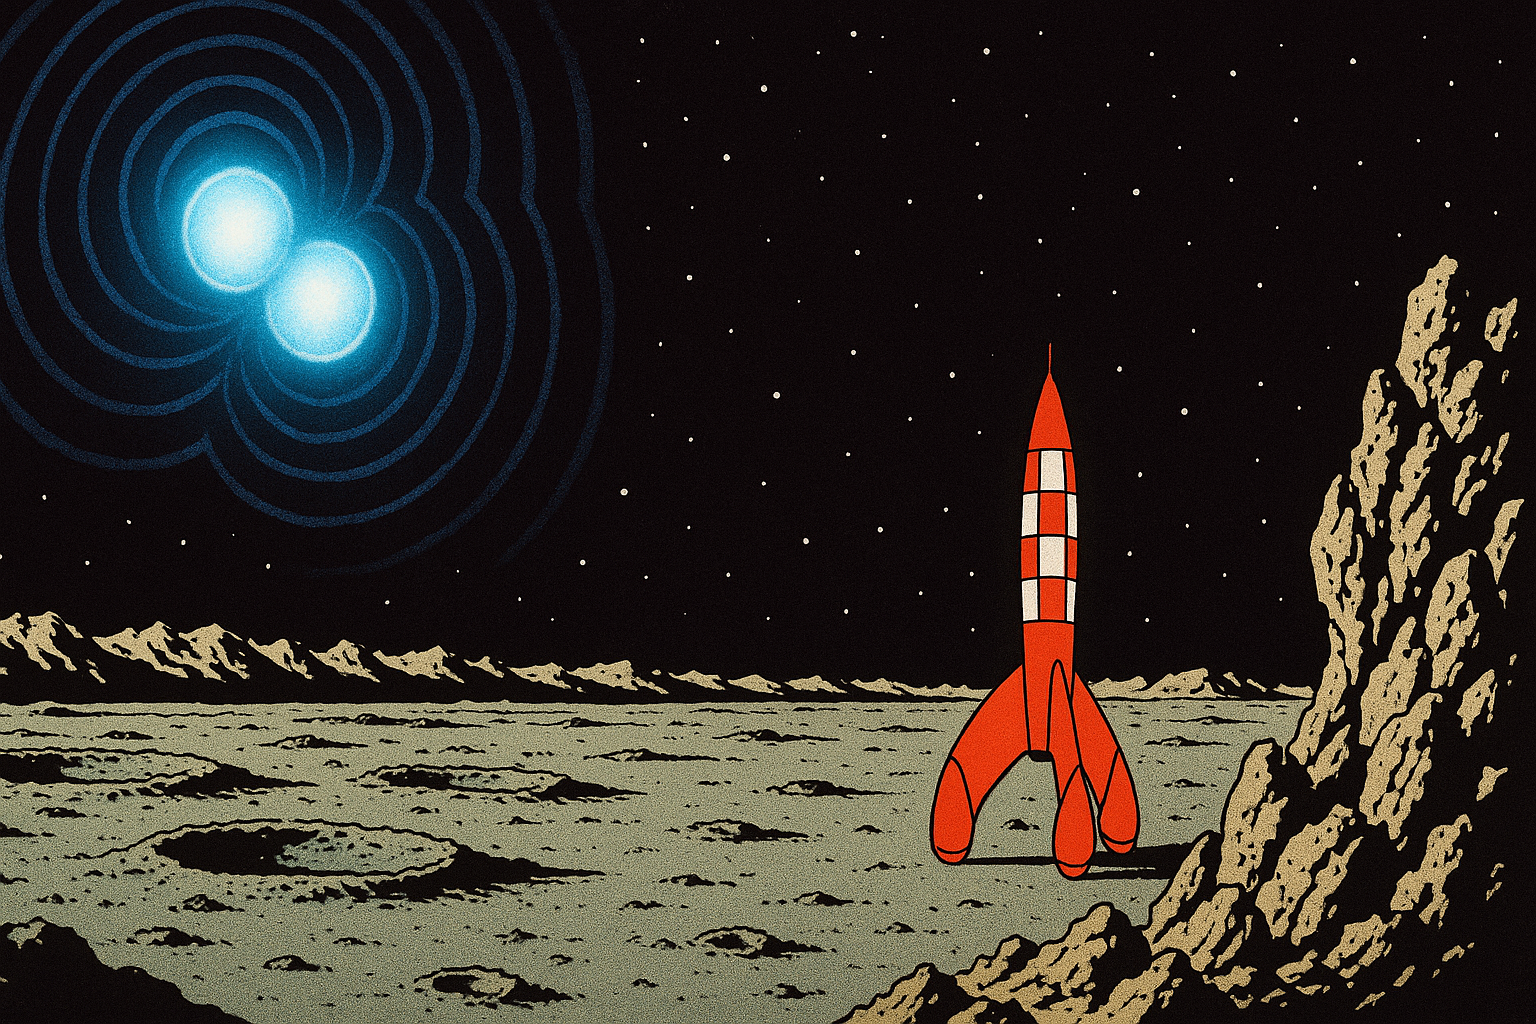
\includegraphics[width=\paperwidth,height=\paperheight]{Figures/tintin_BNS_2.png}}}

\begin{frame}[plain, noframenumbering]

  \begin{tikzpicture}[remember picture,overlay]
    \node[fill=customblue, fill opacity=0.75, text opacity=1, rounded corners=10pt, inner sep=15pt] at (current page.center) {
      \begin{minipage}{0.8\textwidth}
        \centering
        \textbf{Towards GPU-accelerated multimessenger inference of neutron star mergers and dense matter physics}\\[1.5ex]
        \normalsize Thibeau Wouters \\[0.5ex]
        \github \quad \linkedin \quad \myemail
      \end{minipage}
    };
  \end{tikzpicture}
  
  \vspace{7cm}

  \begin{columns}
  \column{0.35\textwidth}
  \begin{figure}
    \centering
    \vspace{1.5mm}
    
\includegraphics[width=0.75\linewidth]{Figures/utrecht-university.png}
  \end{figure}
  \column{0.35\textwidth}
  \begin{figure}
    \centering
    
\includegraphics[width=0.75\linewidth]{Figures/Nikhef_logo-transparent.png}
  \end{figure}
\end{columns}
  
  \end{frame}
}

% %The next statement creates the title page.
% \frame[plain]{\titlepage
% }


%---------------------------------------------------------
%This block of code is for the table of contents after the title page
% \begin{frame}[plain, noframenumbering]
% \frametitle{Table of Contents}
% \tableofcontents
% \end{frame}
%---------------------------------------------------------

\begin{frame}
\frametitle{Table of Contents}
\tableofcontents[hideallsubsections]
\end{frame}

\section{Introduction}

\subsection{Neutron stars and equation of state}

\begin{frame}{Neutron stars}

  \def\x{3mm}

  \begin{itemize}
    \item Neutron stars: supernova remnants, densest matter in the universe
    
    \item $m \sim 1.2 - 2.3 M_\odot$, $R \sim 10-13$ km
  \end{itemize}

  \pause

  \centering
  \incfig[0.90\textwidth]{NS_above_Berlin}
\end{frame}

\begin{frame}{Equation of state}

  \def\x{3mm}
  \def\y{1mm}

  Neutron stars probe the high-density part of the equation of state (EOS) of dense nuclear matter~\cite{Koehn:2024set}

  \vspace{\x}

  \begin{figure}
    \centering
    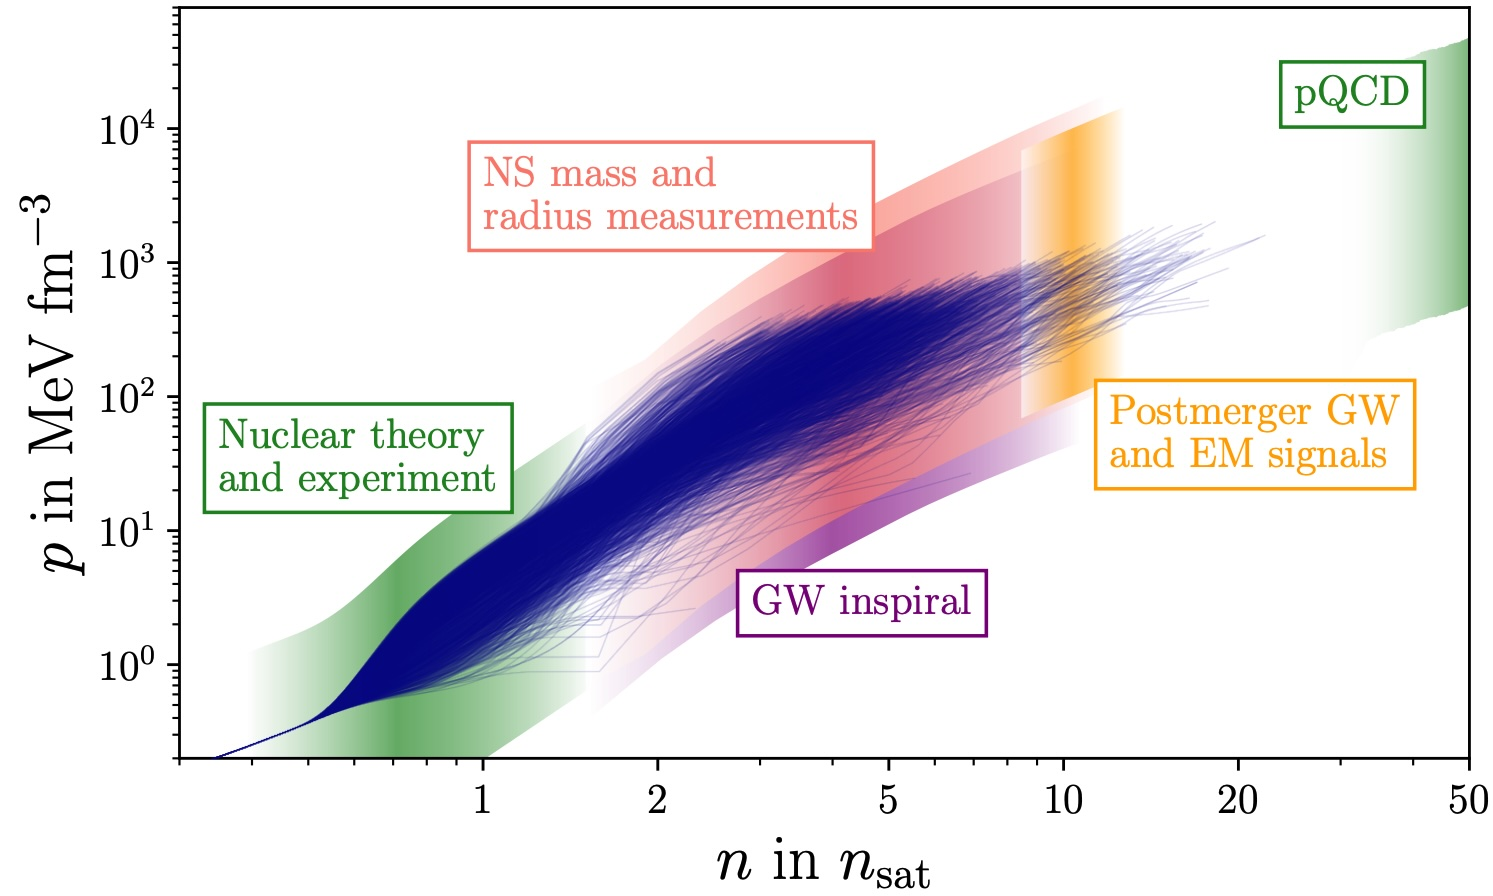
\includegraphics[width=0.85\linewidth]{Figures/Koehn_EOS.jpg}
  \end{figure}
\end{frame}


\subsection{Multimessenger astrophysics}


\begin{frame}{Multimessenger astrophysics: GW170817}

  \def\x{2mm}
  
  Neutron star mergers emit gravitational waves and electromagnetic radiation: GW170817~\cite{LIGOScientific:2017vwq, LIGOScientific:2017zic}

  \only<1>{
    \begin{figure}
      \centering
      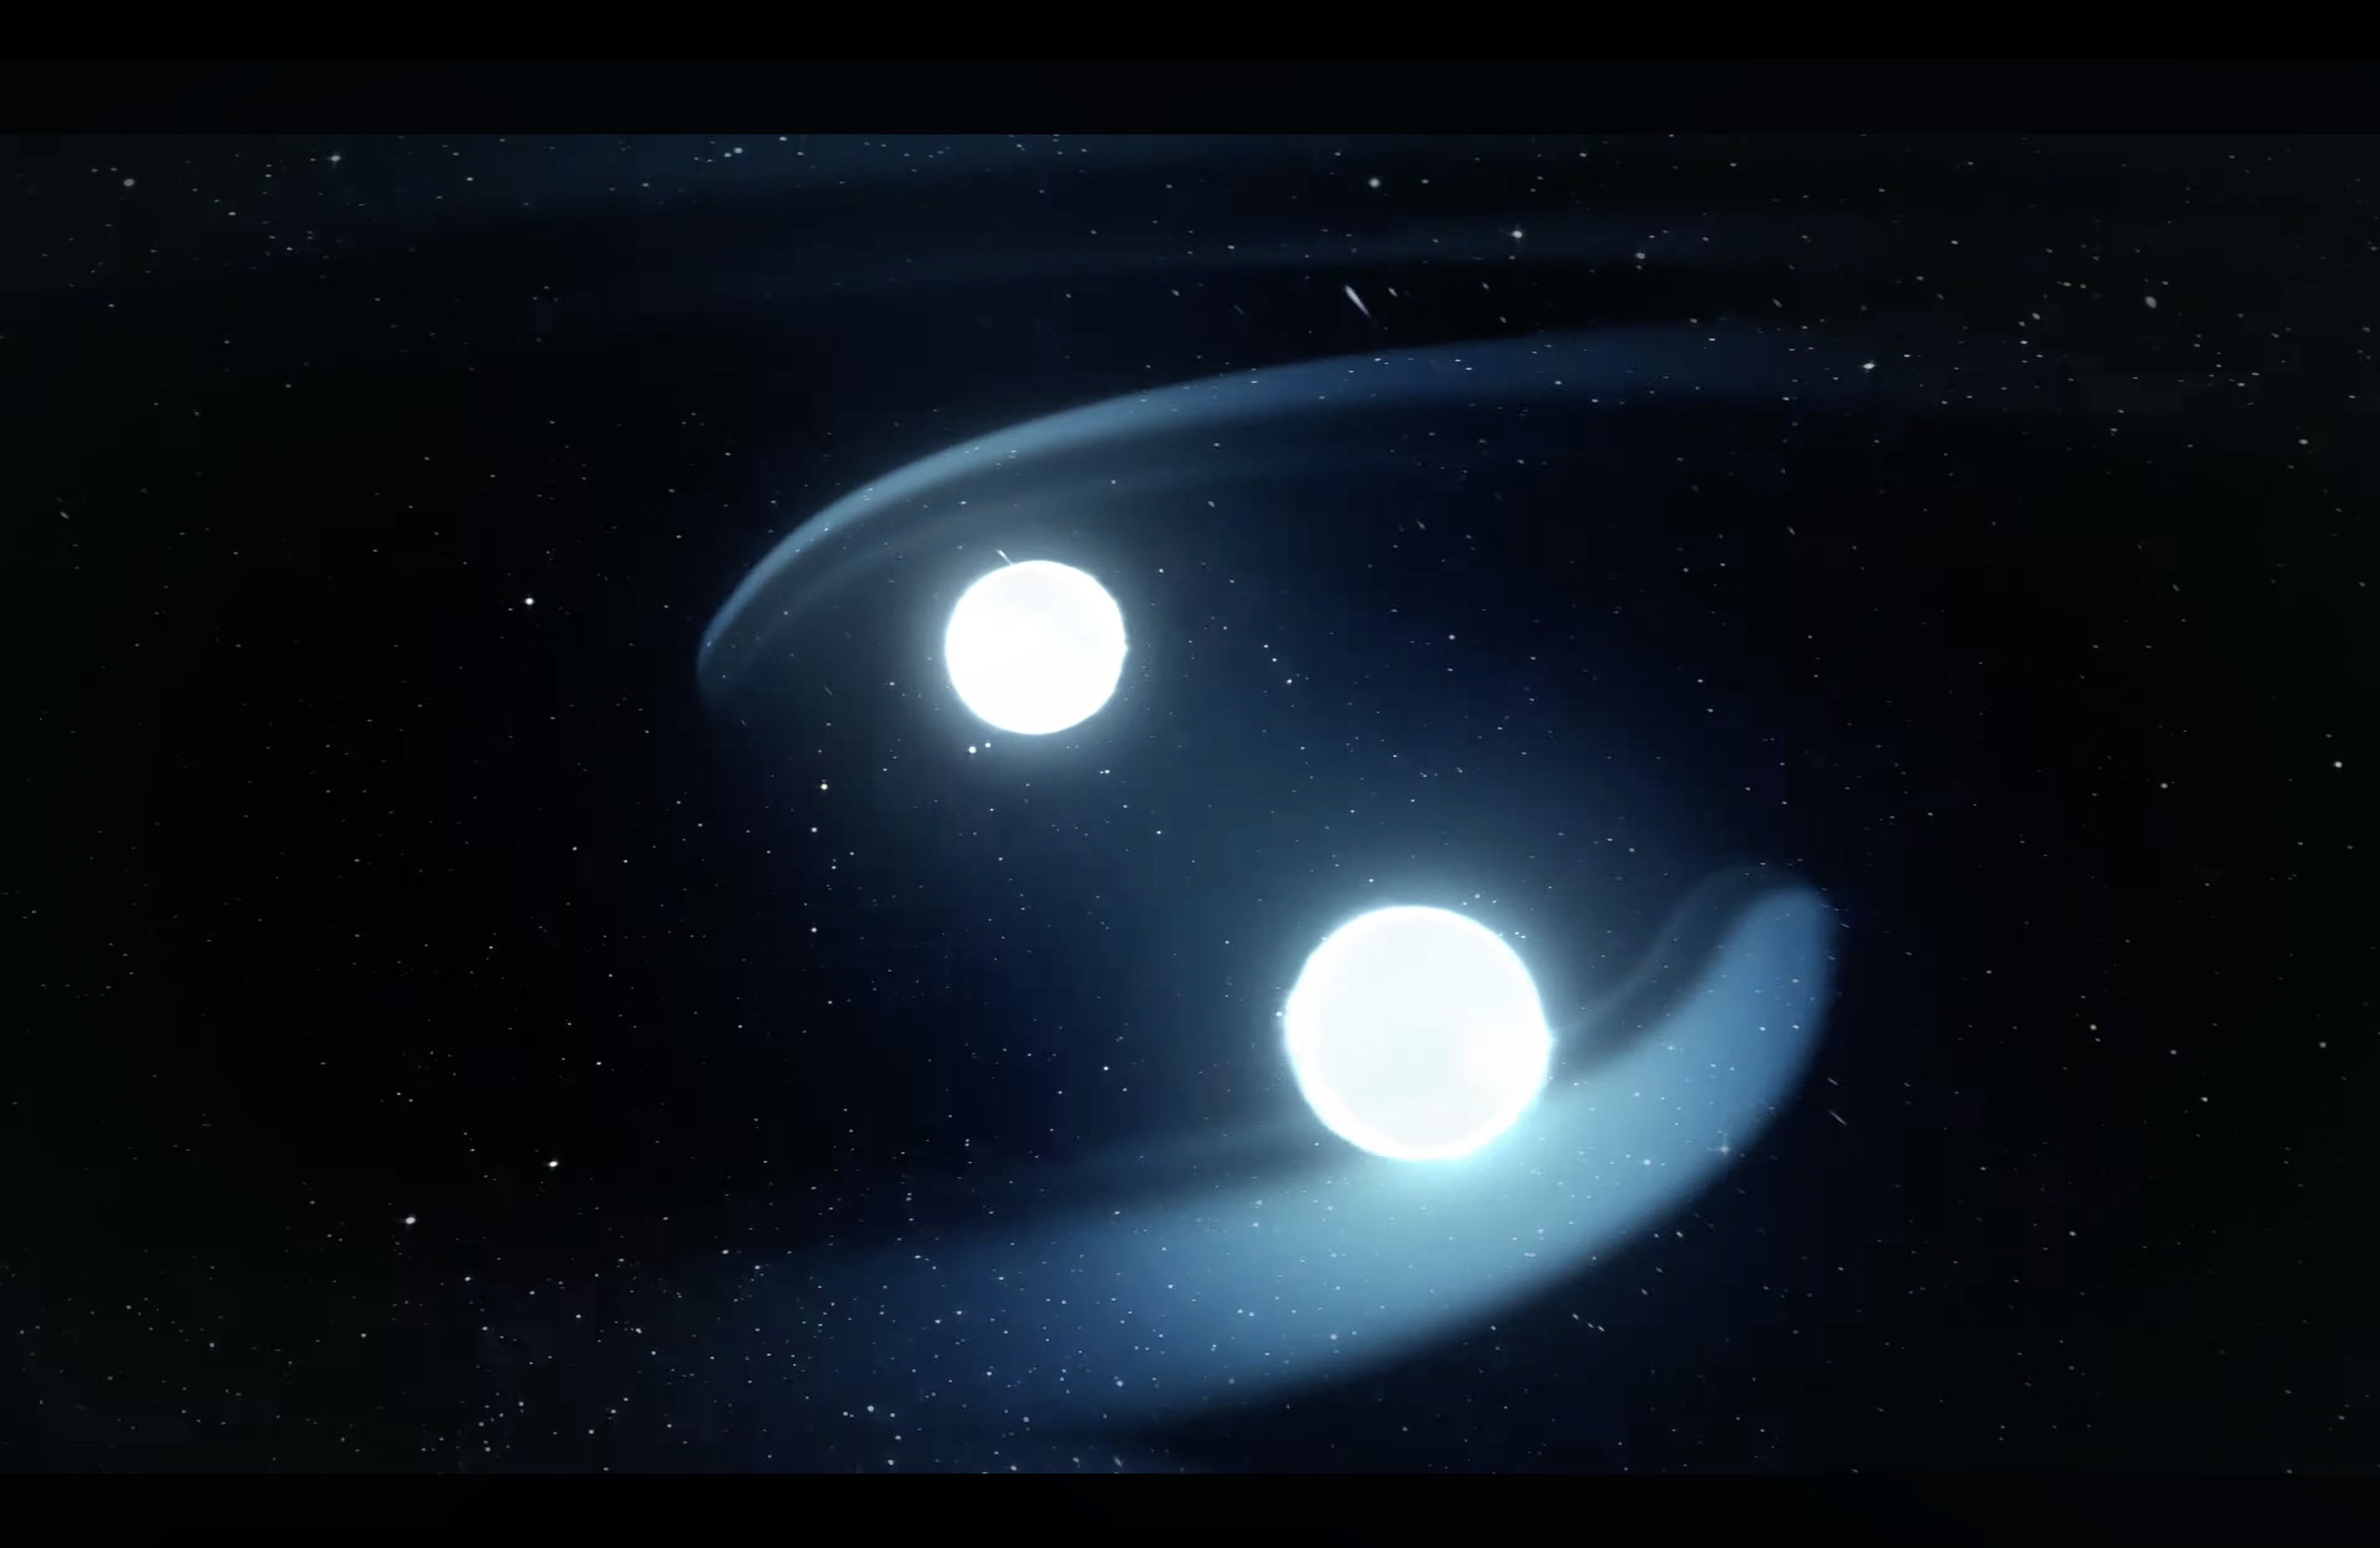
\includegraphics[width=0.95\linewidth]{Figures/GW170817_inspiral.jpg}
    \end{figure}  
  }
  
  \only<2>{
    \begin{figure}
      \centering
      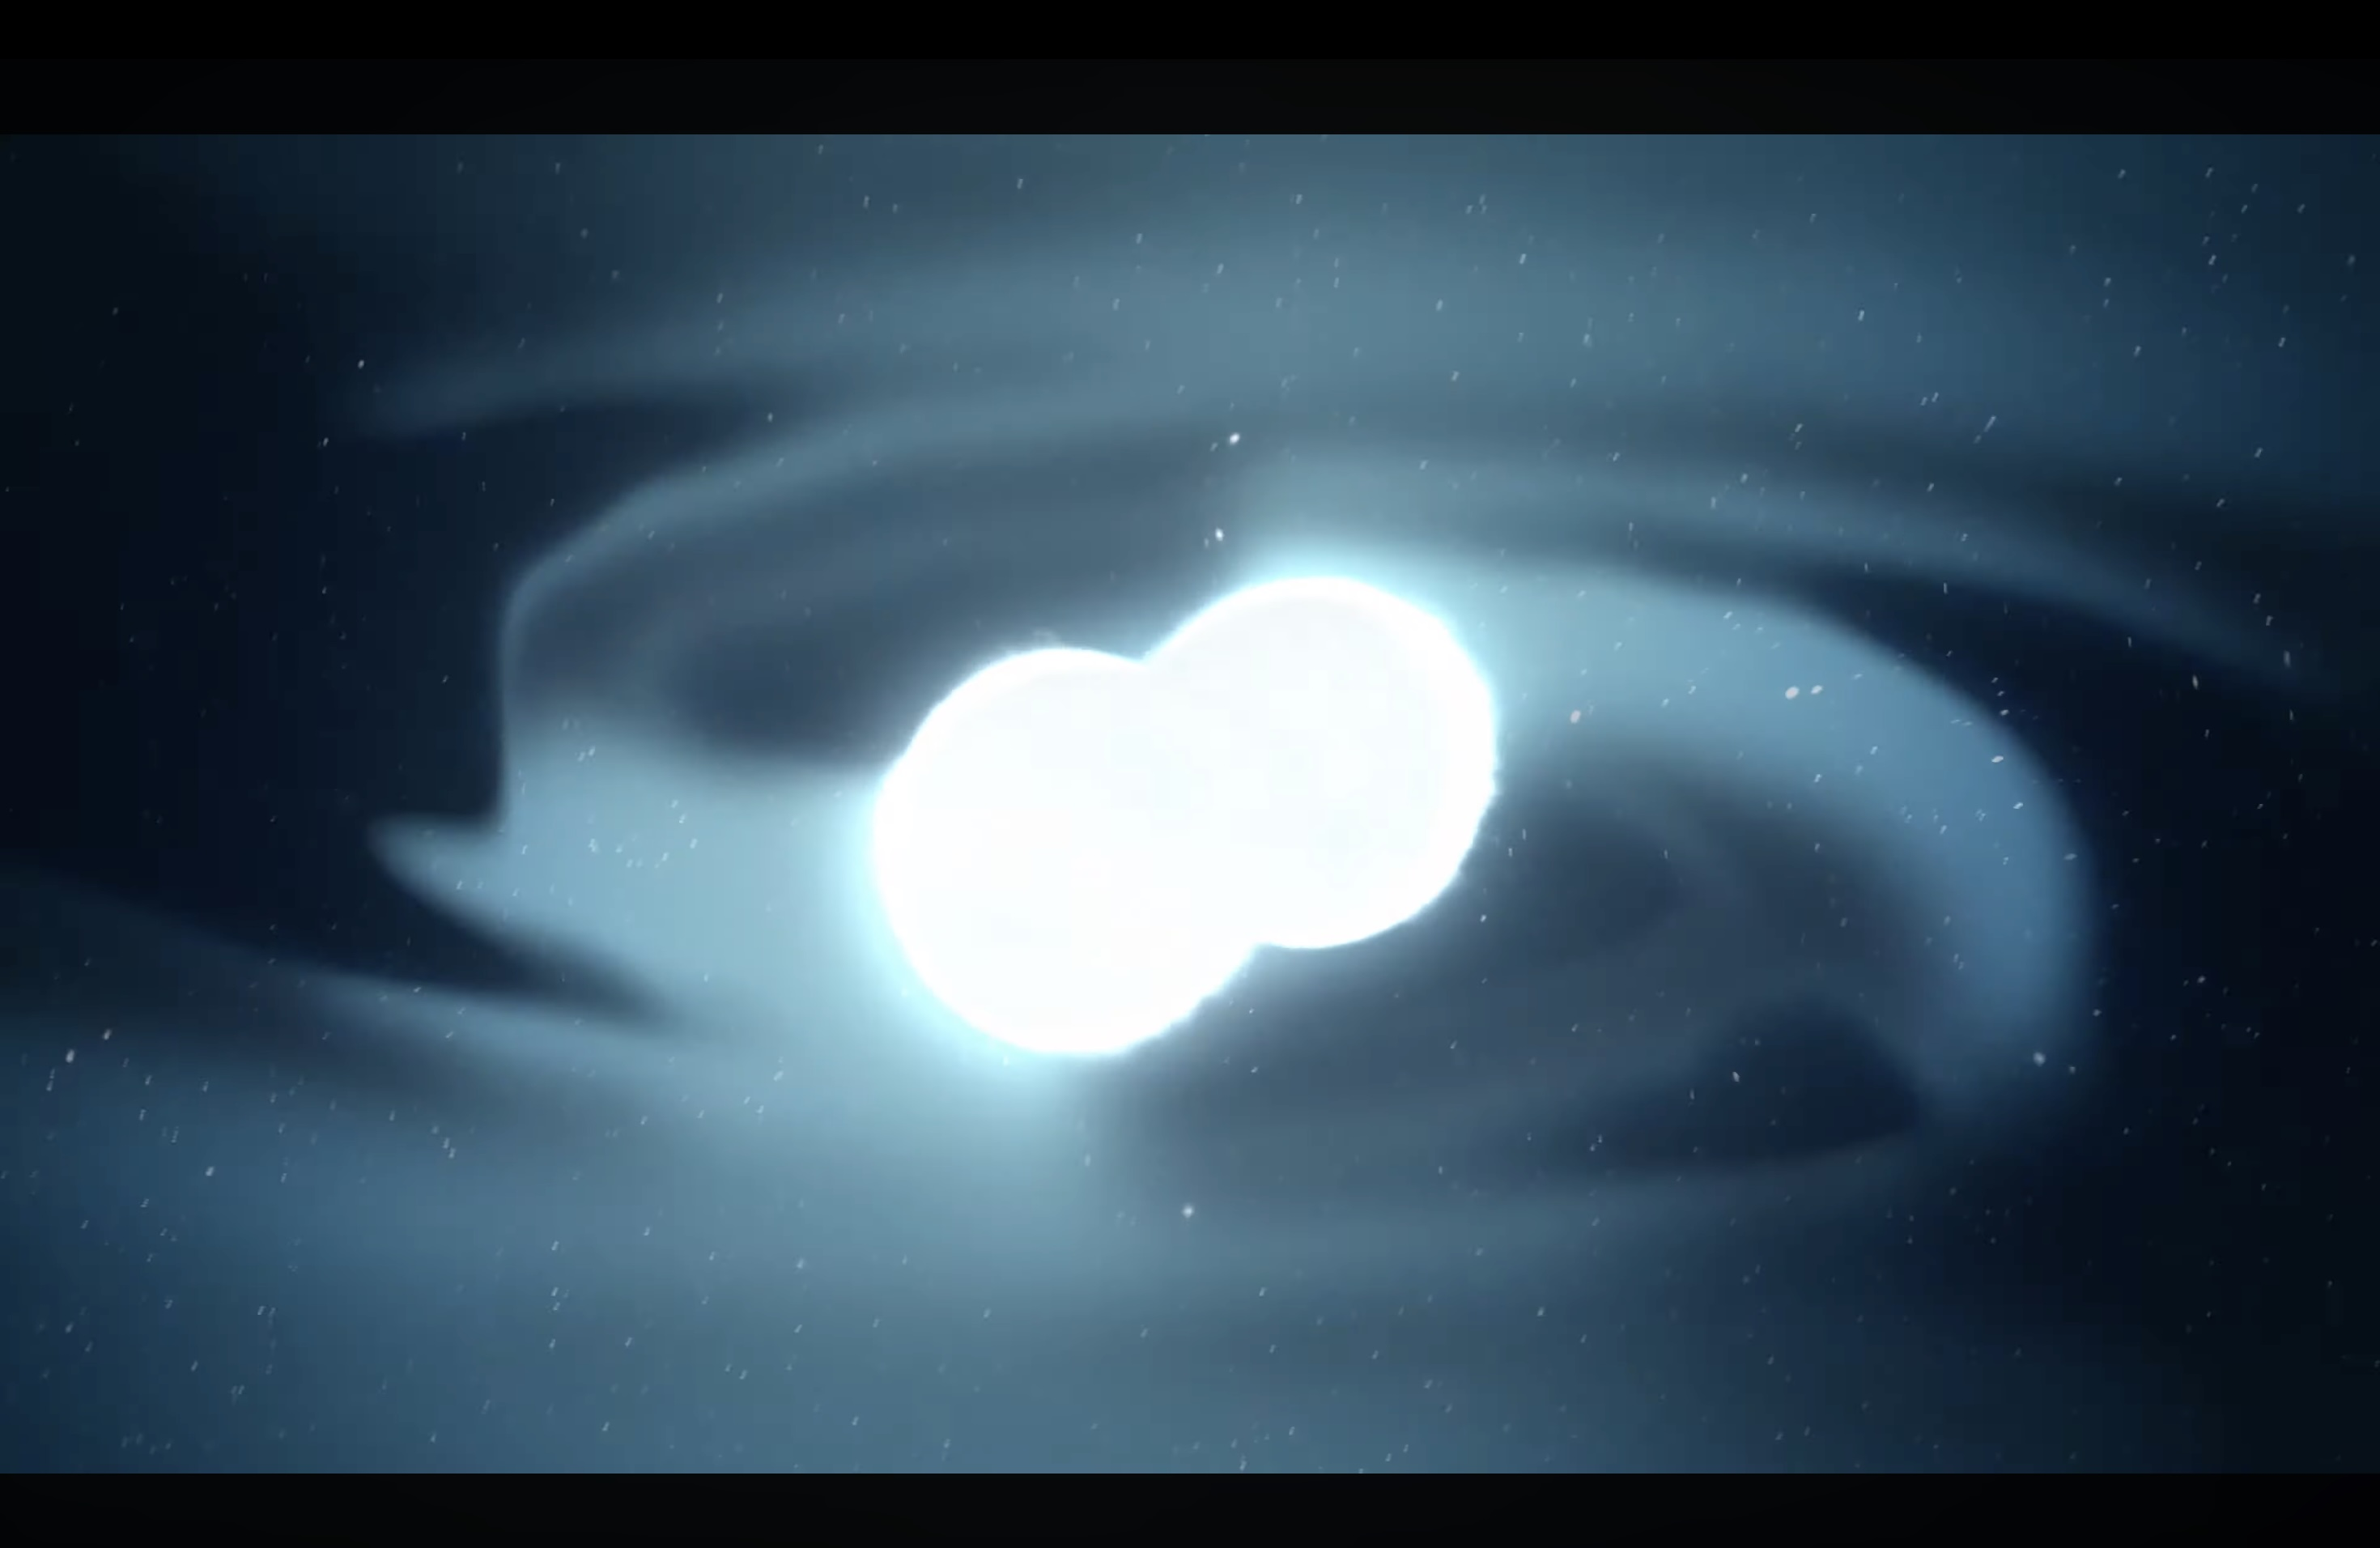
\includegraphics[width=0.95\linewidth]{Figures/GW170817_merger.jpg}
    \end{figure}  
  }
  
  \only<3>{
    \begin{figure}
      \centering
      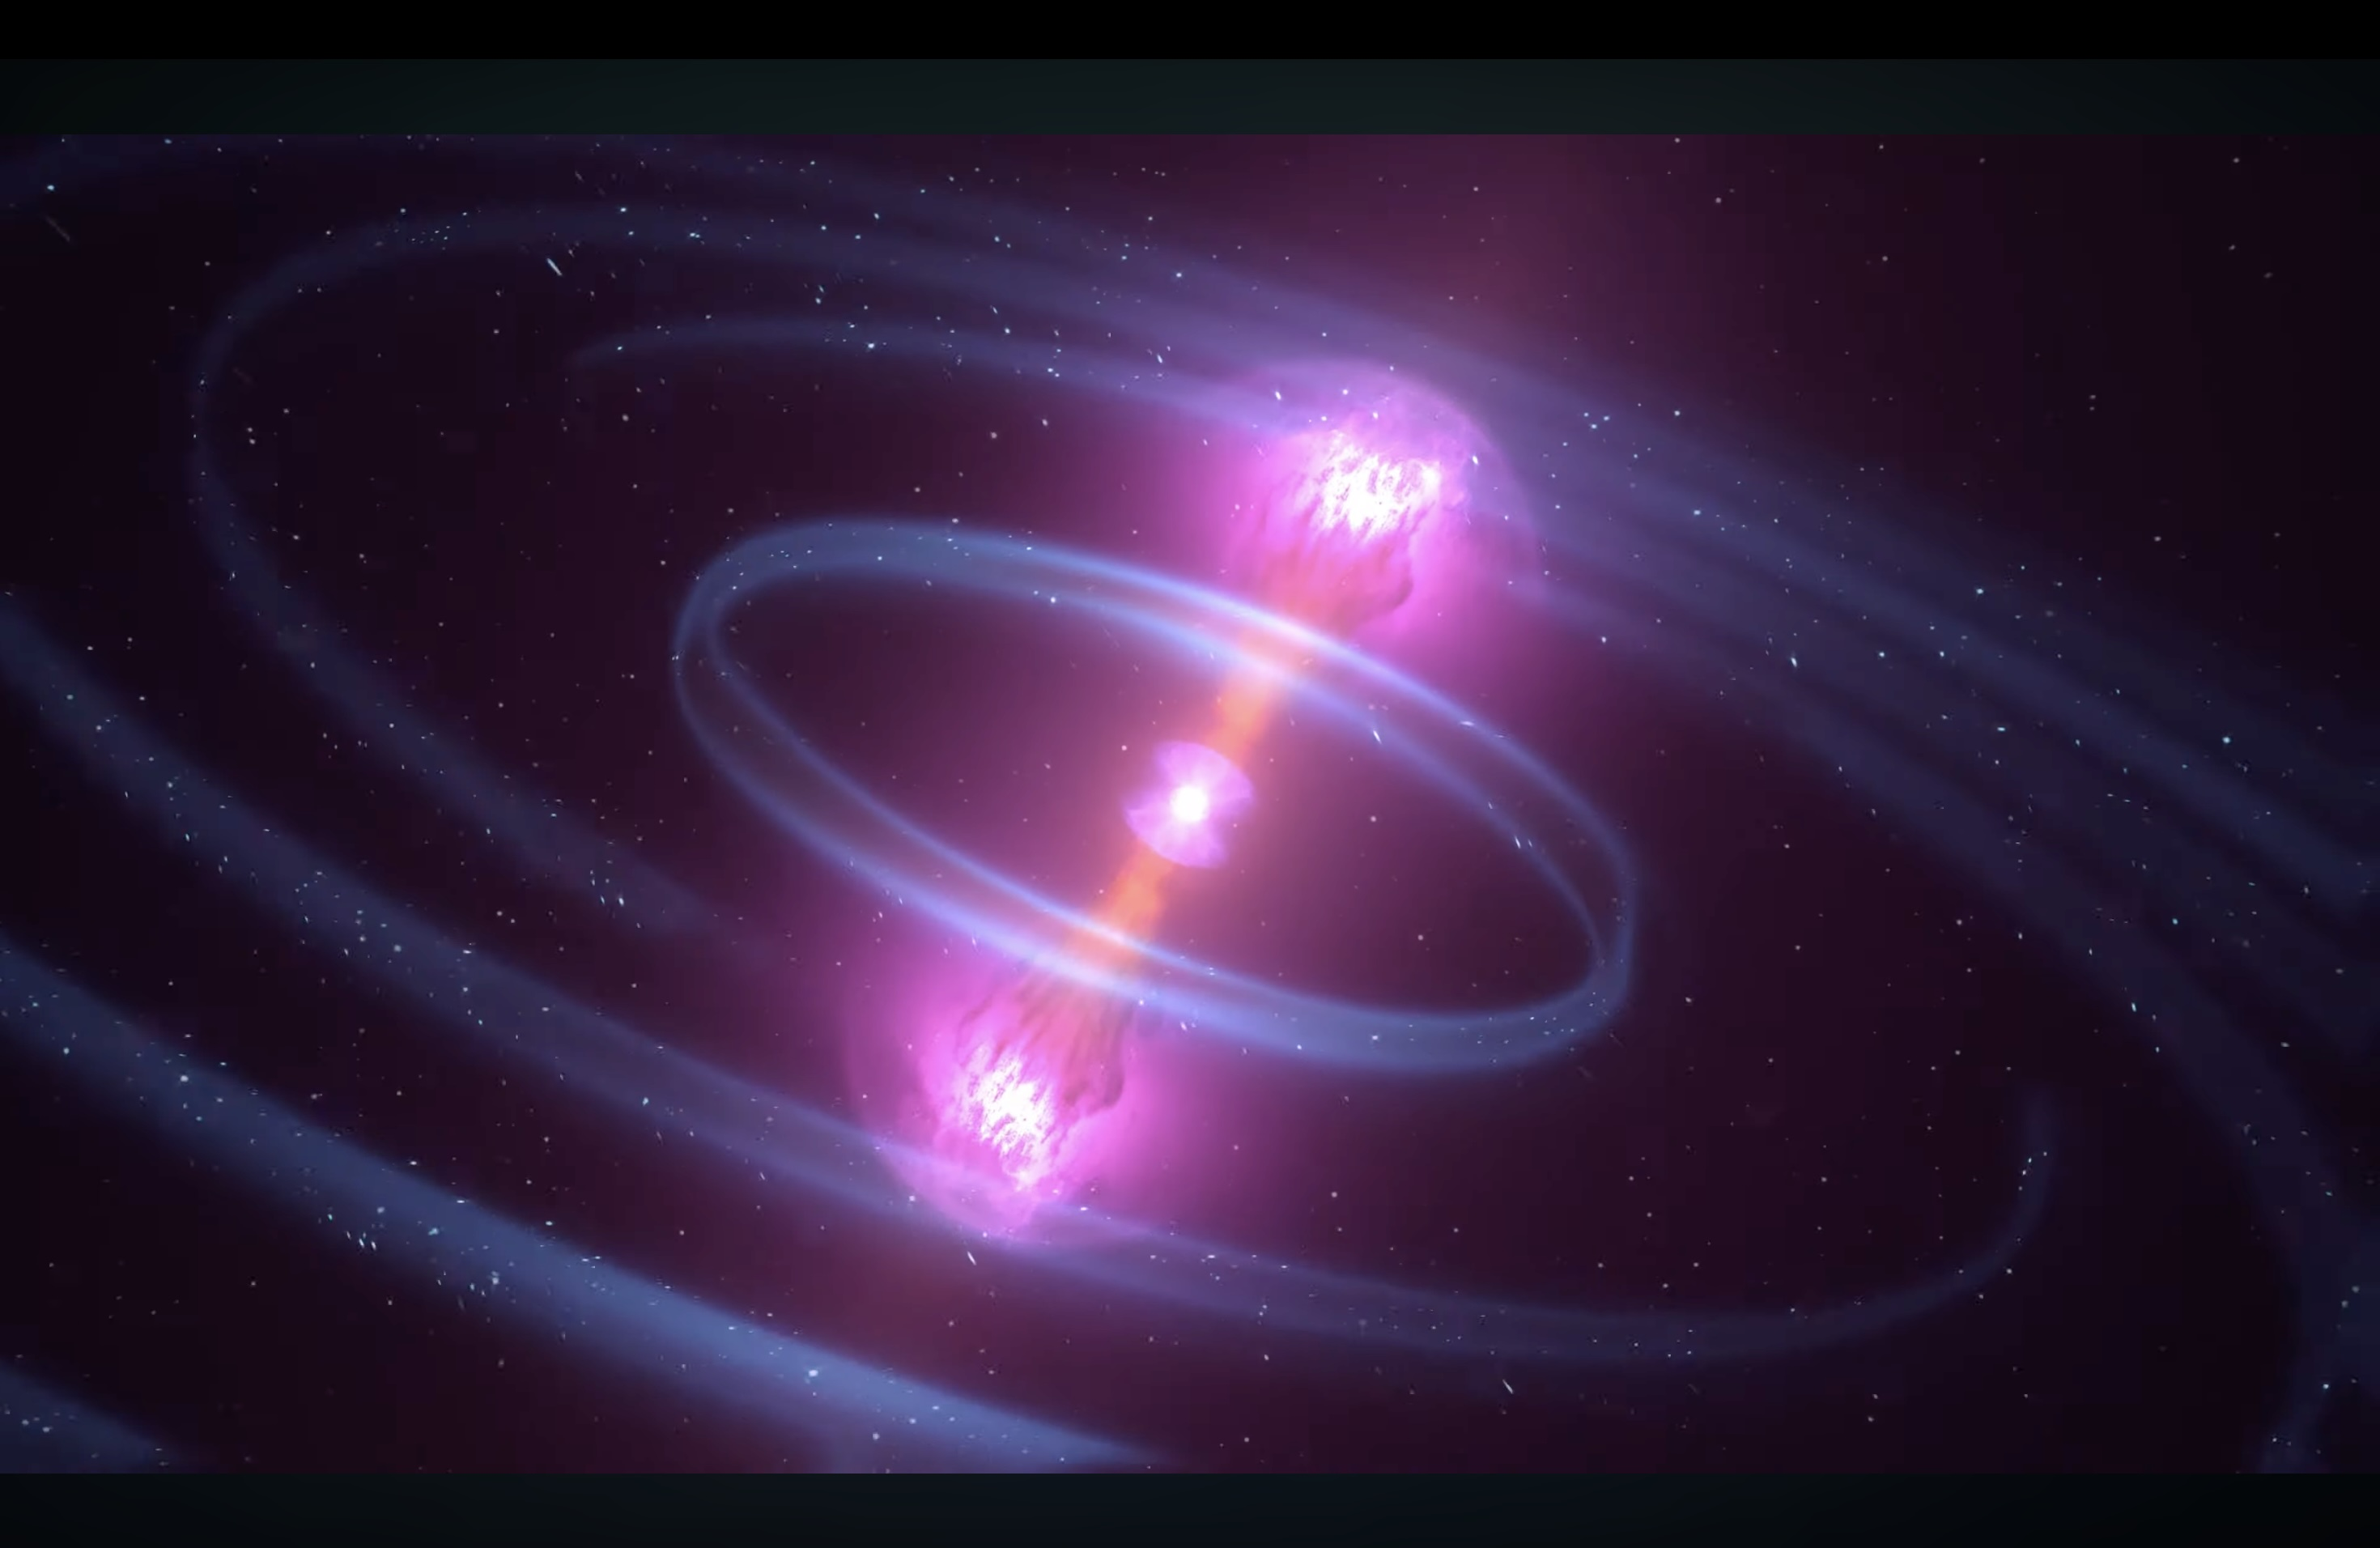
\includegraphics[width=0.95\linewidth]{Figures/GW170817_GRB.jpg}
    \end{figure}  
  }
  
  \only<4>{
    \begin{figure}
      \centering
      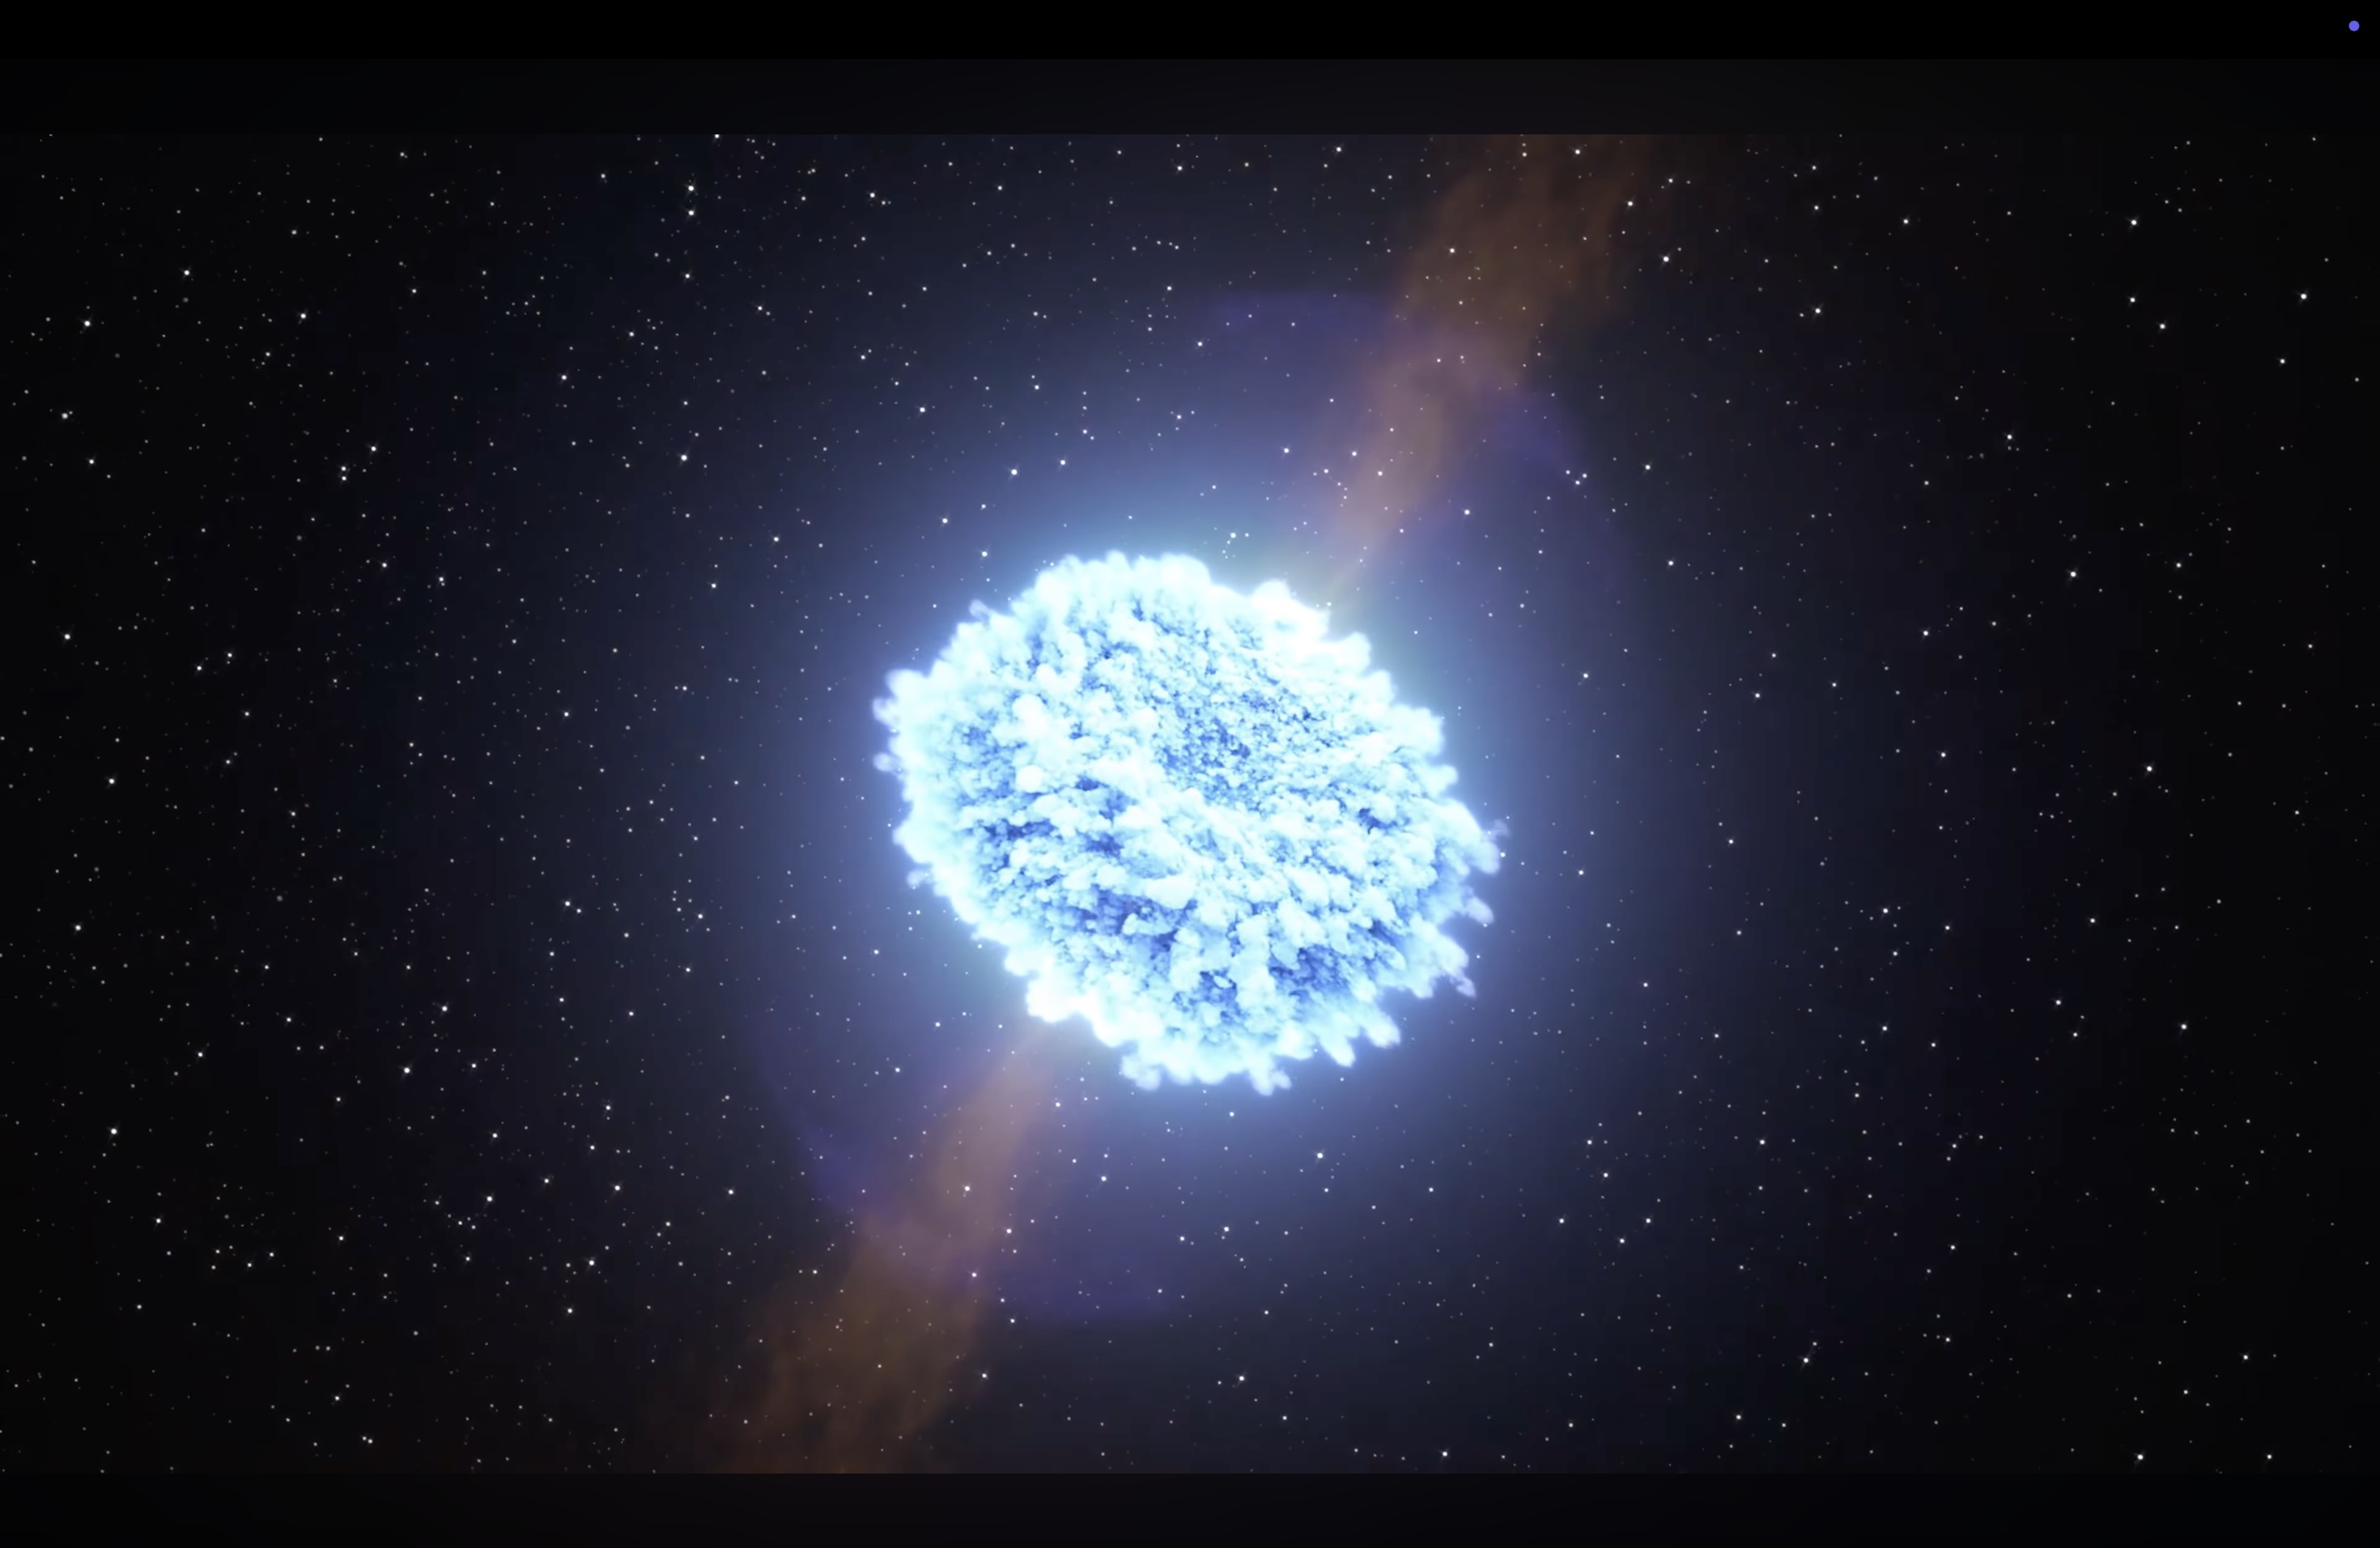
\includegraphics[width=0.95\linewidth]{Figures/GW170817_KN.jpg}
    \end{figure}  
  }
  
  \only<5>{
    \begin{figure}
      \centering
      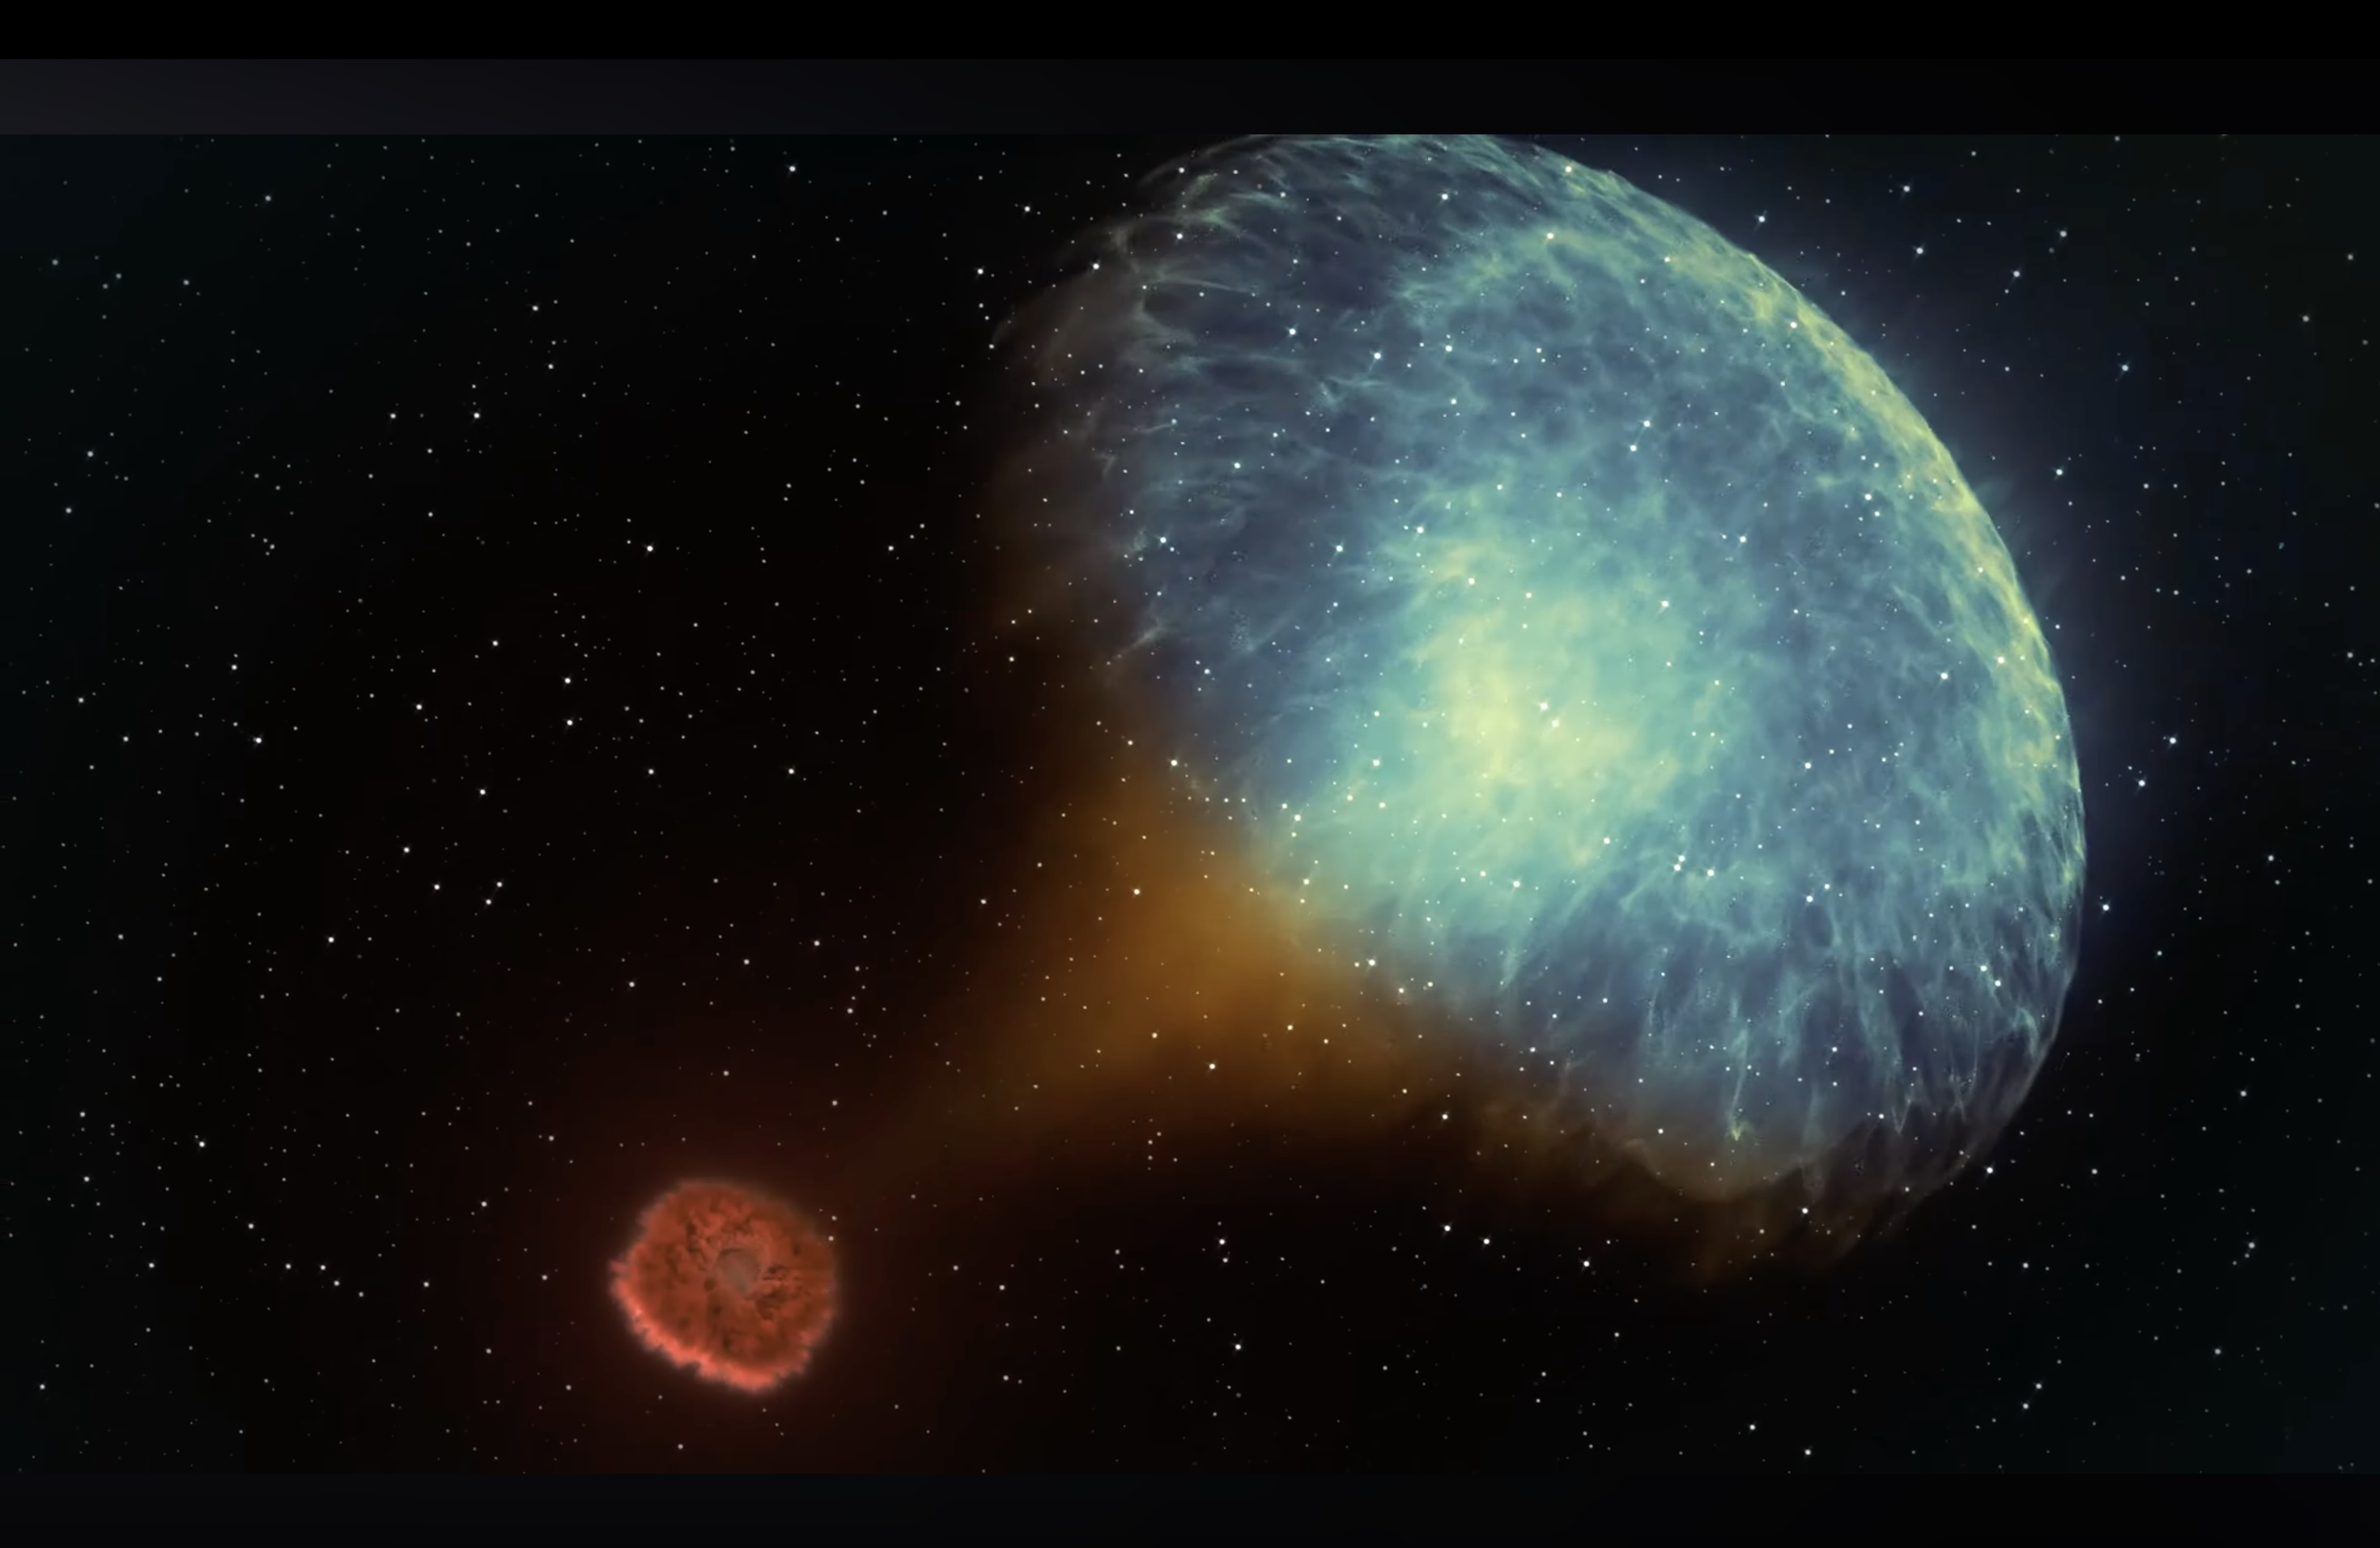
\includegraphics[width=0.95\linewidth]{Figures/GW170817_GRB_afterglow.jpg}
    \end{figure}  
  }
  
\end{frame}

\subsection{Future detectors and challenges}

\begin{frame}{Future GW detectors: Einstein Telescope}
  \def\x{3mm}
  \def\y{2mm}
  \def\z{1mm}

  \textbf{Einstein Telescope}: Third-generation ground-based GW detector~\cite{ET:2019dnz, Abac:2025saz}

  \only<1>{
    \vspace{3mm}
    \begin{figure}
      \centering
      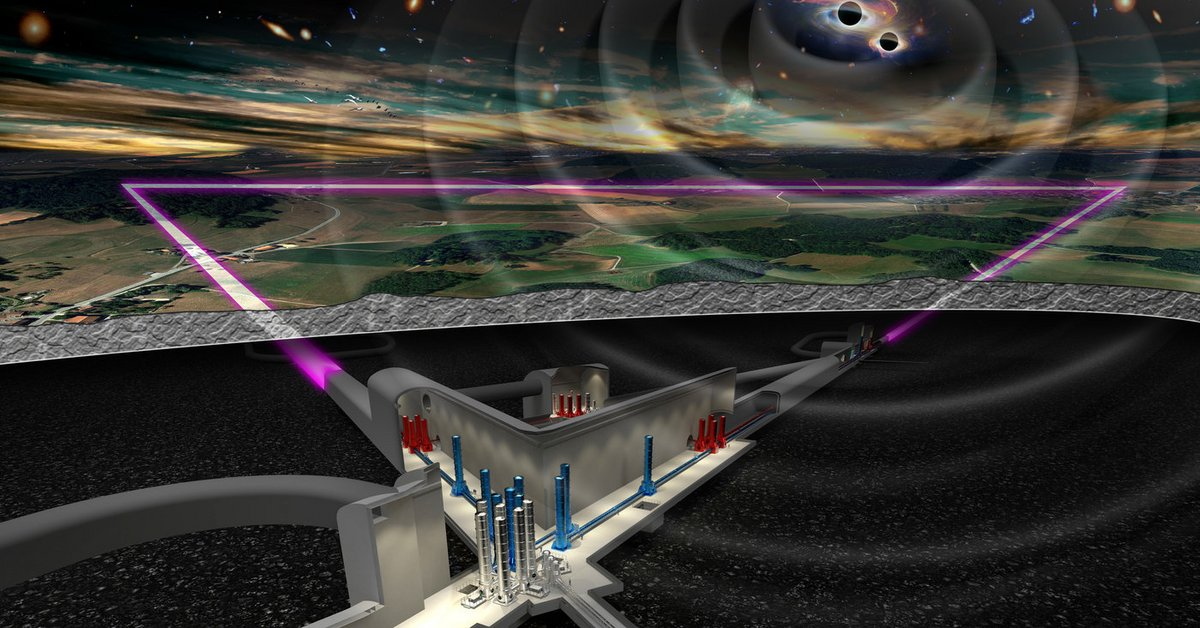
\includegraphics[width=0.95\linewidth]{Figures/ET_triangle.jpg}
    \end{figure}

    \hspace{5mm} (or 2 L-shaped detectors...)
  }

  \begin{itemize}
    \item<2-> Increased sensitivity
    
    \begin{itemize}
      \item Louder signals
      
      \vspace{\z}

      \item $10^{5} - 10^{6}$ binary black hole mergers/year (now: $\sim 200$/10 years)
      
      \vspace{\z}
      
      \item $10^{4} - 10^{5}$ binary neutron star mergers/year (now: $2$/10 years)

      \vspace{\z}
      
      \item $10^{2} - 10^{3}$ multimessenger events/year (now: $1$/10 years)
    \end{itemize}

    \vspace{\y}

    \item<3-> Observe from $5$ Hz (now: $20$ Hz)
    \begin{itemize}
      
      \item Longer signals
      \begin{itemize}
        \item Binary neutron star: $2$ hours (vs 2 minutes now)
      \end{itemize}
      \item Signals will overlap: joint analysis needed
    \end{itemize}
  \end{itemize}

  \vspace{4mm}

  \onslide<4->{
  \begin{tcolorbox}[colback=red!10!white, colframe=red!80!black, coltext=black]
  Current software cannot handle the ET data analysis problem~\cite{Hu:2024mvn}
  \end{tcolorbox}
  }
\end{frame}


\begin{frame}{My research focus: why -- how -- what}
  \def\y{0.5mm}

  \vspace{-6mm}

  \begin{tcolorbox}[colback=jaxbluedarkcolor!15!white, colframe=jaxbluedarkcolor!80!black, coltext=black]
  \textbf{Why?}

  To make inference of multimessenger astrophysics scalable

  \begin{itemize}
    \vspace{\y}
    \item Prepare for future detectors

    \vspace{\y}

    \item Understand systematic effects through simulated data
  \end{itemize}
  \end{tcolorbox}

  \pause

  \begin{tcolorbox}[colback=jaxgreendarkcolor!15!white, colframe=jaxgreendarkcolor!80!black, coltext=black]
  \textbf{How?}

  Without compromises to flexibility and accuracy

  \begin{itemize}
    \vspace{\y}
    \item Accelerate with GPU hardware, differentiable programming

    \vspace{\y}

    \item Use machine learning to assist inference, not replace it
  \end{itemize}
  \end{tcolorbox}

  \pause

  \begin{tcolorbox}[colback=jaxthreecolor!15!white, colframe=jaxthreecolor!80!black, coltext=black]
  \textbf{What?}

  GPU-accelerated Bayesian joint inference framework of neutron star mergers and dense matter physics
  \end{tcolorbox}
\end{frame}


\section{Methods}

\subsection{Bayesian inference and sampling}

\begin{frame}{Parameter estimation: Bayesian inference}

  \def\x{5mm}

  How do we ``measure'' source parameters $\theta$ for data $d$? 

  \vspace{\x}
  \pause
  
  Bayesian inference:
  \begin{equation*}
    {\rm{posterior}} = p(\theta|d, \mathcal{M}) = \frac{p(d|\theta, \mathcal{M}) p(\theta | \mathcal{M})}{p(d | \mathcal{M})} = \frac{\rm{likelihood} \times \rm{prior}}{\rm{evidence}}
  \end{equation*}

  \vspace{\x}
  \pause

  Ingredients:
  \begin{itemize}
    \item Posterior: intractable, needs stochastic samplers
    
    \item Prior: specified by users, encode beliefs
    
    \item Likelihood: \red{computational bottleneck}

    \item Evidence: model selection
  \end{itemize}
\end{frame}


\begin{frame}{Parameter estimation: Markov chain Monte Carlo}

  \def\x{3mm}

  How do we sample the posterior? \red{Markov chain Monte Carlo}

  \begin{itemize}
    \item $N$ chains $\boldtheta_i$ explore posterior in parallel
    
    \item Evolve chains to new position: proposal 
    
    \item Compute likelihood $\rightarrow$ \mcmcgreen{accept}/\mcmcred{reject}
  \end{itemize}
  
  \vspace{\x}

  Alternatives: nested sampling, sequential Monte Carlo

  \vspace{\x}

  \centering
  \incfig[0.9\textwidth]{sampling}

  \vspace{\x}

  
\end{frame}

\begin{frame}<1-4>[label=compaspects]{Computational aspects}

  \def\x{3mm}
  \def\y{1mm}

  \begin{equation*}
    {\rm{Total \ runtime}} \approx \red{N_{{\rm{likelihood}}}} \times \blue{\tau_{{\rm{likelihood}}}}
  \end{equation*}

  \pause

  \begin{itemize}
    \item $\red{N_{{\rm{likelihood}}}}$: total number of likelihood evaluations
    \begin{itemize}
      \item Dimensionality of $\boldtheta$
      
      \vspace{\y}
      
      \item Signal-to-noise ratio
      
      \vspace{\y}
      
      \item Multimodality/shape posterior
      
      \vspace{\y}

      \item \alt<4->{\textbf{Efficiency of sampler (proposals)}}{Efficiency of sampler (proposals)}

    \end{itemize}

    \vspace{\x}
    \pause

    \item $\blue{\tau_{{\rm{likelihood}}}}$: speed of a single likelihood evaluation
    \begin{itemize}
      \item Complexity model/likelihood function

      \vspace{\y}

      \item \alt<4->{\textbf{Parallelization of likelihood evaluations}}{Parallelization of likelihood evaluations}


      \vspace{\y}
      
      \item \alt<4->{\textbf{Hardware}}{Hardware}
    \end{itemize}
  \end{itemize}

  \pause
  \vspace{6mm}

  \textbf{How can we optimize this?}
\end{frame}

\subsection{\textsc{jax}}


\begin{frame}{\textsc{jax}}

  \def\x{5mm}
  \def\y{1mm}

  \begin{columns}
    \begin{column}{0.84\linewidth}
      \textbf{\textsc{jax}}~\ghlink{jax-ml/jax}
      ``is a Python library for accelerator-oriented array computation and program transformation, designed for \red{high-performance} numerical computing and large-scale machine learning.''~\cite{jax2018github}
    \end{column}
    \begin{column}{0.15\linewidth}
      \begin{figure}
        \centering
        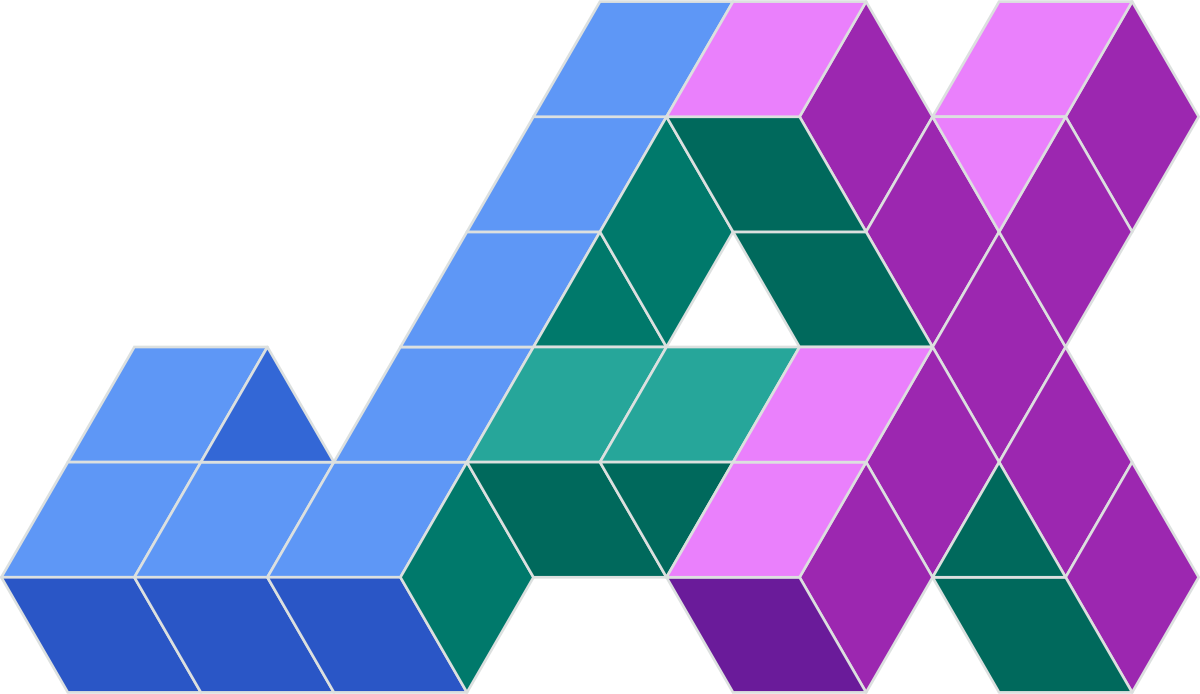
\includegraphics[width=0.95\linewidth]{Figures/jax.png}
      \end{figure}
    \end{column}
  \end{columns}

  \vspace{\x}
  \pause

  In particular:
  \begin{itemize}
    \vspace{\y}
    \item Python: integrate into existing workflows

    \vspace{\y}

    \item Focus on arrays: widespread applications
    
    \vspace{\y}

    \item Numpy-like API: (\texttt{numpy} $\rightarrow$ \texttt{jax.numpy})
  \end{itemize}

  \pause
  \vspace{4mm}

  \red{Gamechangers}:
  \begin{itemize}
    \item GPU accelerators
    
    \vspace{\y}

    \item Composable function transformations: \jaxjit, \jaxgrad, \jaxvmap~\& \jaxpmap
  \end{itemize}
\end{frame}

\begin{frame}{\textsc{jax} -- Function transformations}

  \def\x{8mm}
  \def\y{2mm}

  \begin{itemize}
    \item \jaxjit: Just-in-time compilation
    
    \vspace{\y}
    
    \item<2-> \jaxgrad: Automatic differentiation:
    \begin{itemize}
      \item Chain rule on computational graph
      
      \item Exact gradients (up to machine precision), fast
    \end{itemize}
    
    \vspace{\y}
    
    \item<3-> \jaxvmap, \jaxpmap: Vectorization, batch processing, parallelization
    
    \vspace{\x}

    \item<4-> These are composable, e.g.:
    \begin{itemize}
      \item Higher-order derivatives: \texttt{\jaxgrad(\jaxgrad(f))}
      
      \item Evolve $N$ chains in parallel along gradient of the likelihood
      \begin{equation*}
        \boldtheta \leftarrow \boldtheta + \alpha * \jaxvmap\left(  \jaxjit(\jaxgrad(\texttt{logL}(\boldtheta))) \right)
      \end{equation*}
    \end{itemize}
  \end{itemize}
\end{frame}

\againframe<5->{compaspects}

\subsection{Normalizing flows}

\begin{frame}{Normalizing flows}
  \def\x{2mm}

  \textbf{Q}: Given samples $\{\red{x}\} \sim \red{p(x)}$, how can we get $\red{p(x)}$?
  \begin{itemize}
    \item Evaluate density at any point

    \item Generate new samples
  \end{itemize}

  \vspace{2mm}
  \pause

  \textbf{A}: Normalizing flows: generative machine learning model, bijection between \blue{latent} space (Gaussian) and \red{data} space

  \vspace{-2mm}

  \centering
  \incfig[0.85\textwidth]{NF}
\end{frame}

\subsection{\textsc{flowMC}}

\begin{frame}{\textsc{flowMC}}
  \def\y{1mm}

  \textsc{flowMC}~\ghlink{kazewong/flowMC}~\cite{Gabrie:2021tlu, Wong:2022xvh}: normalizing flow-enhanced MCMC

  \begin{enumerate}
    \vspace{\y}

    \item Run gradient-based sampler (local sampler)
    
    \vspace{\y}

    \item Train normalizing flow on MCMC chains
    
    \vspace{\y}

    \item Propose samples from the normalizing flow (global sampler)

    \vspace{\y}

    \item Repeat
  \end{enumerate}

  \vspace{10mm}

  \centering
  \incfig[0.95\textwidth]{flowMCOverview2}
\end{frame}

\section{Applications}

\begin{frame}{Overview}
  \showoverview{1}
\end{frame}

\begin{frame}{Gravitational waves: \textsc{ripple}}
  \def\x{3mm}
  \def\y{5mm}
  \def\z{2mm}

  \vspace{-3mm}
  
  \begin{columns}
    \begin{column}[t]{0.62\linewidth}
      \begin{itemize}
        \item \red{Waveforms} on GPU: $\mathcal{O}(10^3)$ faster

        \vspace{\z}
        
        \item \textsc{ripple}~\ghlink{tedwards2412/ripple/}~\cite{Edwards:2023sak}: from \textsc{lalsuite} to \textsc{jax}
      \end{itemize}
    \end{column}

    \begin{column}[t]{0.36\linewidth}
      \begin{figure}
        \centering
        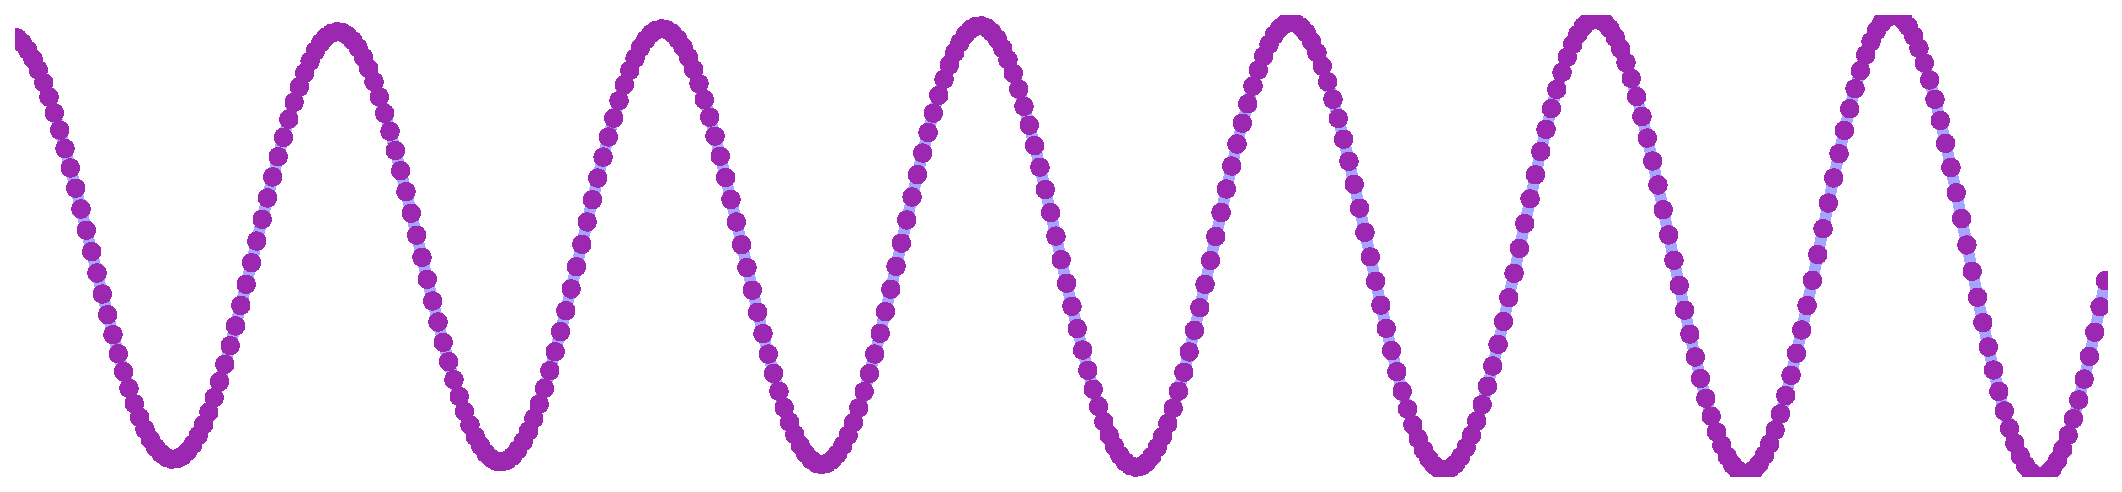
\includegraphics[width=0.99\linewidth]{Figures/strain_zoomed.pdf}
      \end{figure}
    \end{column}
  \end{columns}

  \pause
  \vspace{\x}

  \begin{itemize}
    \item Waveforms available in \textsc{ripple}:
    
    \vspace{\z}

      \begin{itemize}
        \item Binary black holes:
      \begin{itemize}
        \item \texttt{IMRPhenomXAS}
        \item \texttt{IMRPhenomD}
        \item \texttt{IMRPhenomPv2}
      \end{itemize}
      \end{itemize}

      \vspace{\z}
      
      \begin{itemize}
        \item Binary neutron stars:
      \begin{itemize}
        \item \texttt{TaylorF2}
        \item \texttt{IMRPhenomD\_NRTidalv2}
        \item \texttt{IMRPhenomPv\_NRTidalv2} (by Nihar Gupte)
      \end{itemize}
      \end{itemize}

      \vspace{\z}

      \item Also see \textsc{gwfast}~\ghlink{CosmoStatGW/gwfast}~\cite{Iacovelli:2022mbg} and \textsc{sfts}~\ghlink{rodrigo-tenorio/sfts}~\cite{Tenorio:2025gci}
  \end{itemize}

\end{frame}


\begin{frame}{Gravitational waves: \textsc{Jim}}

  \def\x{3mm}
  \def\y{5mm}
  \def\z{1mm}

  \red{Parameter estimation}: \textsc{Jim}~\ghlink{kazewong/jim}~\cite{Wong:2023lgb,Wouters:2024oxj}: \textsc{ripple} + \textsc{flowMC}

  \begin{itemize}
    
    \item Verified for binary neutron stars in current generation detectors~\cite{Wouters:2024oxj}

    \vspace{\z}

    \item Matches \textsc{bilby}, passes $pp$-test

    \vspace{\z}

    \item<2-> Runtime: from hours to minutes

    \vspace{\z}

    \item<3-> Up to $5 - 10 \times$ more effective samples (normalizing flow)

    \vspace{\z}
    
    \item<4-> More cost-effective/energy-efficient
  \end{itemize}

  \only<2>{
    \begin{figure}
      \centering
      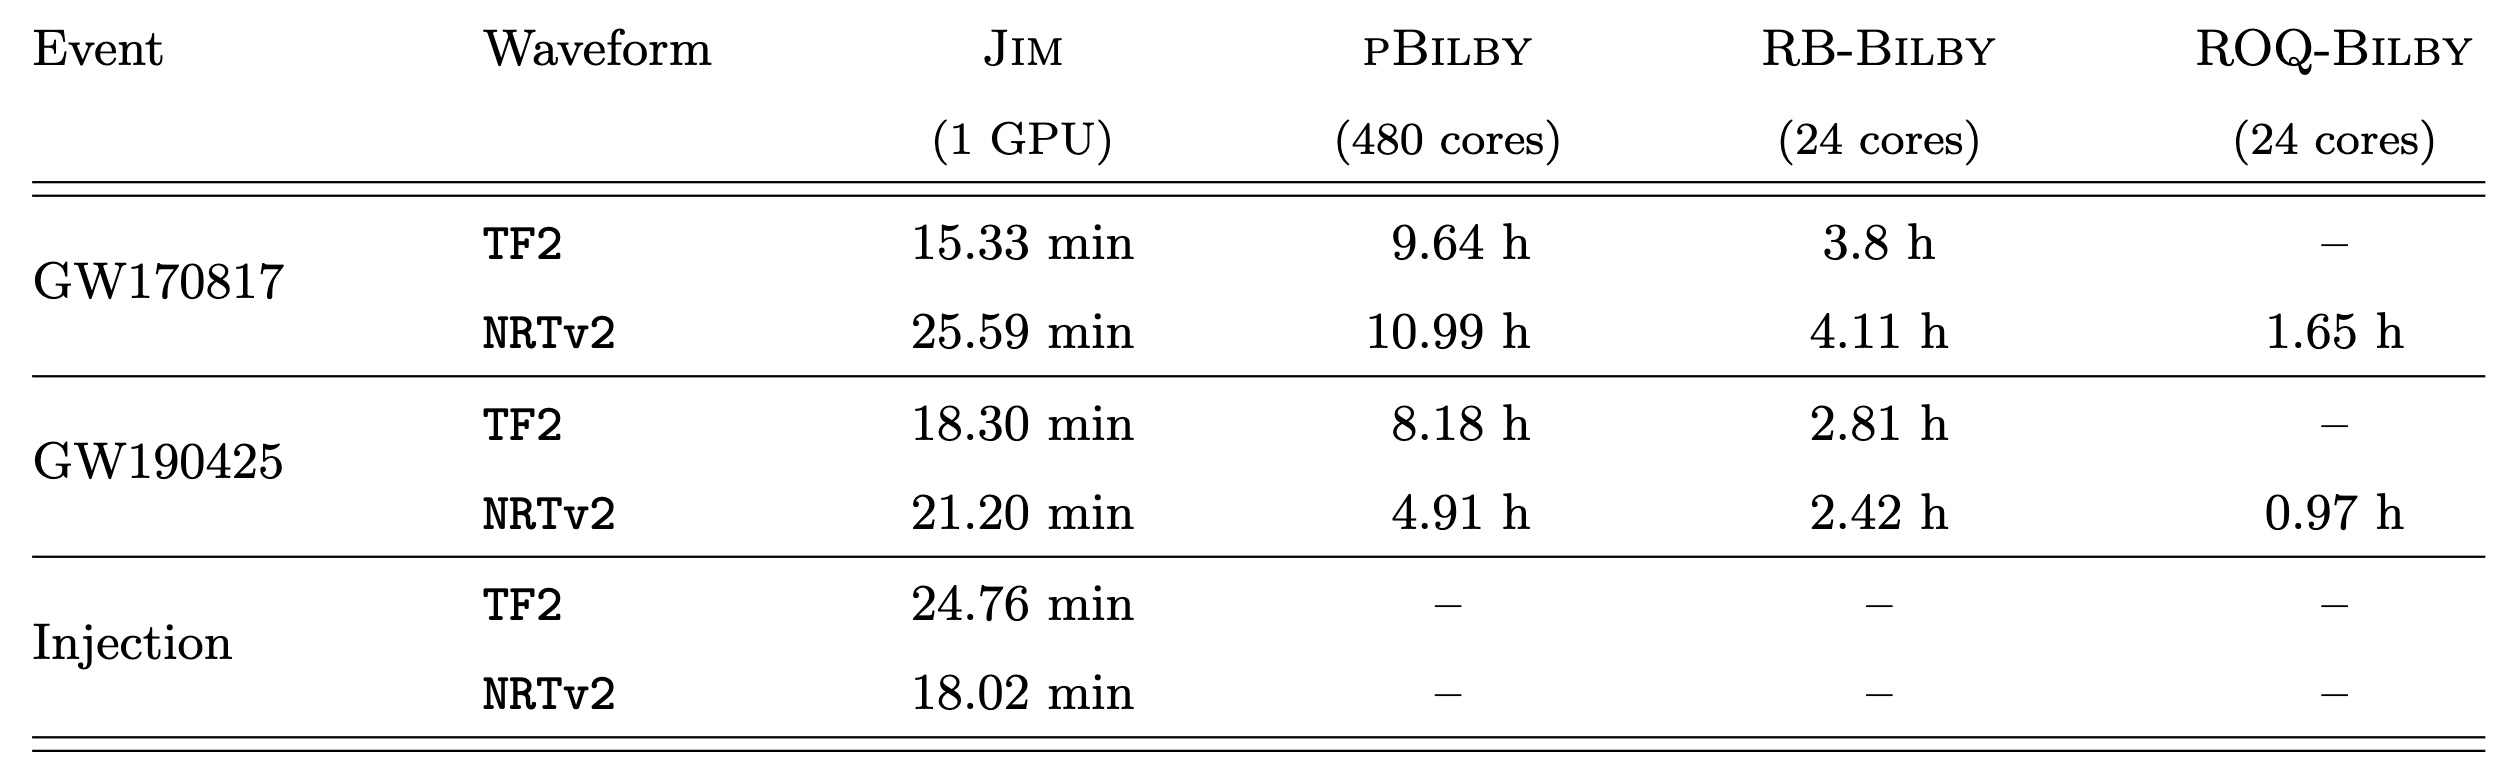
\includegraphics[width=0.95\linewidth]{Figures/jim_table_runtimes.jpg}
    \end{figure}
  }

  \vspace{\x}

  \only<3>{
    \begin{figure}
      \centering
      \includegraphics[width=0.80\linewidth]{Figures/Jim_ess.jpg}
    \end{figure}
  }

  \only<4>{
    \begin{figure}
      \centering
      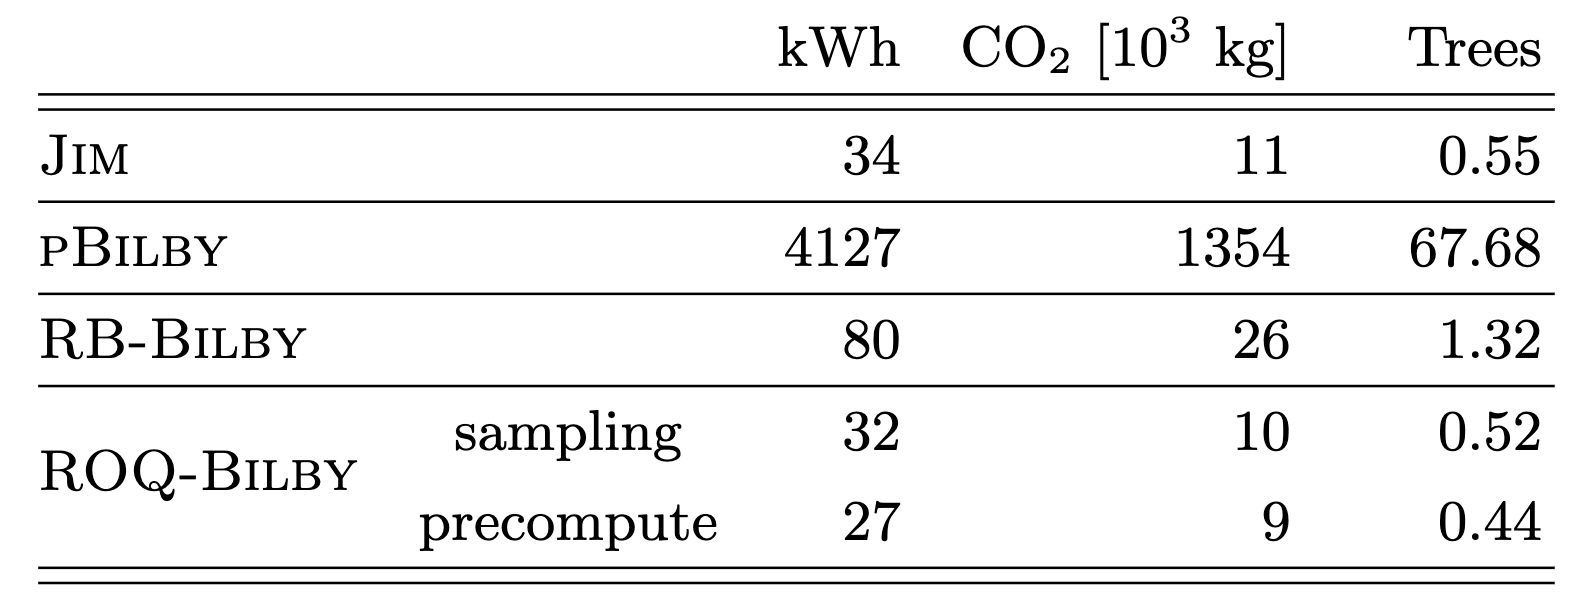
\includegraphics[width=0.80\linewidth]{Figures/Jim_trees.jpg}
    \end{figure}
  }

\end{frame}

% \begin{frame}{Gravitational waves: GWTC-3 analysis -- Thomas Ng}

%   \begin{itemize}
%     \item Re-analyze GWTC-3 with \texttt{IMRPhenomPv2}
    
%     \pause

%     \item \textsc{Jim} on A800 GPU: on average $\sim 7$ times faster than \textsc{bilby} on 16 CPUs, \textbf{without compromises}
    
%     \item \red{Work in progress!}
%   \end{itemize}

%   \vspace{2mm}

%   \begin{figure}
%     \centering
%     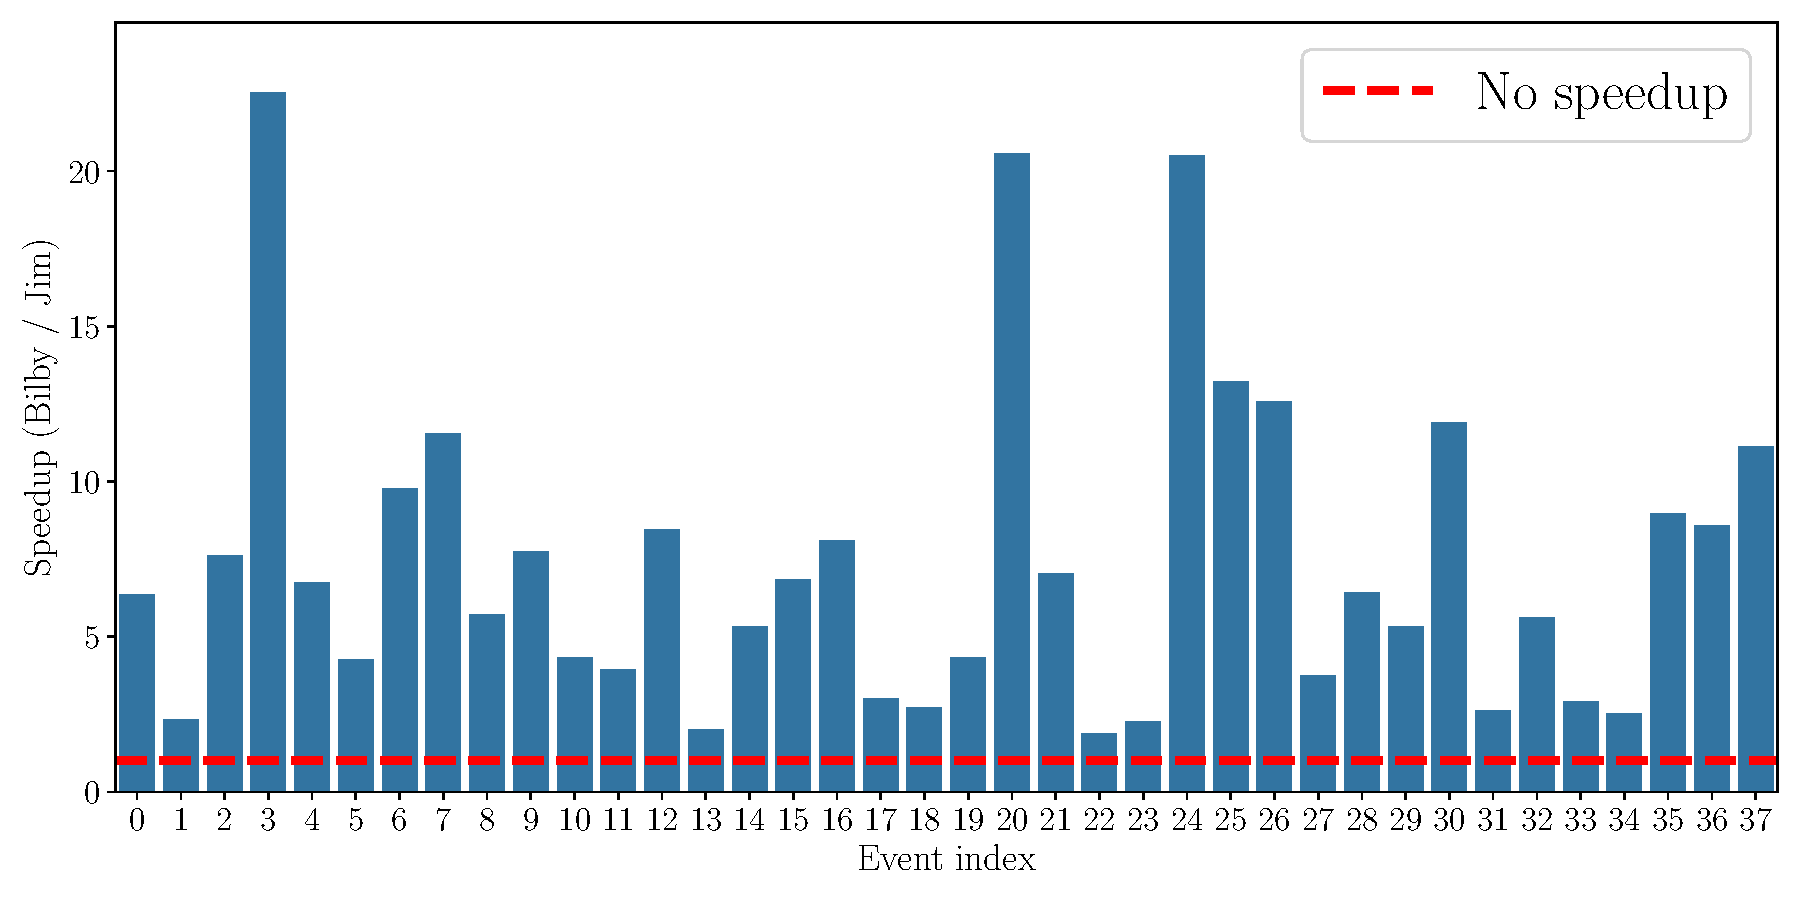
\includegraphics[width=0.90\linewidth]{Figures/speedup_NVIDIA_A800-SXM4-80GB.pdf}
%   \end{figure}
  
% \end{frame}


\begin{frame}{Einstein Telescope}

  \def\x{4mm}

  \begin{tcolorbox}[colback=red!10!white, colframe=red!80!black, coltext=black]
  Work in progress: showing proof-of-concepts!
  \end{tcolorbox}

  \pause
  \vspace{2mm}

  \begin{columns}
    \begin{column}[t]{0.50\linewidth}
      \begin{itemize}
        \item ET posteriors are multimodal

        \vspace{\x}
        
        \item Normalizing flows help to jump between modes
      \end{itemize}
    \end{column}

    \begin{column}[t]{0.49\linewidth}
      \begin{figure}
        \centering
        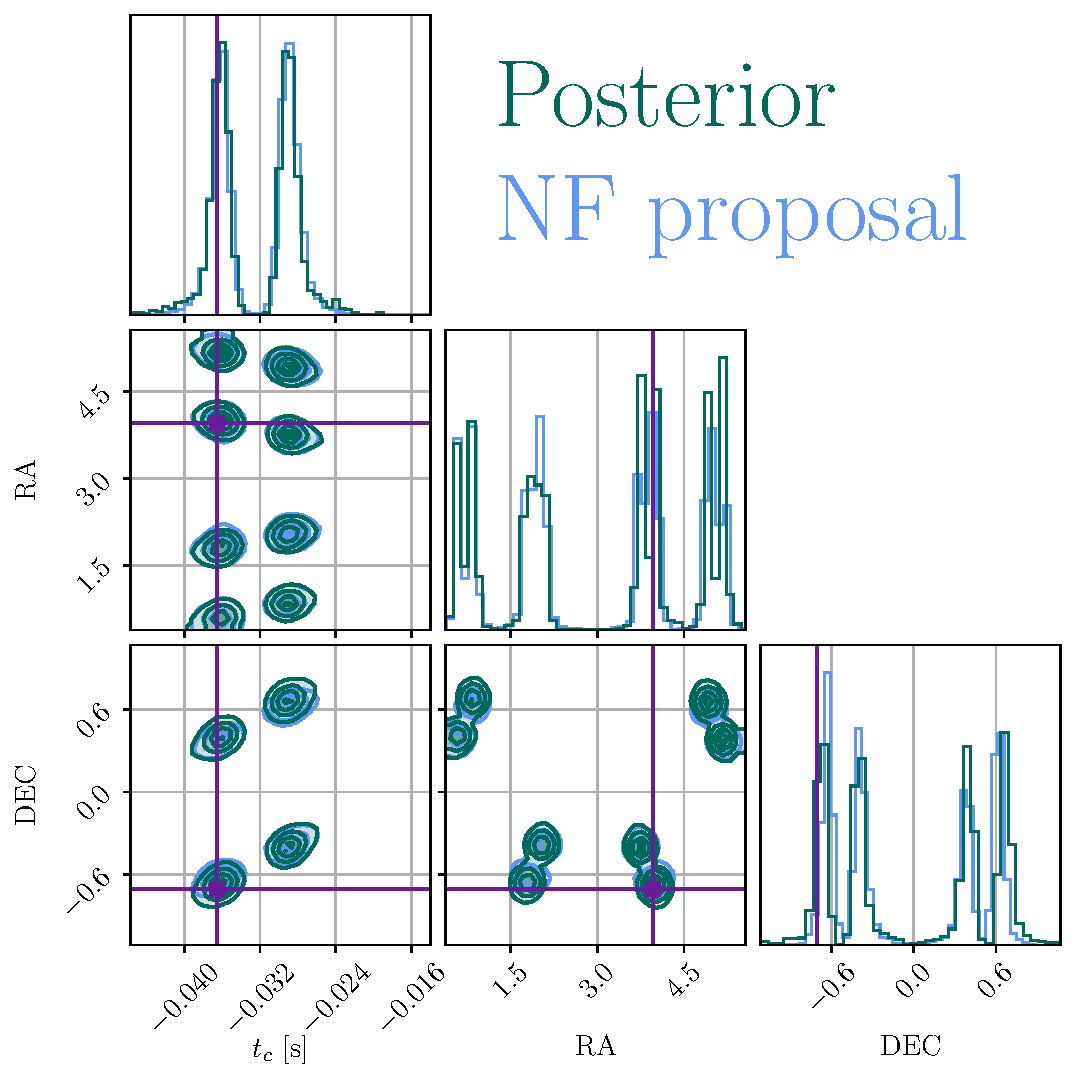
\includegraphics[width=0.90\linewidth]{Figures/corner_plot.pdf}
      \end{figure}
    \end{column}
  \end{columns}
\end{frame}

\begin{frame}{Overlapping signals}

  \def\x{1mm}

  %%% Colors used in case needed later on?
  % jax_BLUE = "#2a56c6" # jax blue, darker
  % jax_GREEN = "#00695c" # jax green, darker
  % jax_PURPLE = "#6a1b9a" # jax purple, darker

  % https://github.com/ThibeauWouters/jim_testing/tree/9ff1d374c3fa50f95ded8c2446a579c5f22cbb52/overlapping/HLV_BBH_BBH/outdir/injection_139_v2

  %%% For injection_139_v2, the parameters are: 
  % M_c_1 = 32.06485311503819, M_c_2 = 33.41456227648163

  \begin{itemize}
    % \item In 3G, we expect to see \red{overlapping signals}
    
    \item Assess scaling of \textsc{Jim}: \jaxbluedark{BBH}+\jaxgreendark{BBH} with LIGO-Virgo
    \begin{itemize}
      \vspace{\x}
      \item 2 binary black hole mergers: $22$ parameters

      \vspace{\x}

      \item $\jaxbluedark{M_c^{(1)}} = 32 M_\odot$, $\jaxgreendark{M_c^{(2)}} = 33 M_\odot$, $\Delta t = 70$ ms
      
      \vspace{\x}

      \item $\jaxbluedark{\rm{SNR}^{(1)}} = 25.76$, $\jaxgreendark{\rm{SNR}^{(2)}} = 25.24$ 

      \vspace{\x}

      \item $1$h$28$m on H100 GPU (vs several days on 16 CPUs~\cite{Janquart:2022fzz})
    \end{itemize}
  \end{itemize}

  \vspace{-4mm}
  
  \begin{columns}
    \begin{column}{0.49\textwidth}
      \begin{figure}
        \centering
        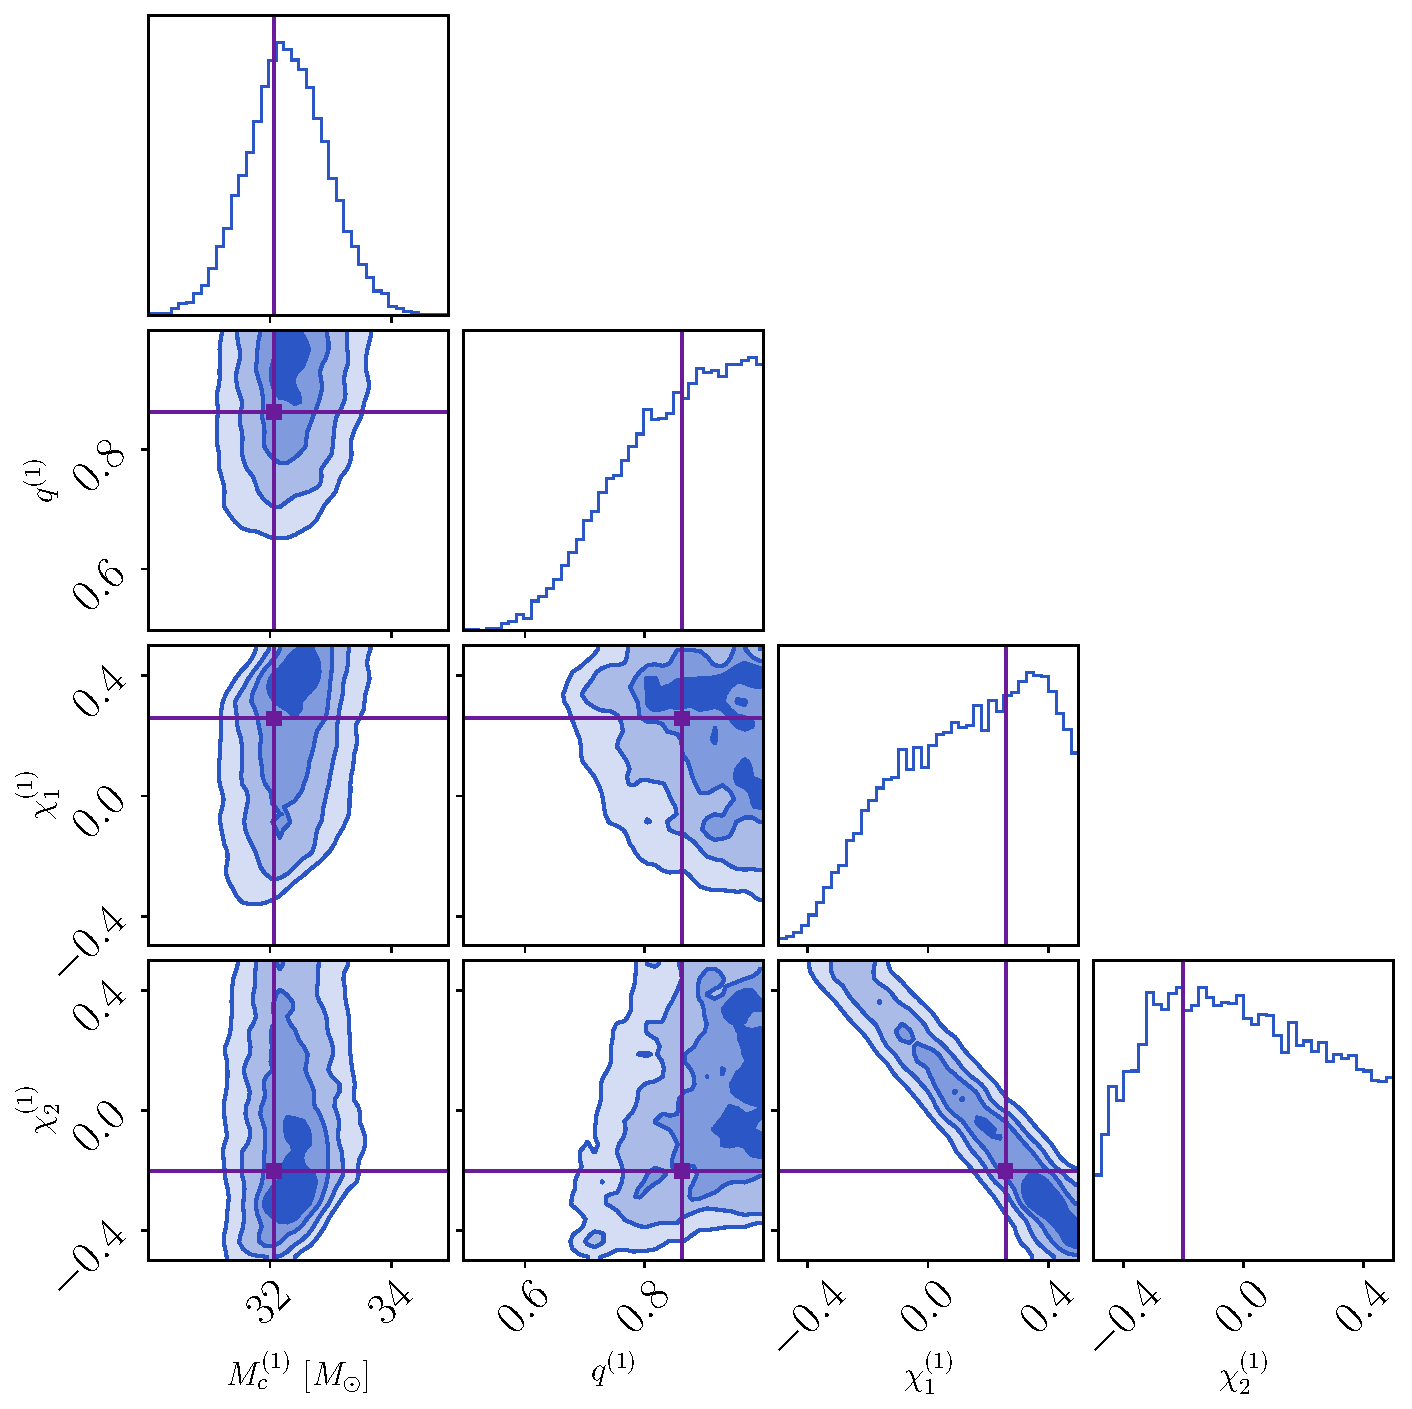
\includegraphics[width=0.85\linewidth]{Figures/OS_injection_139_v2_1_cornerplot_M_c_q_s1_z_s2_z.pdf}
      \end{figure}
    \end{column}

    \begin{column}{0.49\textwidth}
      \begin{figure}
        \centering
        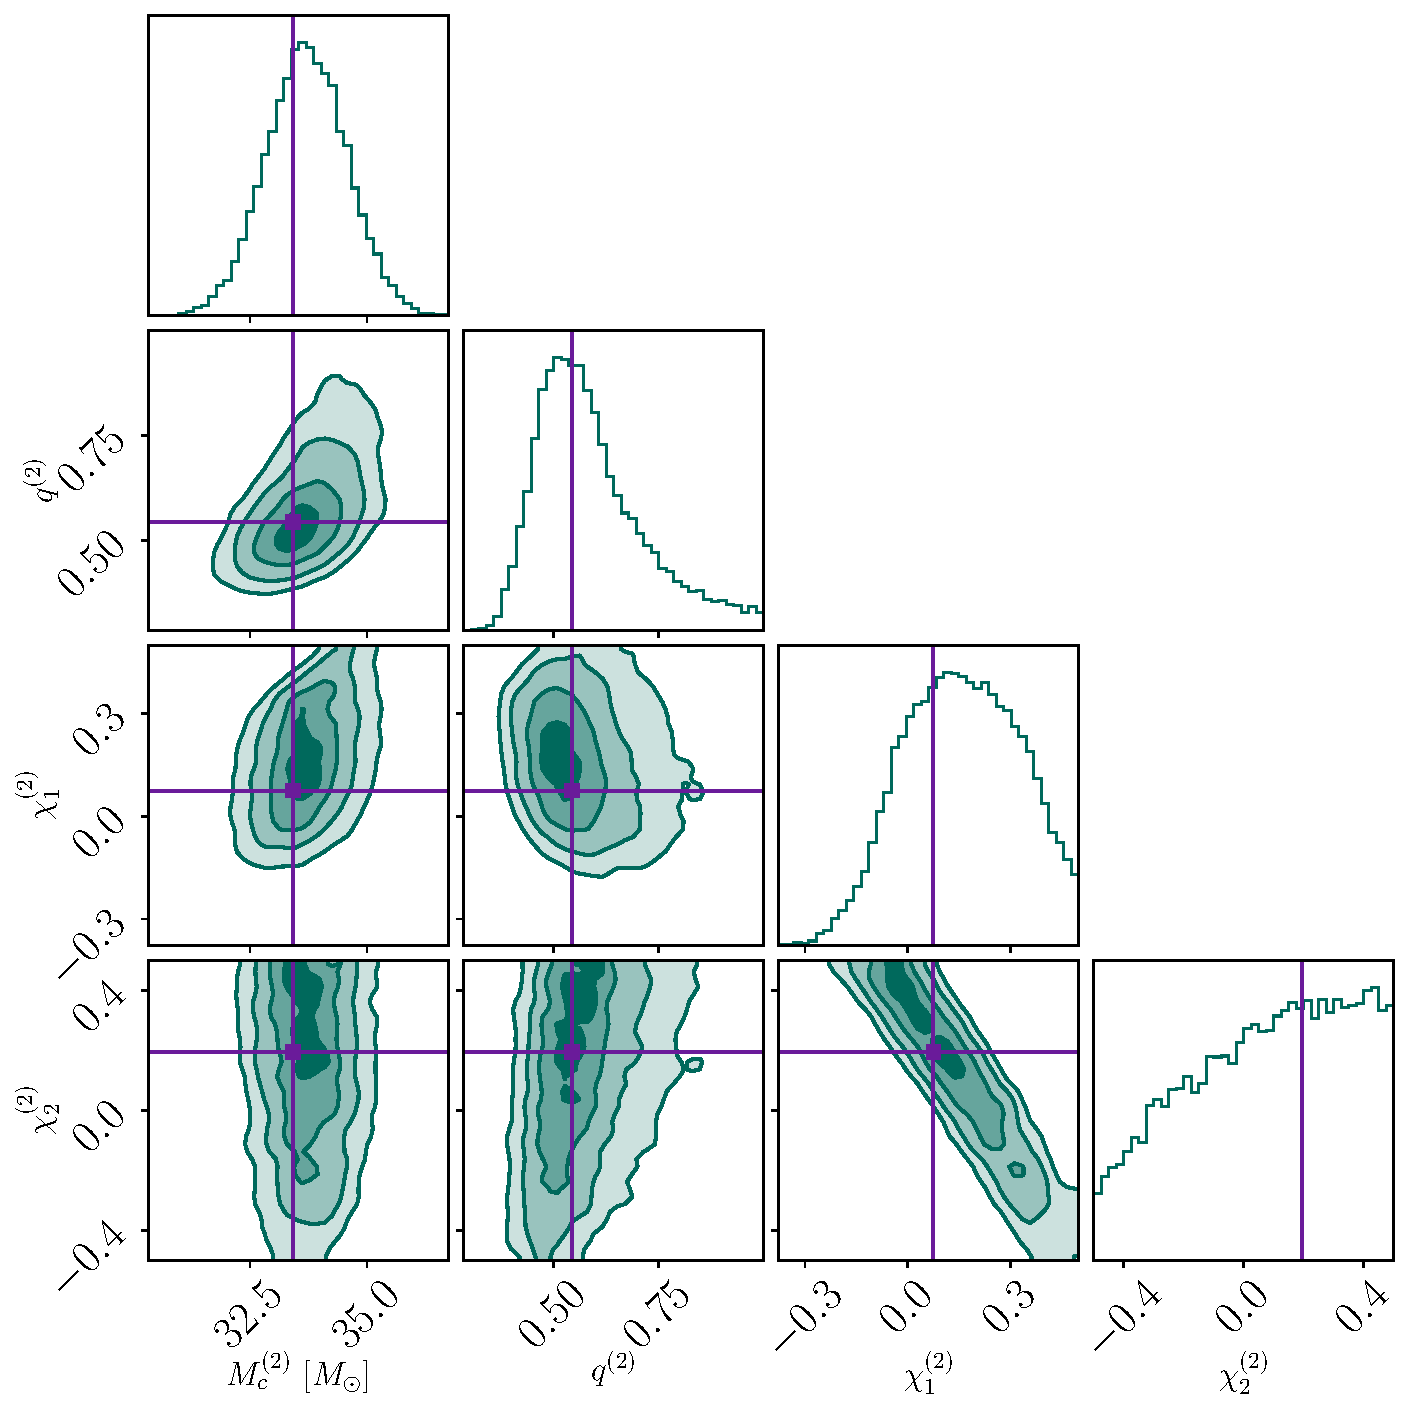
\includegraphics[width=0.85\linewidth]{Figures/OS_injection_139_v2_2_cornerplot_M_c_q_s1_z_s2_z.pdf}
      \end{figure}
    \end{column}
  \end{columns}
\end{frame}

\begin{frame}{Open call}

  \begin{itemize}
    \item Biggest bottleneck in development: \textsc{JAX} waveforms

    \vspace{3mm}
    
    \item Most waveforms developed in C, some waveforms in Python 
    
    \vspace{3mm}
    
    \item What is the reason \textit{not} to go for \textsc{JAX}?
  \end{itemize}

  \vspace{10mm}
  \pause 

  \begin{tcolorbox}[colback=green!10!white, colframe=green!80!black, coltext=black]
  Get in touch if you are interested! We need you!

  \vspace{3mm}

  \textsc{Jim} developers $\cap$ waveform developers = \textbf{you}?
  \end{tcolorbox}

  \vspace{10mm}
  
\end{frame}

\begin{frame}[plain, noframenumbering]{Overview}
  \showoverview{2}
\end{frame}

\begin{frame}{Electromagnetic counterparts \small (Hauke Koehn)\normalsize}
  \def\x{2mm}

  \begin{itemize}
    \item Predicting a \red{GRB afterglow} is slow

    \vspace{\x}
    
    \item Code libraries too large to `jaxify': neural network emulators for inference: \textsc{fiesta}~\ghlink{nuclear-multimessenger-astronomy/fiestaEM}~\cite{Koehn:2025zzb}
      
    \vspace{\x}

    \item<2-> Scales well for systematics `nuisance parameters'
  \end{itemize}

  \onslide<1->{
    \begin{columns}
      \begin{column}[c]{0.14\textwidth}
        \centering
        \incfig[0.90\textwidth]{GRB}
      \end{column}
  
      \begin{column}[c]{0.24\textwidth}

        \vspace{-5mm}

        \fiesta{\textsc{fiesta}}
        \begin{itemize}
          \item $1$m$36$s
          \item $1$ H100 GPU
        \end{itemize}
        
        \vspace{6mm}

        \afterglowpy{\textsc{afterglowpy}}
        \begin{itemize}
          \item $4$ hours
          \item $30$ CPUs
        \end{itemize}
      \end{column}
  
      \begin{column}[c]{0.59\textwidth}
        \only<1>{
          \begin{figure}
          \centering
          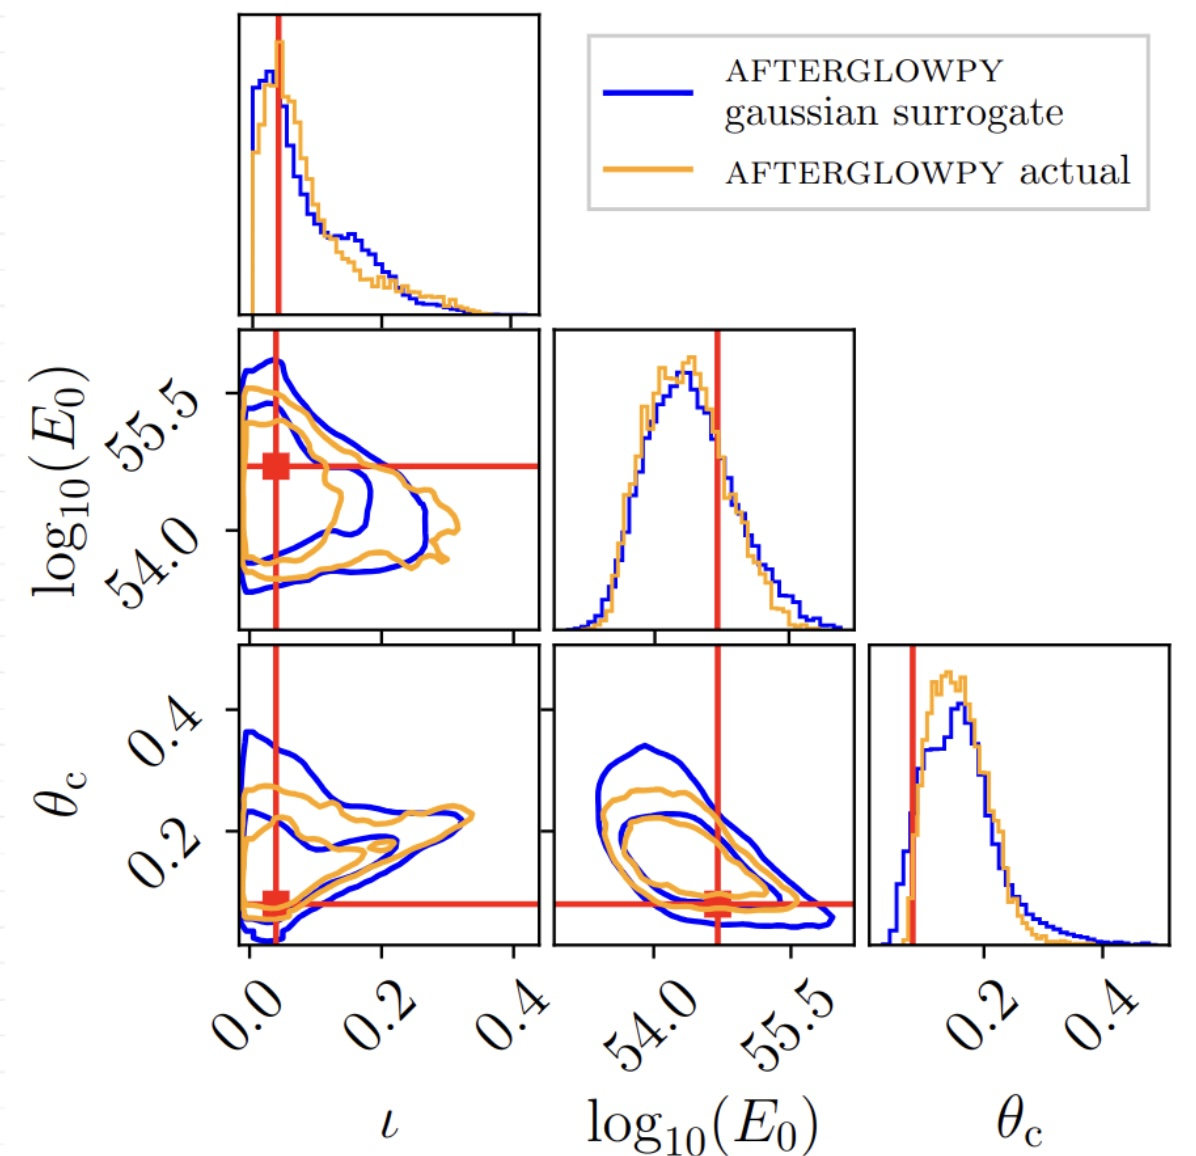
\includegraphics[width=0.70\linewidth]{Figures/fiesta_result.jpg}
        \end{figure}
        }
        \only<2>{
          \vspace{2mm}
          \begin{figure}
          \centering
          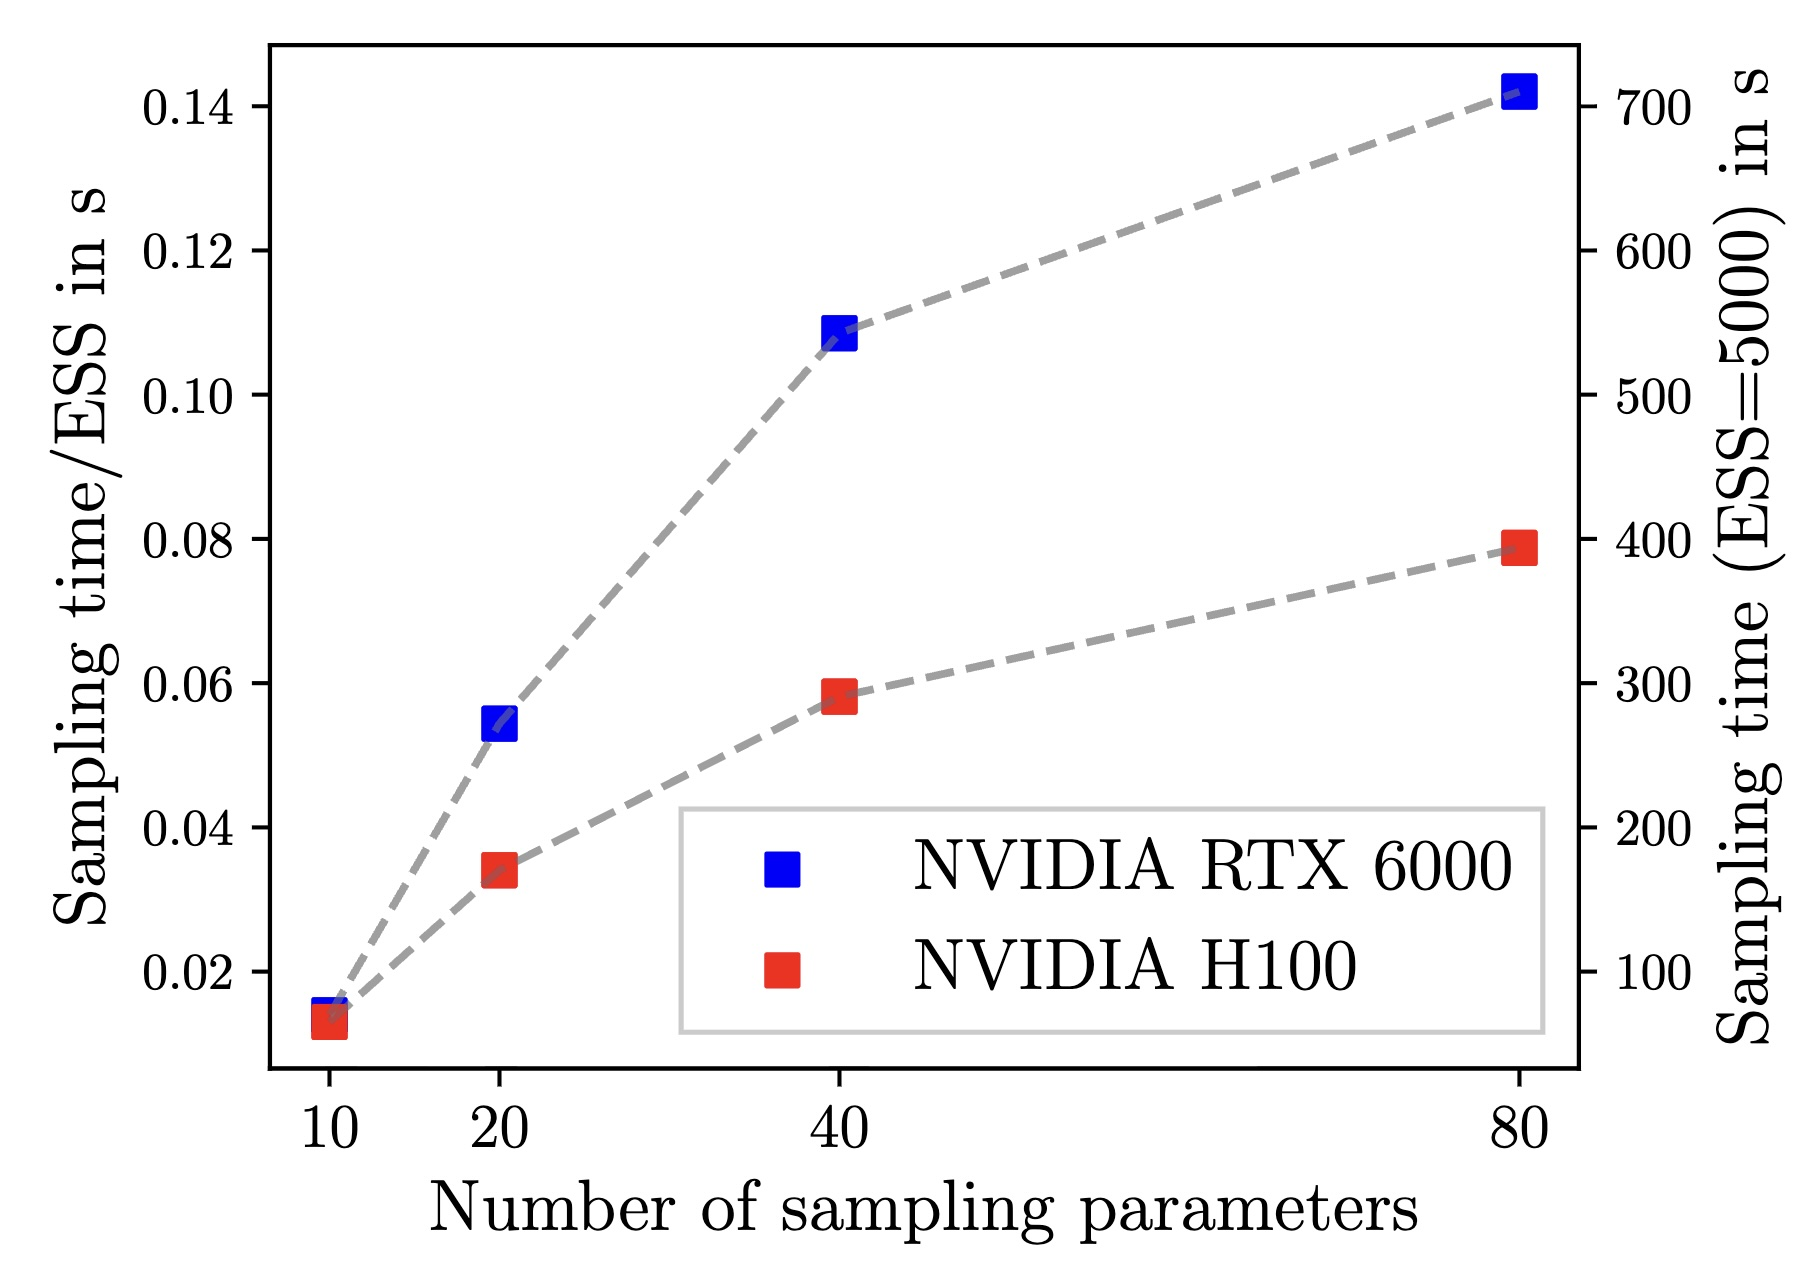
\includegraphics[width=0.825\linewidth]{Figures/fiesta_scaling.jpg}
        \end{figure}
        }
      \end{column}
    \end{columns}
  }
\end{frame}

\begin{frame}{Overview}
  \showoverview{3}
\end{frame}

\begin{frame}{Equation of state inference -- warmup}

  \def\x{3mm}
  \def\y{3mm}

  \begin{itemize}
    \item How do we constrain the EOS from neutron star observations?

    \vspace{\y}
    
    \item Define parametrization and likelihood
    
    % \vspace{\y}
    
    % \item GWs from binary neutron stars inspiral as example
  \end{itemize}

  \vspace{\x}
  
  \centering
  \begin{figure}
    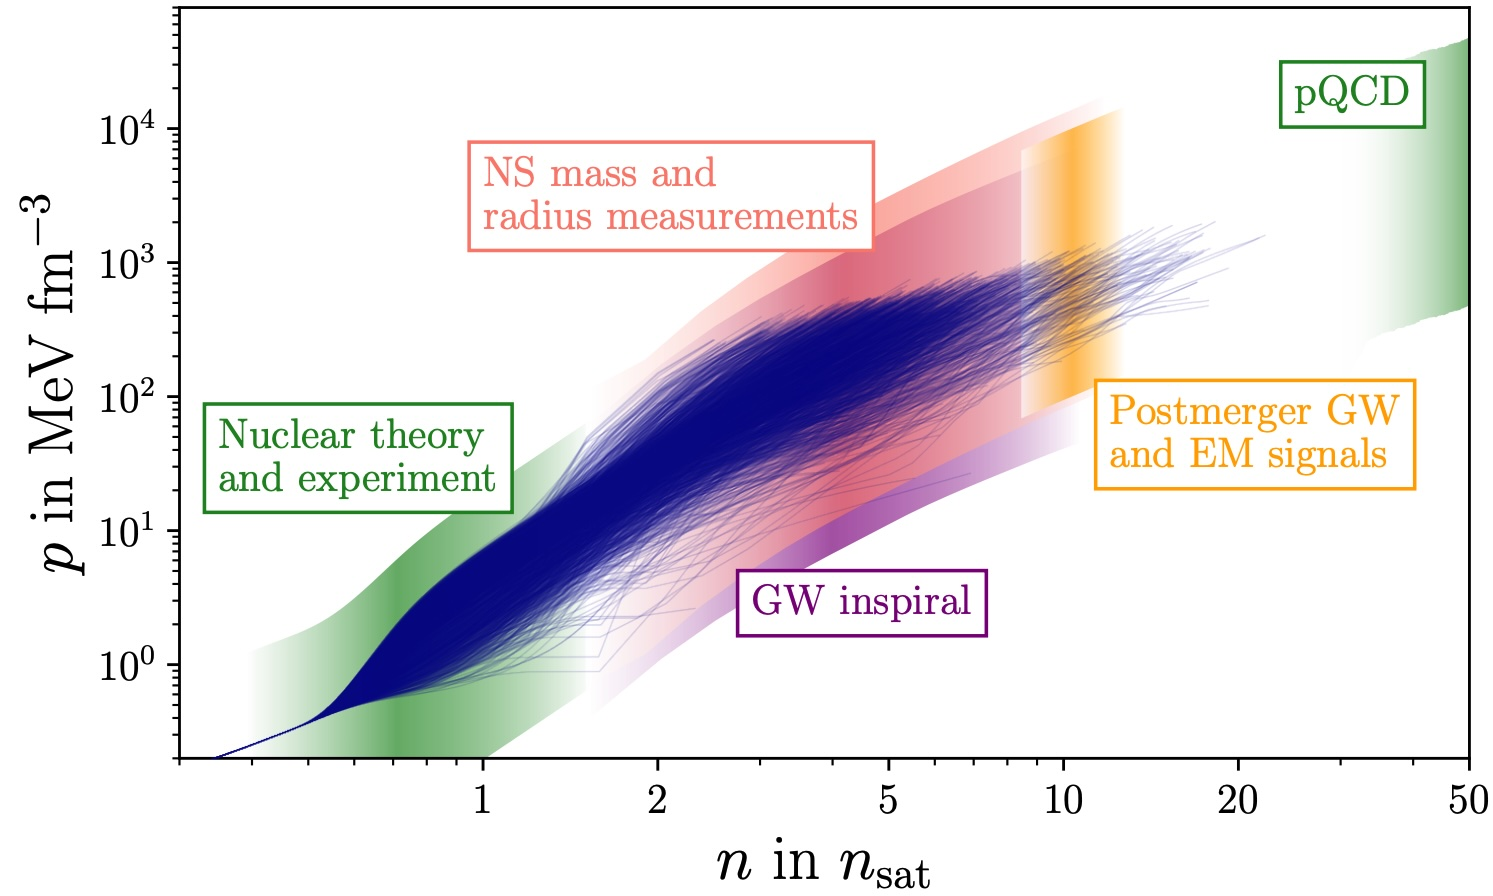
\includegraphics[width=0.75\linewidth]{Figures/Koehn_EOS.jpg}
  \end{figure}
  
\end{frame}

\begin{frame}{Equation of state inference -- parametrization}

  \def\x{2mm}
  \def\y{1mm}

  \begin{itemize}
    \item $n \leq \tfrac12 n_{\rm{sat}}$: fixed crust

    \vspace{\x}
    
    \item $\tfrac12 n_{\rm{sat}} \leq n \leq \red{n_{\rm{break}}}$: metamodel EOS, nuclear physics inspired
    
    \vspace{\x}

    \item $n \leq \red{n_{\rm{break}}}$: agnostic extension

    \vspace{\x}

    \item $>26$ (\textbf{!}) parameters $\thetaeos$
  \end{itemize}

  \centering
  \incfig[0.825\textwidth]{EOS_parametrizion}
\end{frame}

\begin{frame}{Tidal deformability}
  \def\x{4mm}

  \begin{itemize}
    \item Neutron stars are tidally deformed in a binary, quantified by tidal deformability $\Lambda$: affect phase of GWs
    
    \vspace{\x}
    
    \item Neutron stars: $\Lambda = \Lambda(m, \rm{EOS})$, black holes: $\Lambda = 0$
    
    % \vspace{\x}

    % \item Black holes: $\Lambda = 0$

    \vspace{\x}

    \item GWs give us $p(m_1, m_2, \Lambda_1, \Lambda_2 | d)$ for EOS inference
  \end{itemize}

  \vspace{\x}

  \centering
  \incfig[1.0\textwidth]{tidal}
\end{frame}

% \begin{frame}{Tidal deformability postprocessing}

%   \def\x{3mm}

%   \begin{itemize}
%     \item Binary neutron star GWs: $17$ parameters

%     \vspace{\x}

%     \item EOS: only need masses and tidal deformabilities

%     \vspace{\x}

%     \item Marginal $4$d posterior: obtained with normalizing flow
%   \end{itemize}

%   \vspace{\x}

%   \begin{figure}
%     \centering
%     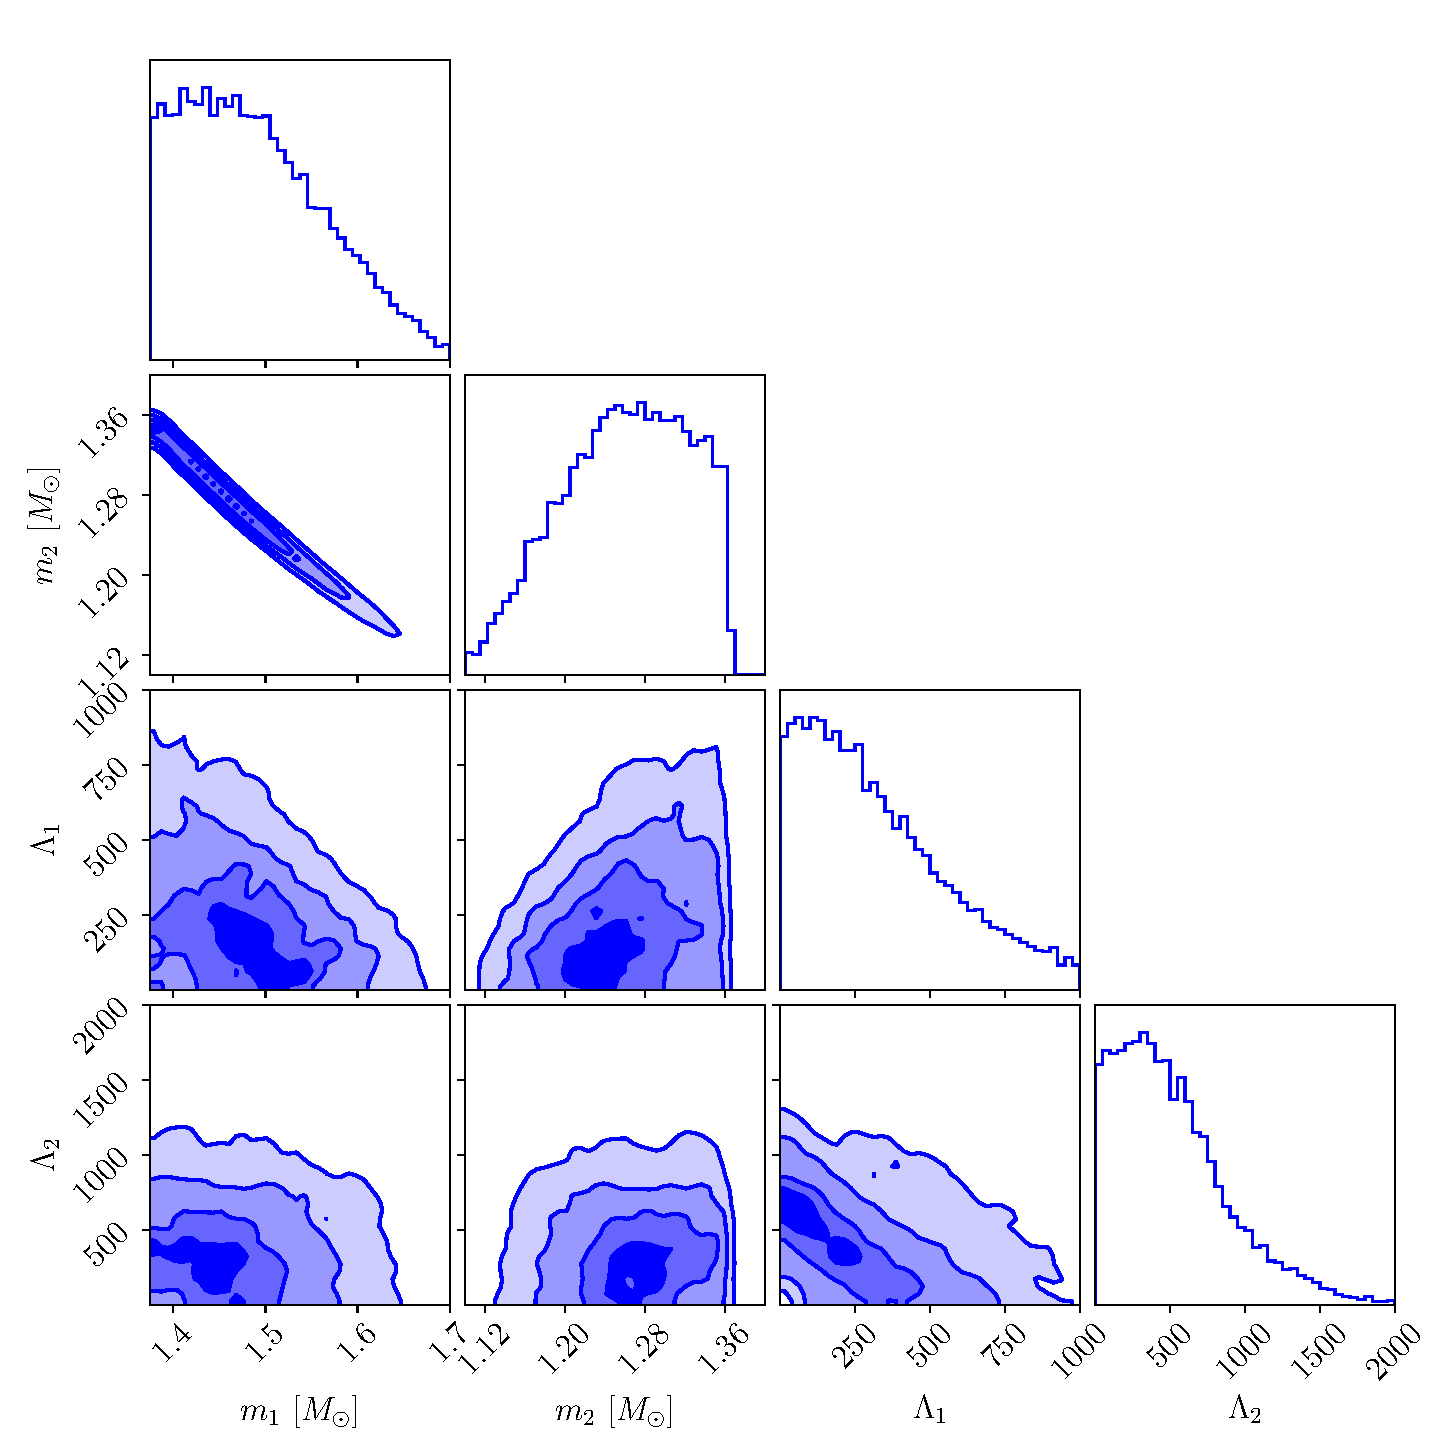
\includegraphics[scale=0.225]{Figures/GW170817_mass_lambdas_plot.pdf}
%   \end{figure}

%   % \centering
%   % \incfig[0.95\textwidth]{GW170817_mass_lambdas}

% \end{frame}

\begin{frame}{Equation of state}
  \def\x{2mm}
  \def\y{5mm}

  \begin{itemize}
    \item To predict neutron star properties, we solve the TOV equations: ordinary differential equations (ODEs)
    
    \vspace{\x}

    \item<2-> Done for each sample $\theta_{\rm{EOS}}$: \red{costly likelihood}
    
    \vspace{\x}

    \item<2-> How to make this scalable without compromises?
  \end{itemize}

  \vspace{\y}

  \only<1>{
    \centering
    \incfig[0.95\textwidth]{TOV}
  }

  \only<2->{
    \centering
    \incfig[0.95\textwidth]{NS_likelihood}
  }

\end{frame}

\begin{frame}{\textsc{Jester}}
  \def\x{2mm}

  \begin{itemize}
    \item \textsc{Jester}~\ghlink{nuclear-multimessenger-astronomy/jester}~\cite{Wouters:2025zju}: \textsc{jax}-based TOV solver
    \begin{itemize}
      \item $1000\times$ faster, without compromises
      \item Full inference in \red{$\sim$hours}
    \end{itemize}

    \vspace{\x}

    \item<2-> \textsc{Jim}$+$\textsc{Jester}: from GWs to EOS in a few hours
    \begin{itemize}
      \item Example: 20 binary neutron stars in O5
    \end{itemize}

    \vspace{\x}
    
    \item<2-> Enable systematics studies in EOS inference
  \end{itemize}

  \vspace{-3mm}

  \begin{columns}
    \onslide<1->{
      \begin{column}{0.49\textwidth}
        \begin{figure}
          \centering
          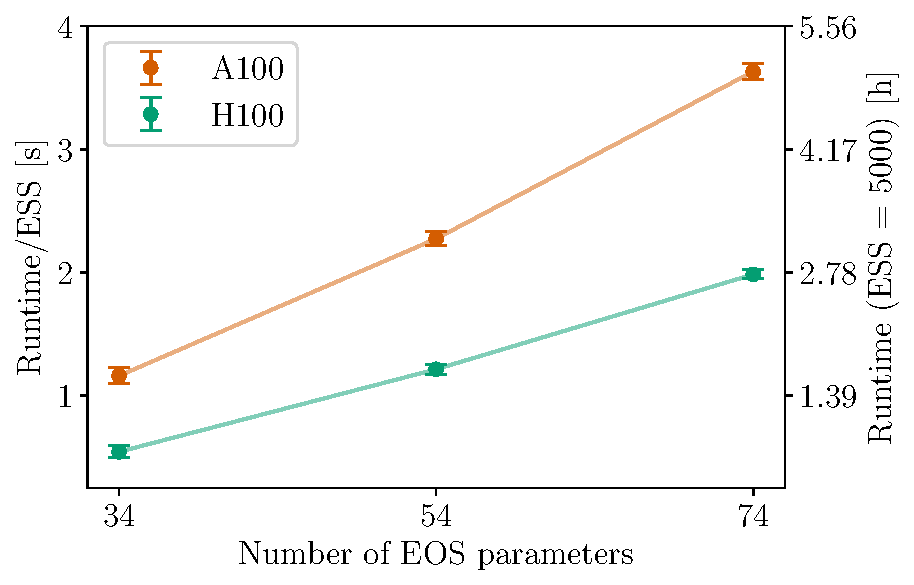
\includegraphics[width=0.99\linewidth]{Figures/scaling_plot.pdf}
        \end{figure}
      \end{column}
    }

    \onslide<2->{
      \begin{column}{0.475\textwidth}
        \begin{figure}
          \centering
          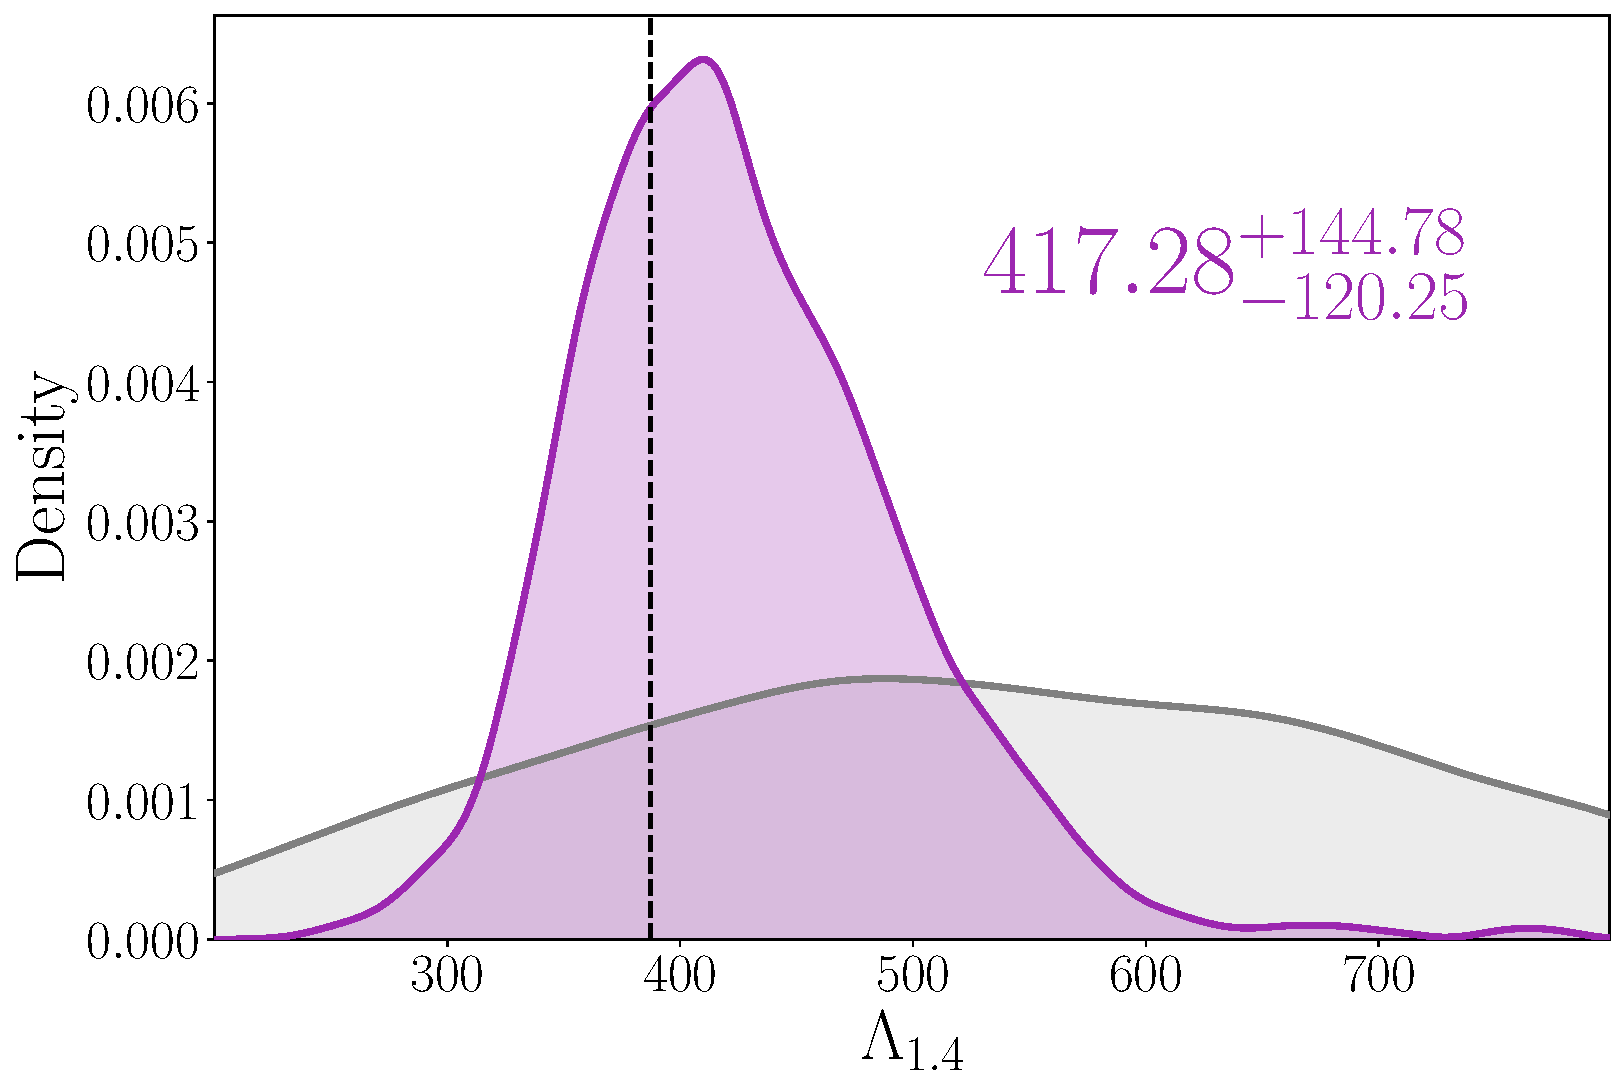
\includegraphics[width=0.99\linewidth]{Figures/BNS_EOS_projection.pdf}
        \end{figure}
      \end{column}
    }
  \end{columns}
\end{frame}

\begin{frame}{Anistropy in neutron stars \small (Peter T. H. Pang) \normalsize}

  \def\x{1mm}

  \begin{itemize}
    \item Anistropic pressure: $\gamma \propto p - p_t$

    \vspace{\x}
    
    \item<2-> Magnetic fields, dark matter clusters, superfluids...

    \vspace{\x}
    
    \item<3-> Preference for negative anisotropy, but weak evidence~\cite{Pang:2025fes}
  \end{itemize}

  \begin{columns}
    \begin{column}{0.475\textwidth}
      \begin{figure}
        \centering
        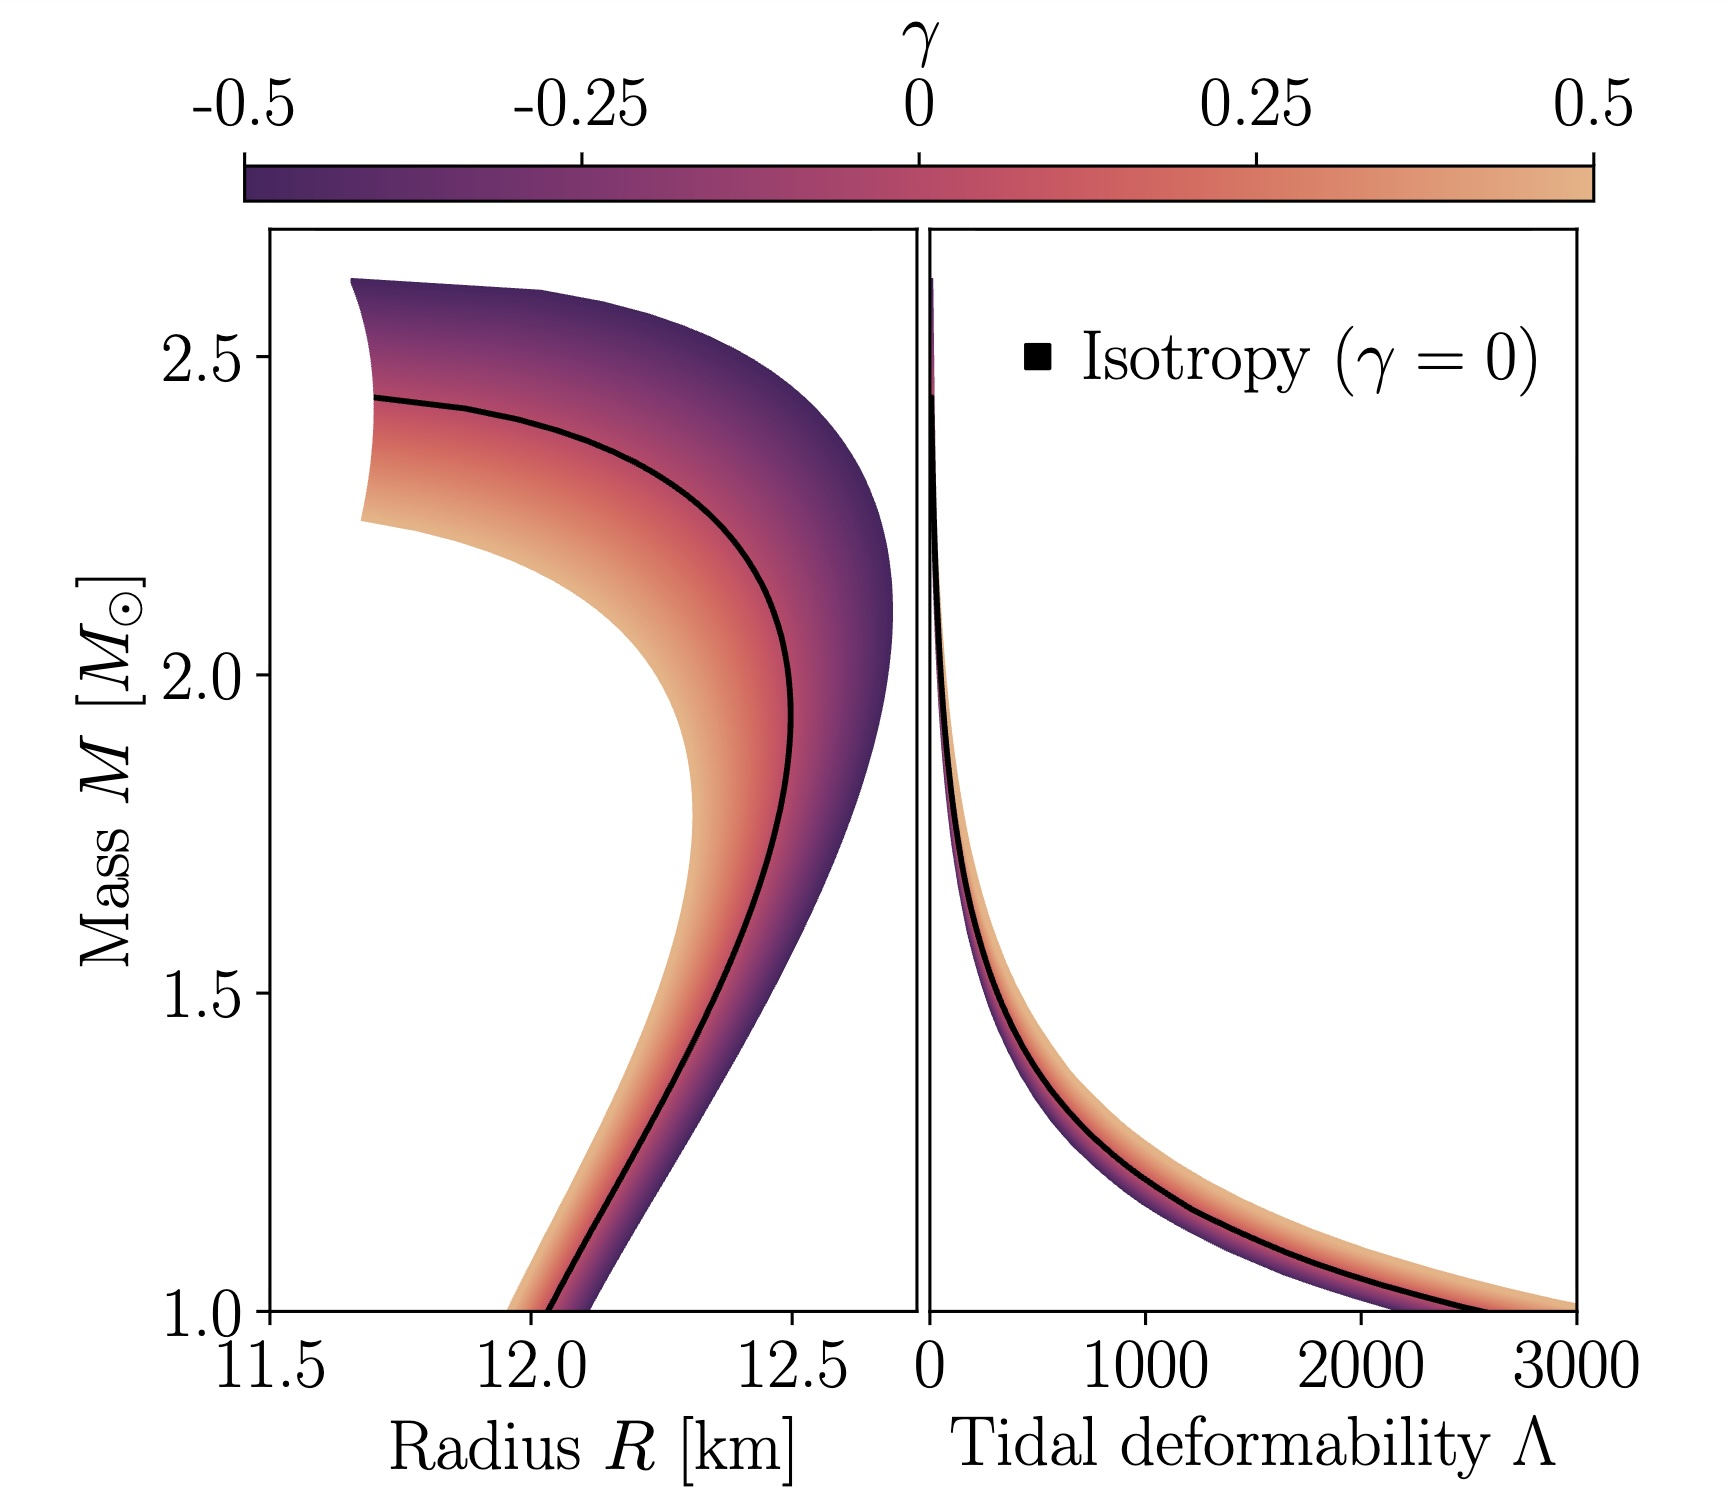
\includegraphics[width=0.99\linewidth]{Figures/anisotropy.jpg}
      \end{figure}
      
    \end{column}
    
    \begin{column}{0.475\textwidth}
      \onslide<3->{
        \begin{figure}
        \centering
        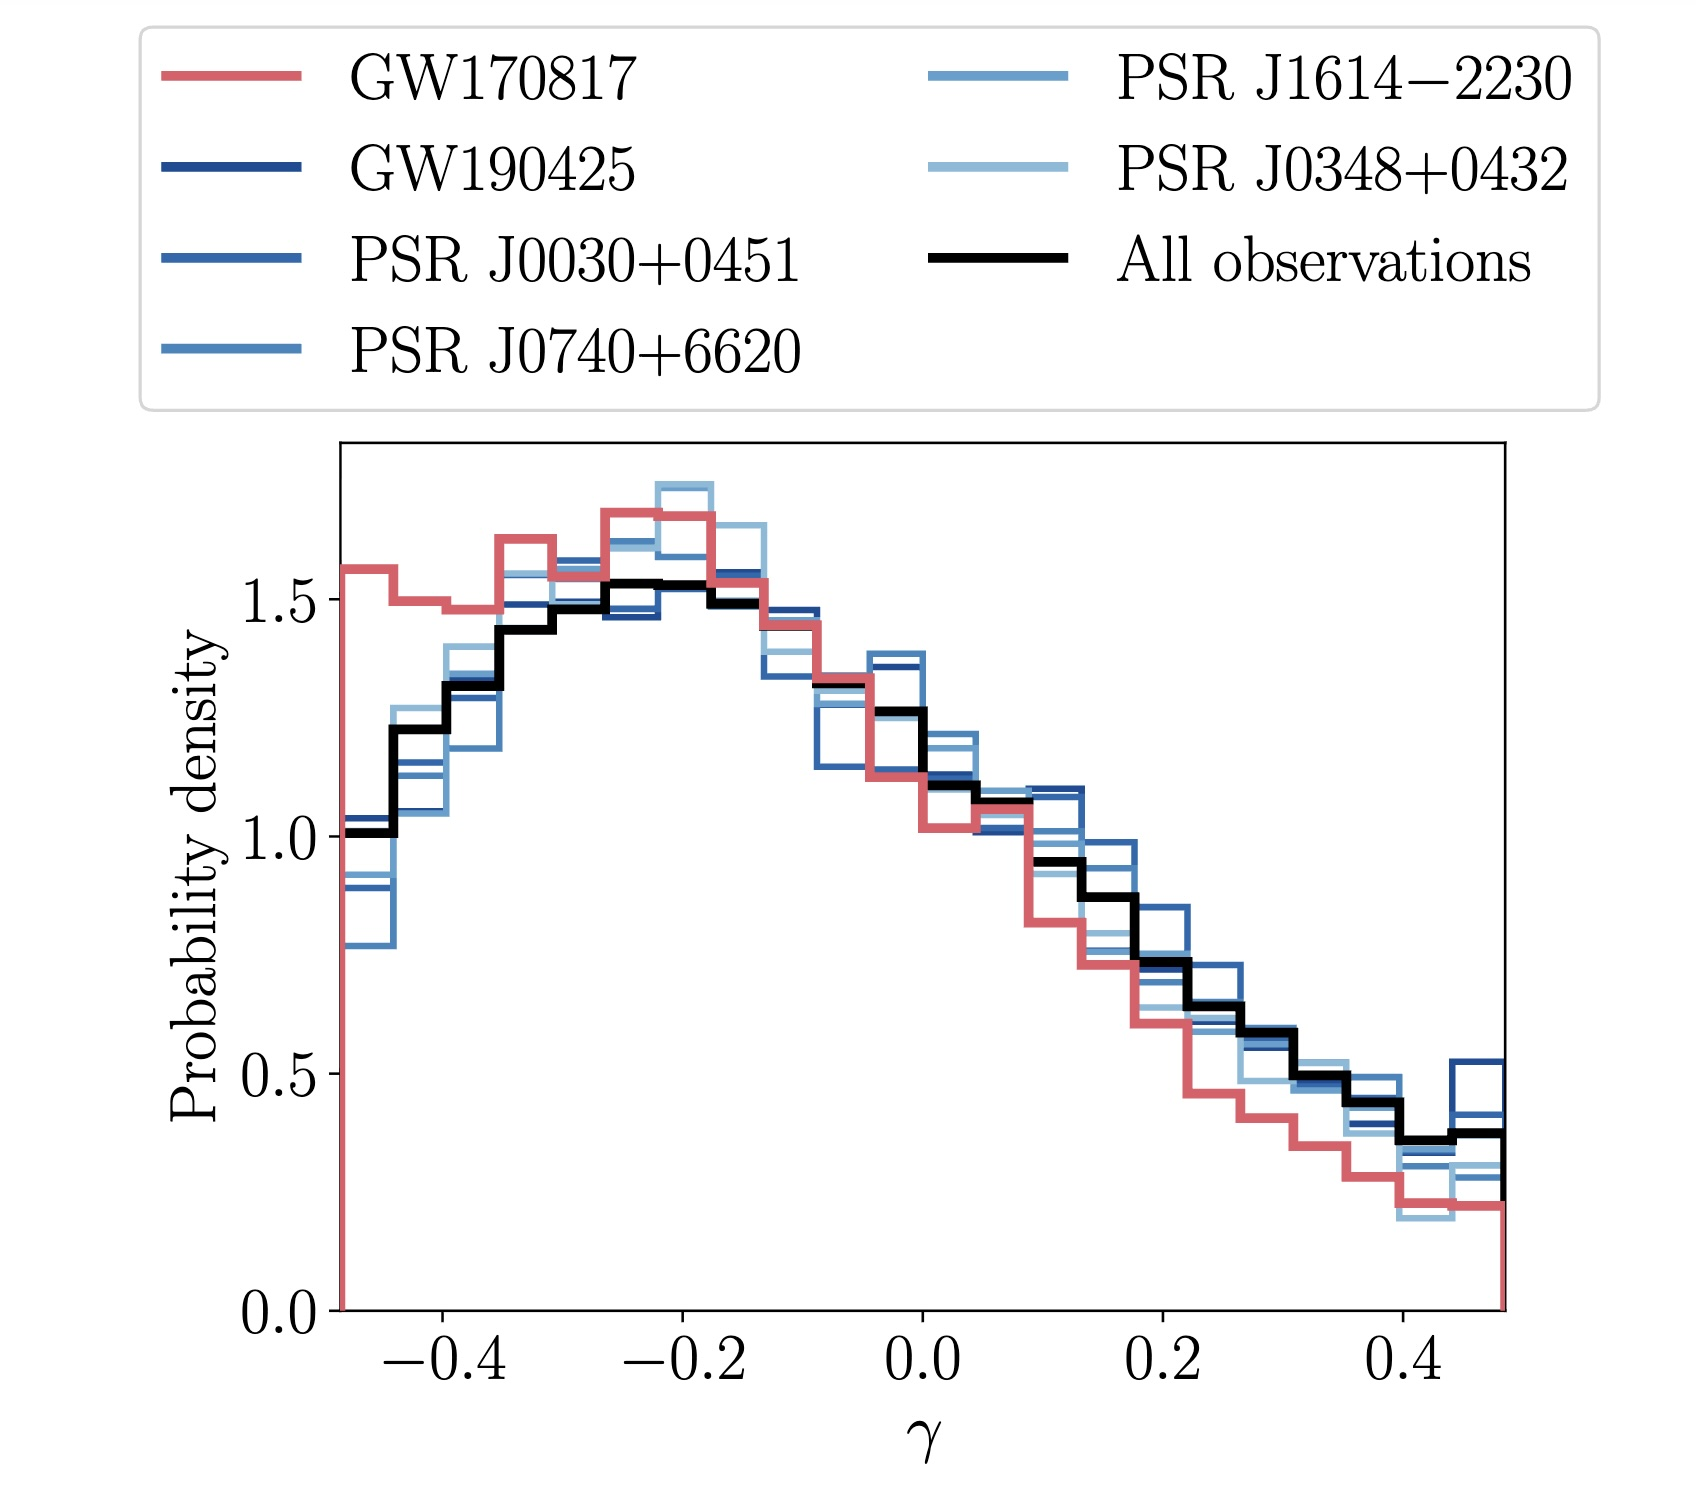
\includegraphics[width=0.99\linewidth]{Figures/measure_anistotropy.jpg}
      \end{figure}
      }
      
    \end{column}
  \end{columns}
  
\end{frame}

\begin{frame}{Auto-differentiable ODE solvers}

  \def\x{2mm}

  \begin{itemize}
    \item ODE solvers written in \textsc{jax} are auto-differentiable % (\textsc{diffrax}~\ghlink{patrick-kidger/diffrax})

    \vspace{\x}

    \item Frame inference as optimization problem:
    \begin{itemize}
      \item Gradient descent on loss function $\mathcal{L}(\thetaeos)$
    \end{itemize}
  \end{itemize}

  \vspace{3mm}

  \only<2->{
    \centering
    \incfig[0.95\textwidth]{jester_ad}
  }
\end{frame}

\section{Neural priors}

% \begin{frame}[plain]{}
%   \vspace{15mm}
%   \huge and now, for something completely different... \normalsize
%   \vspace{15mm}
% \end{frame}

\begin{frame}{Neutron star data analysis loop}

  \def\x{2mm}
  \def\y{3mm}

  Data analysis of neutron stars forms a \textbf{loop}:

  \vspace{1mm}
  \begin{enumerate}
      \item Constraining the EOS with neutron star observations

      \vspace{\x}
      
      \item \red{Applying} EOS knowledge in neutron star data analysis (e.g., GW)
  \end{enumerate}

  \vspace{\x}

  How can we efficiently perform \red{Step 2}?

  \vspace{5mm}

  \centering
  \incfig[0.9\textwidth]{NS_to_EOS}
\end{frame}

\begin{frame}{Case study}

  \def\x{2mm}
  \def\y{2mm}

  \begin{itemize}
    \item Take constraints on EOS from:
    \begin{itemize}
      \vspace{\y}
      \item \textbf{Radio timing}: EOS must support $2\,M_{\odot}$ neutron stars

      \vspace{\y}

      \item \textbf{Chiral EFT}: nuclear theory predictions (valid $<2 n_{\rm{sat}}$)
      
      \vspace{\y}

      \item \textbf{NICER}: Mass-radius observations of neutron stars
    \end{itemize}
  \end{itemize}
    
  \vspace{\x}
  \centering
  \incfig[0.85\textwidth]{R14_table}
  \vspace{\x}
    
  \begin{itemize}
    \item How can we use this information in GW analyses?
  \end{itemize}
\end{frame}


\begin{frame}{Equation of state-informed priors}
  \def\x{4mm}
  \def\y{1mm}

  \begin{itemize}
    \item This should enter the prior on $\Lambda_i$
    \begin{align*}
      \mathcal{P}(\theta_{\rm{GW}} | d ) &\propto \mathcal{L}(d | \theta_{\rm{GW}}) \red{\pi(\theta_{\rm{GW}})}
    \end{align*}

    % \vspace{-4mm}

    \item By default, we choose \textbf{\jaxthree{agnostic priors}}: e.g. $\Lambda_{1,2} \sim \mathcal{U}(0, 5000)$

    \vspace{\x}
    \pause

    \item \textbf{But}, we have prior knowledge from the EOS:
    \begin{itemize}
      \vspace{\y}
      \item Masses $m_i$ determined by $M_{\rm{max}}$ (or population)

      \vspace{\y}

      \item $\Lambda_i = \Lambda_i(m_i, {\rm{EOS}})$
    \end{itemize}
    
    \vspace{\x}
    \pause
    
    \item \textbf{\jaxtwo{Equation of state-informed prior}}: take \jaxtwo{EOS uncertainty} into account
    \begin{align*}
      \pi(m_1, m_2, \Lambda_1, \Lambda_2) = \int \diff \theta_{\rm{EOS}} \ &\pi(m_1, m_2 | \theta_{\rm{EOS}}) \pi(\Lambda_1, \Lambda_2 | m_1, m_2, \theta_{\rm{EOS}}) \\
      &\times \jaxtwo{\pi(\theta_{\rm{EOS}})}
    \end{align*}
  \end{itemize}
\end{frame}


\begin{frame}{Equation of state-informed priors}
  \def\x{2mm}
  \def\y{2mm}

  \begin{itemize}
    \item Example: EOSs with $M_{\rm{max}} > 2.0 M_\odot$
    
    \vspace{\x}

    \item Sample to produce $\pi(m_1, m_2, \Lambda_1, \Lambda_2)$
  \end{itemize}

  \vspace{\y}

  \centering
  \incfig[0.975\textwidth]{NFprior}
\end{frame}



\begin{frame}{Source classification}
  \def\x{2mm}

  \begin{itemize}
    \item Similar to the \textbf{\jaxtwo{binary neutron star (BNS)}} prior, we can also construct a \textbf{\nsbh{neutron star-black hole (NSBH)}} prior
    \begin{itemize}
      \item BH mass in $[M_{\rm{max}}(\rm{EOS}), 5\, M_\odot]$
    \end{itemize}

    \vspace{\x}
  
    \item Classify events with Bayesian model selection
  \end{itemize}

  \vspace{\x}

  \centering
  \incfig[0.90\textwidth]{bns_vs_nsbh}
\end{frame}

\begin{frame}{Neural priors}
  \def\x{1mm}
  \begin{itemize}
    \item Masses can also be informed by populations
    \begin{itemize}
      \item Uniform (agnostic)
      \item Gaussian
      \item Double Gaussian
    \end{itemize}

    \vspace{\x}

    \item (BNS/NSBH) $\times$ ($3$ populations) $\times$ ($3$ EOS constraints) = $18$ priors
    
    \vspace{\x}

    \item Emulate with normalizing flow: \textbf{\jaxtwo{neural priors}}
  \end{itemize}

  \pause

  \begin{figure}
    \centering
    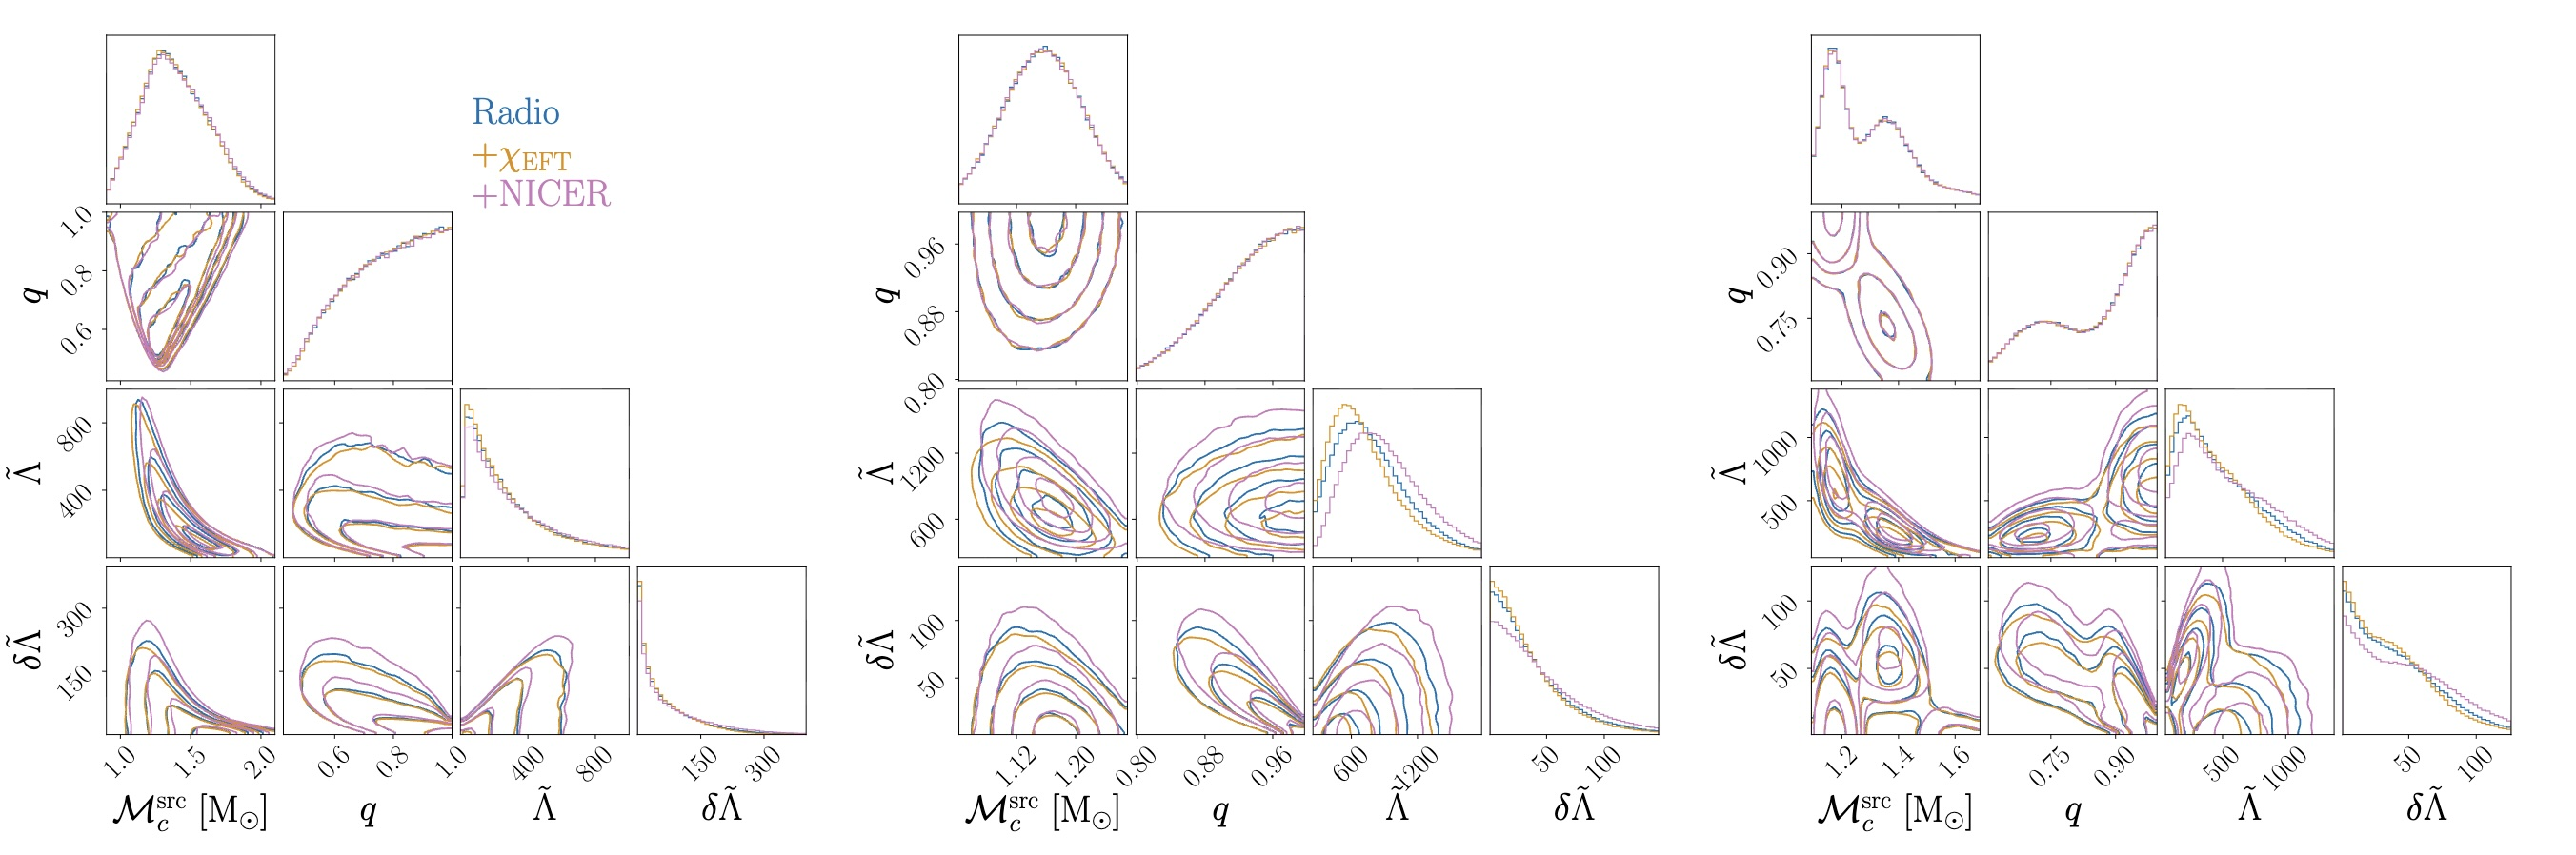
\includegraphics[width=0.99\linewidth]{Figures/neural_priors.jpg}
  \end{figure}
\end{frame}

\begin{frame}{Application}

  \begin{itemize}
    \item Implemented in \textsc{bilby}

    \item Consider three ``low-mass'' GWs
  

  \begin{columns}
      \begin{column}{0.30\textwidth}
        \begin{itemize}
          \item GW170817
          \item GW190425
          \item GW230529
        \end{itemize}
      \end{column}
      
      \begin{column}{0.69\textwidth}
        \begin{figure}
          \centering
          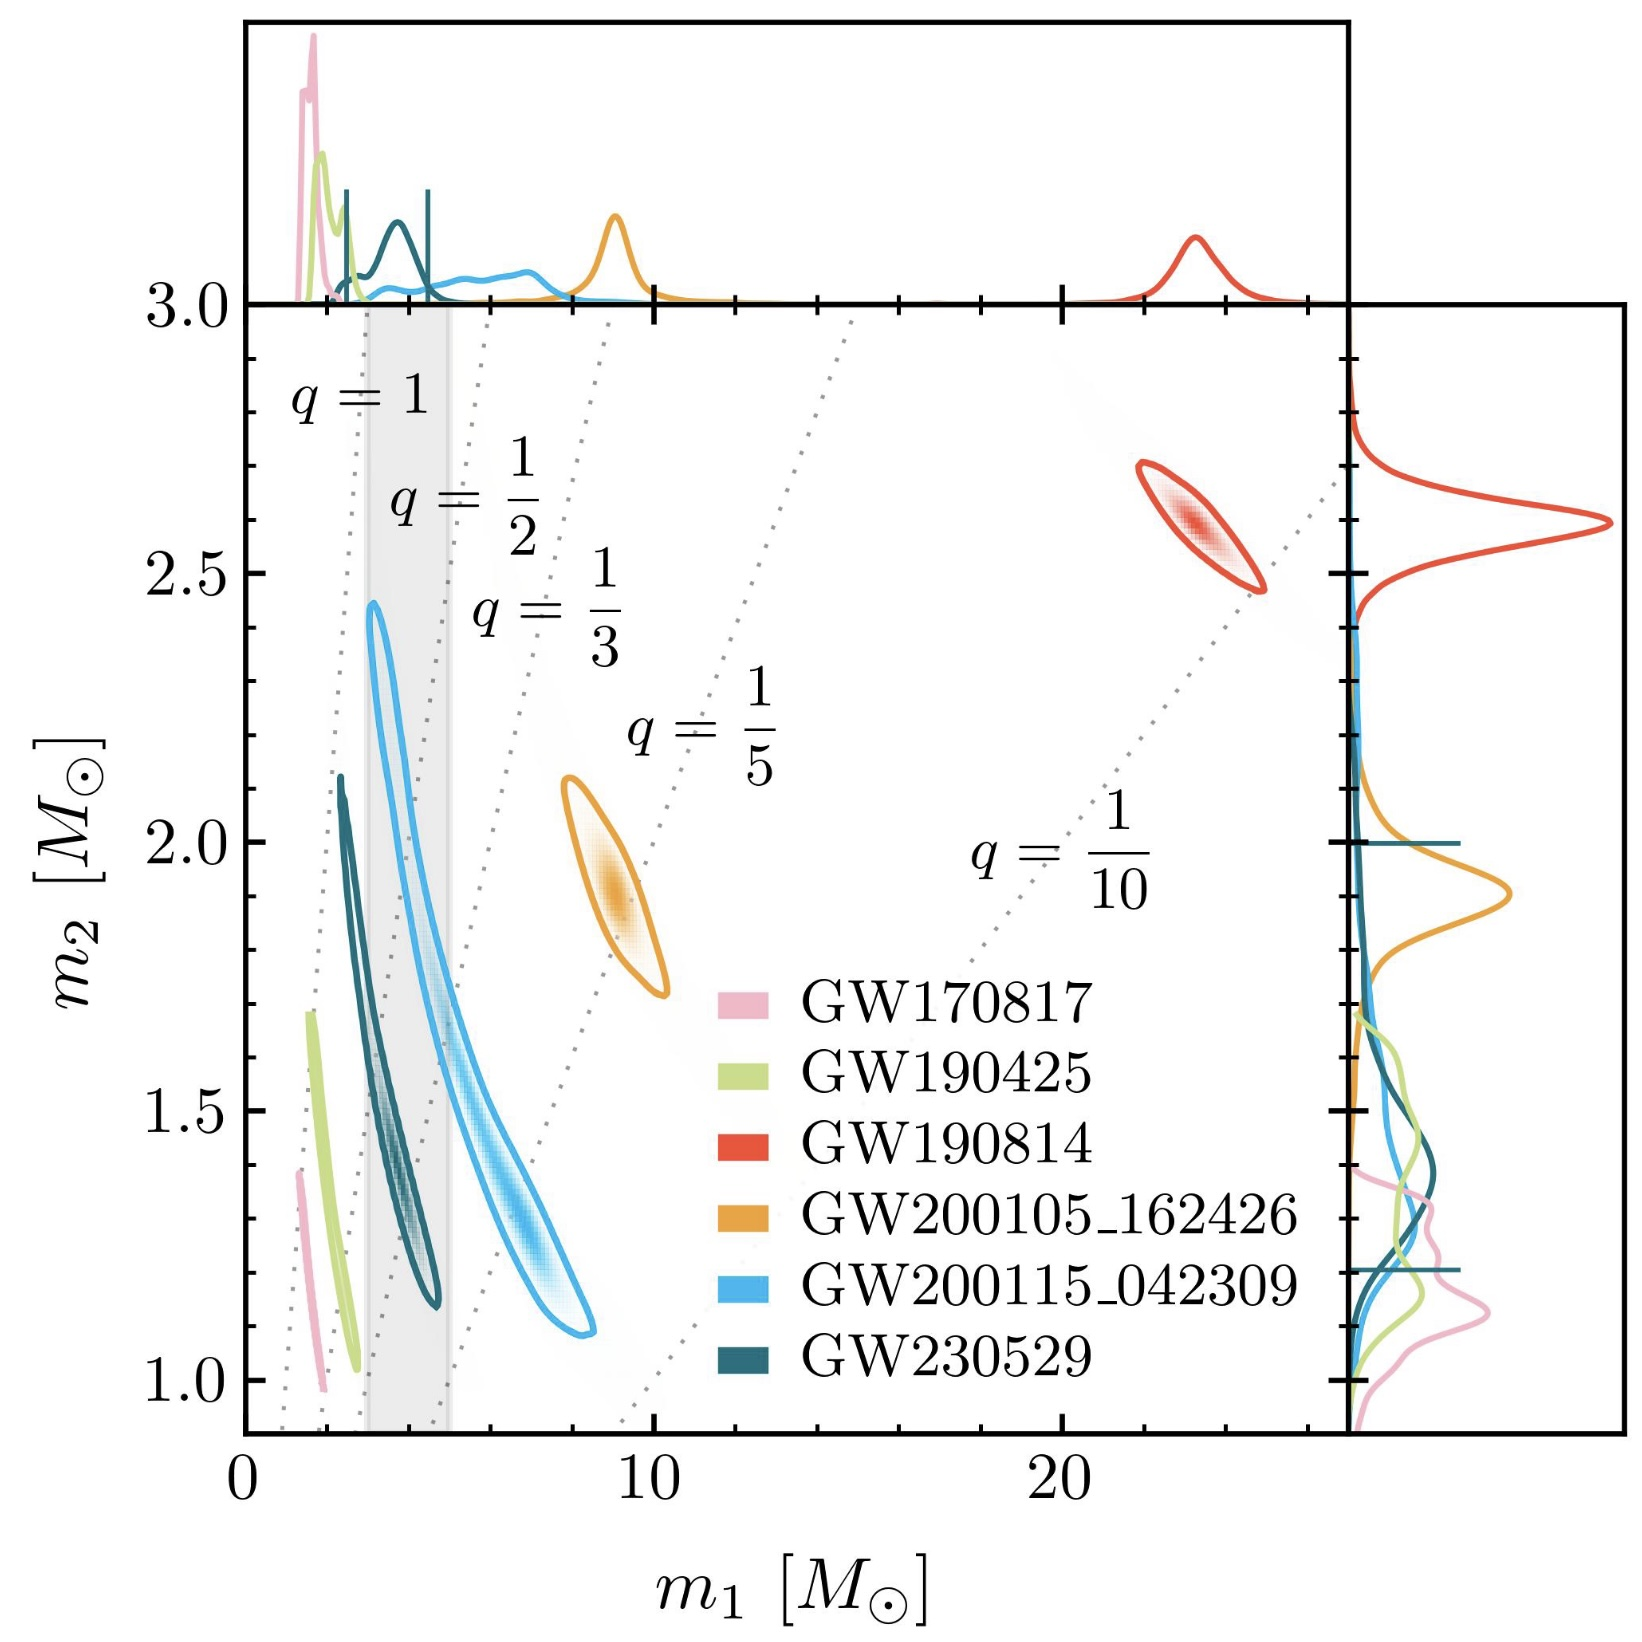
\includegraphics[width=0.75\linewidth]{Figures/GW230529_mass_diagram.jpg}
        \end{figure}
      \end{column}
    \end{columns}
    \end{itemize}

\end{frame}

\begin{frame}{GW170817 -- classification}

  Showing $\log_{10}$ Bayes factors: negative = less preferred

  \begin{itemize}
    \item Strongly prefer BNS over NSBH
    \item Gaussian population, EOS inconclusive
  \end{itemize}
  \begin{figure}
    \centering
    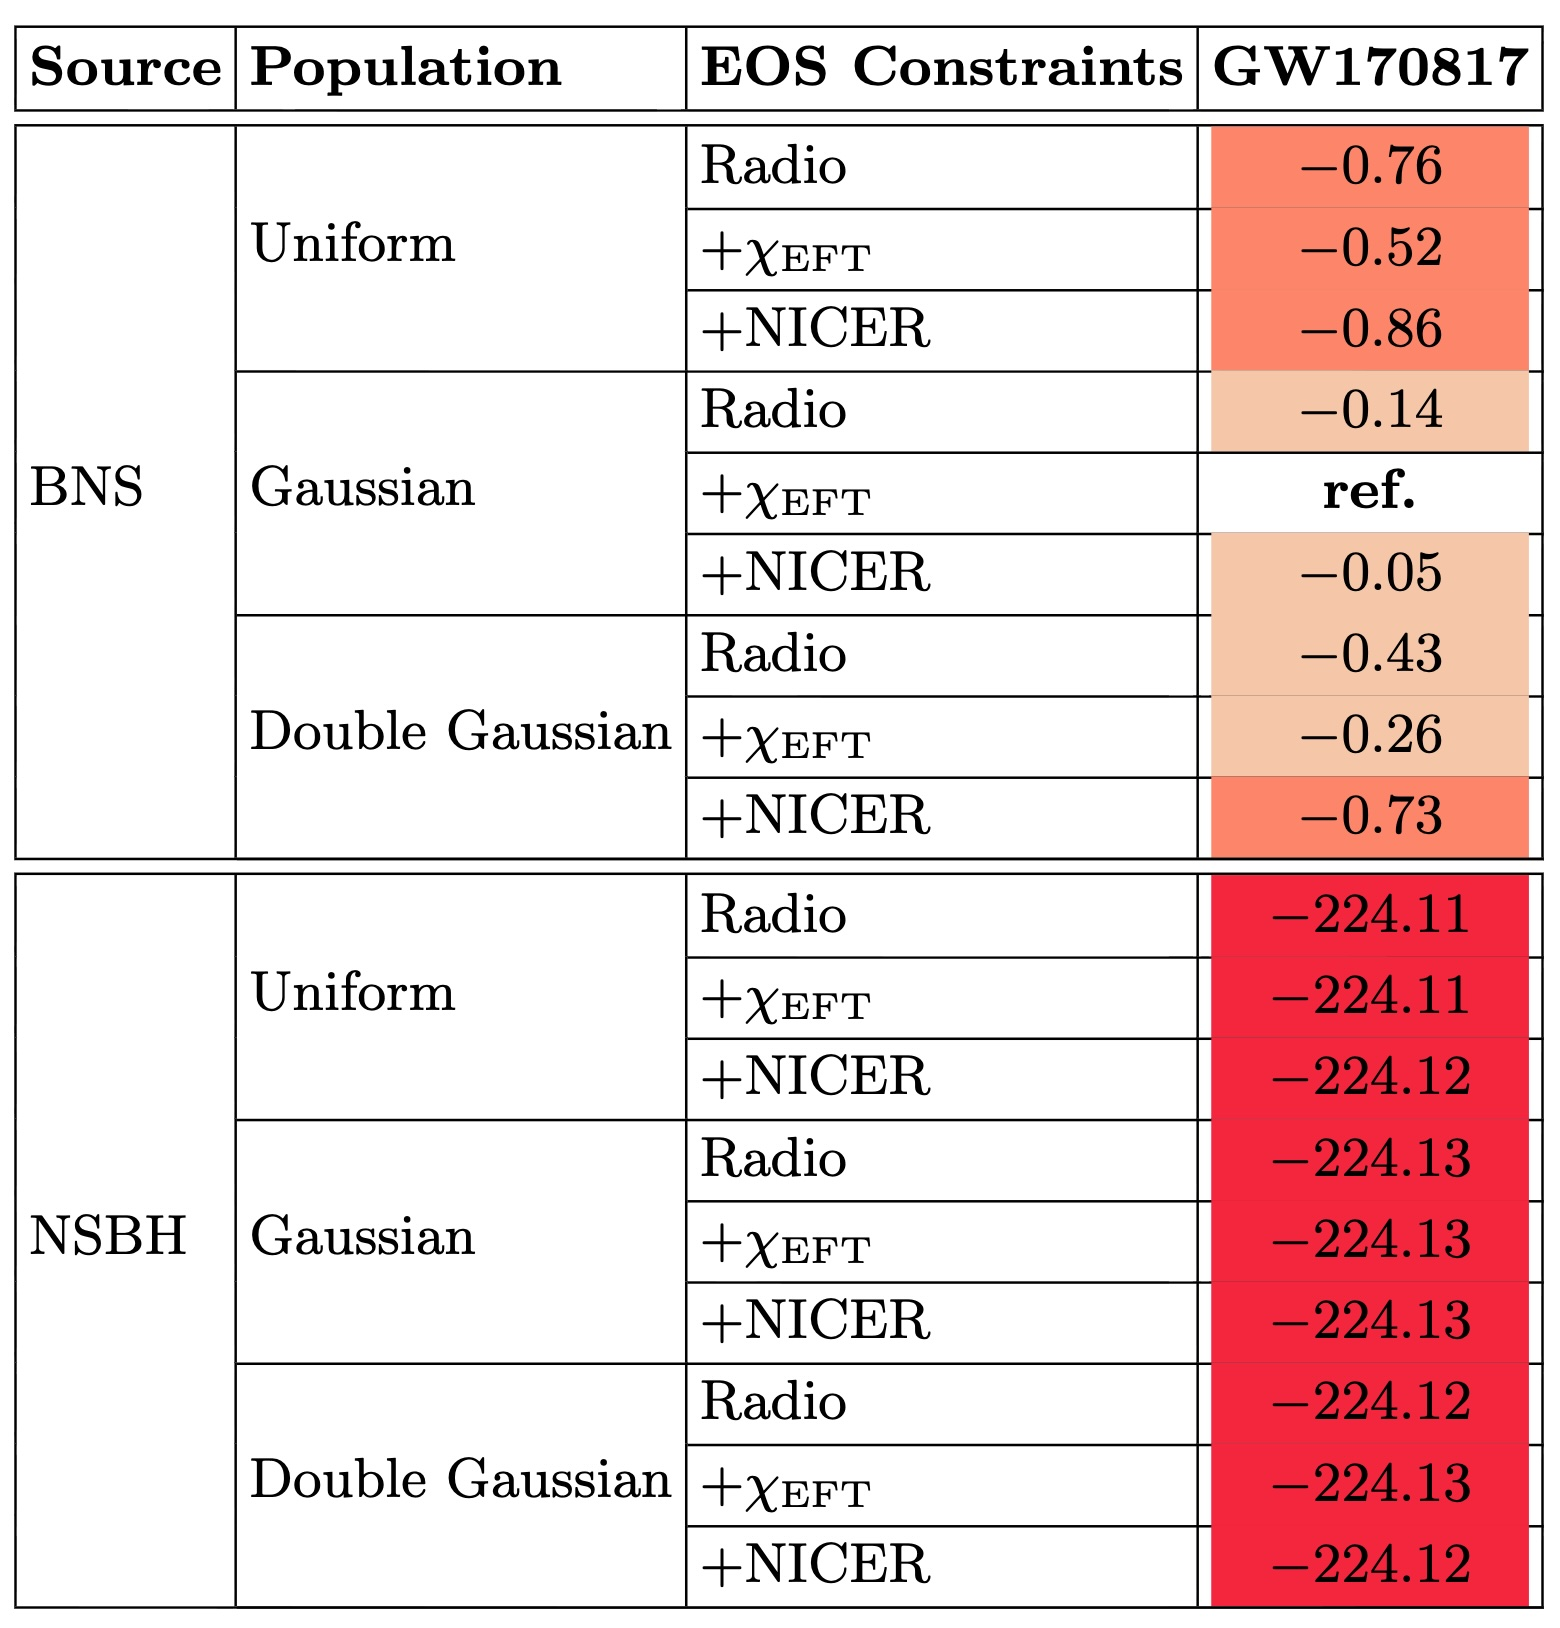
\includegraphics[width=0.50\linewidth]{Figures/GW170817_EOS_source_classification.jpg}
  \end{figure}
  
\end{frame}

\begin{frame}{GW170817 -- parameter constraints}

  \begin{itemize}
    \item More equal mass ratio $q\geq 0.9$
    \item $\tilde{\Lambda}$ bimodal, resolved by extra EOS information
  \end{itemize}

  \begin{figure}
    \centering
    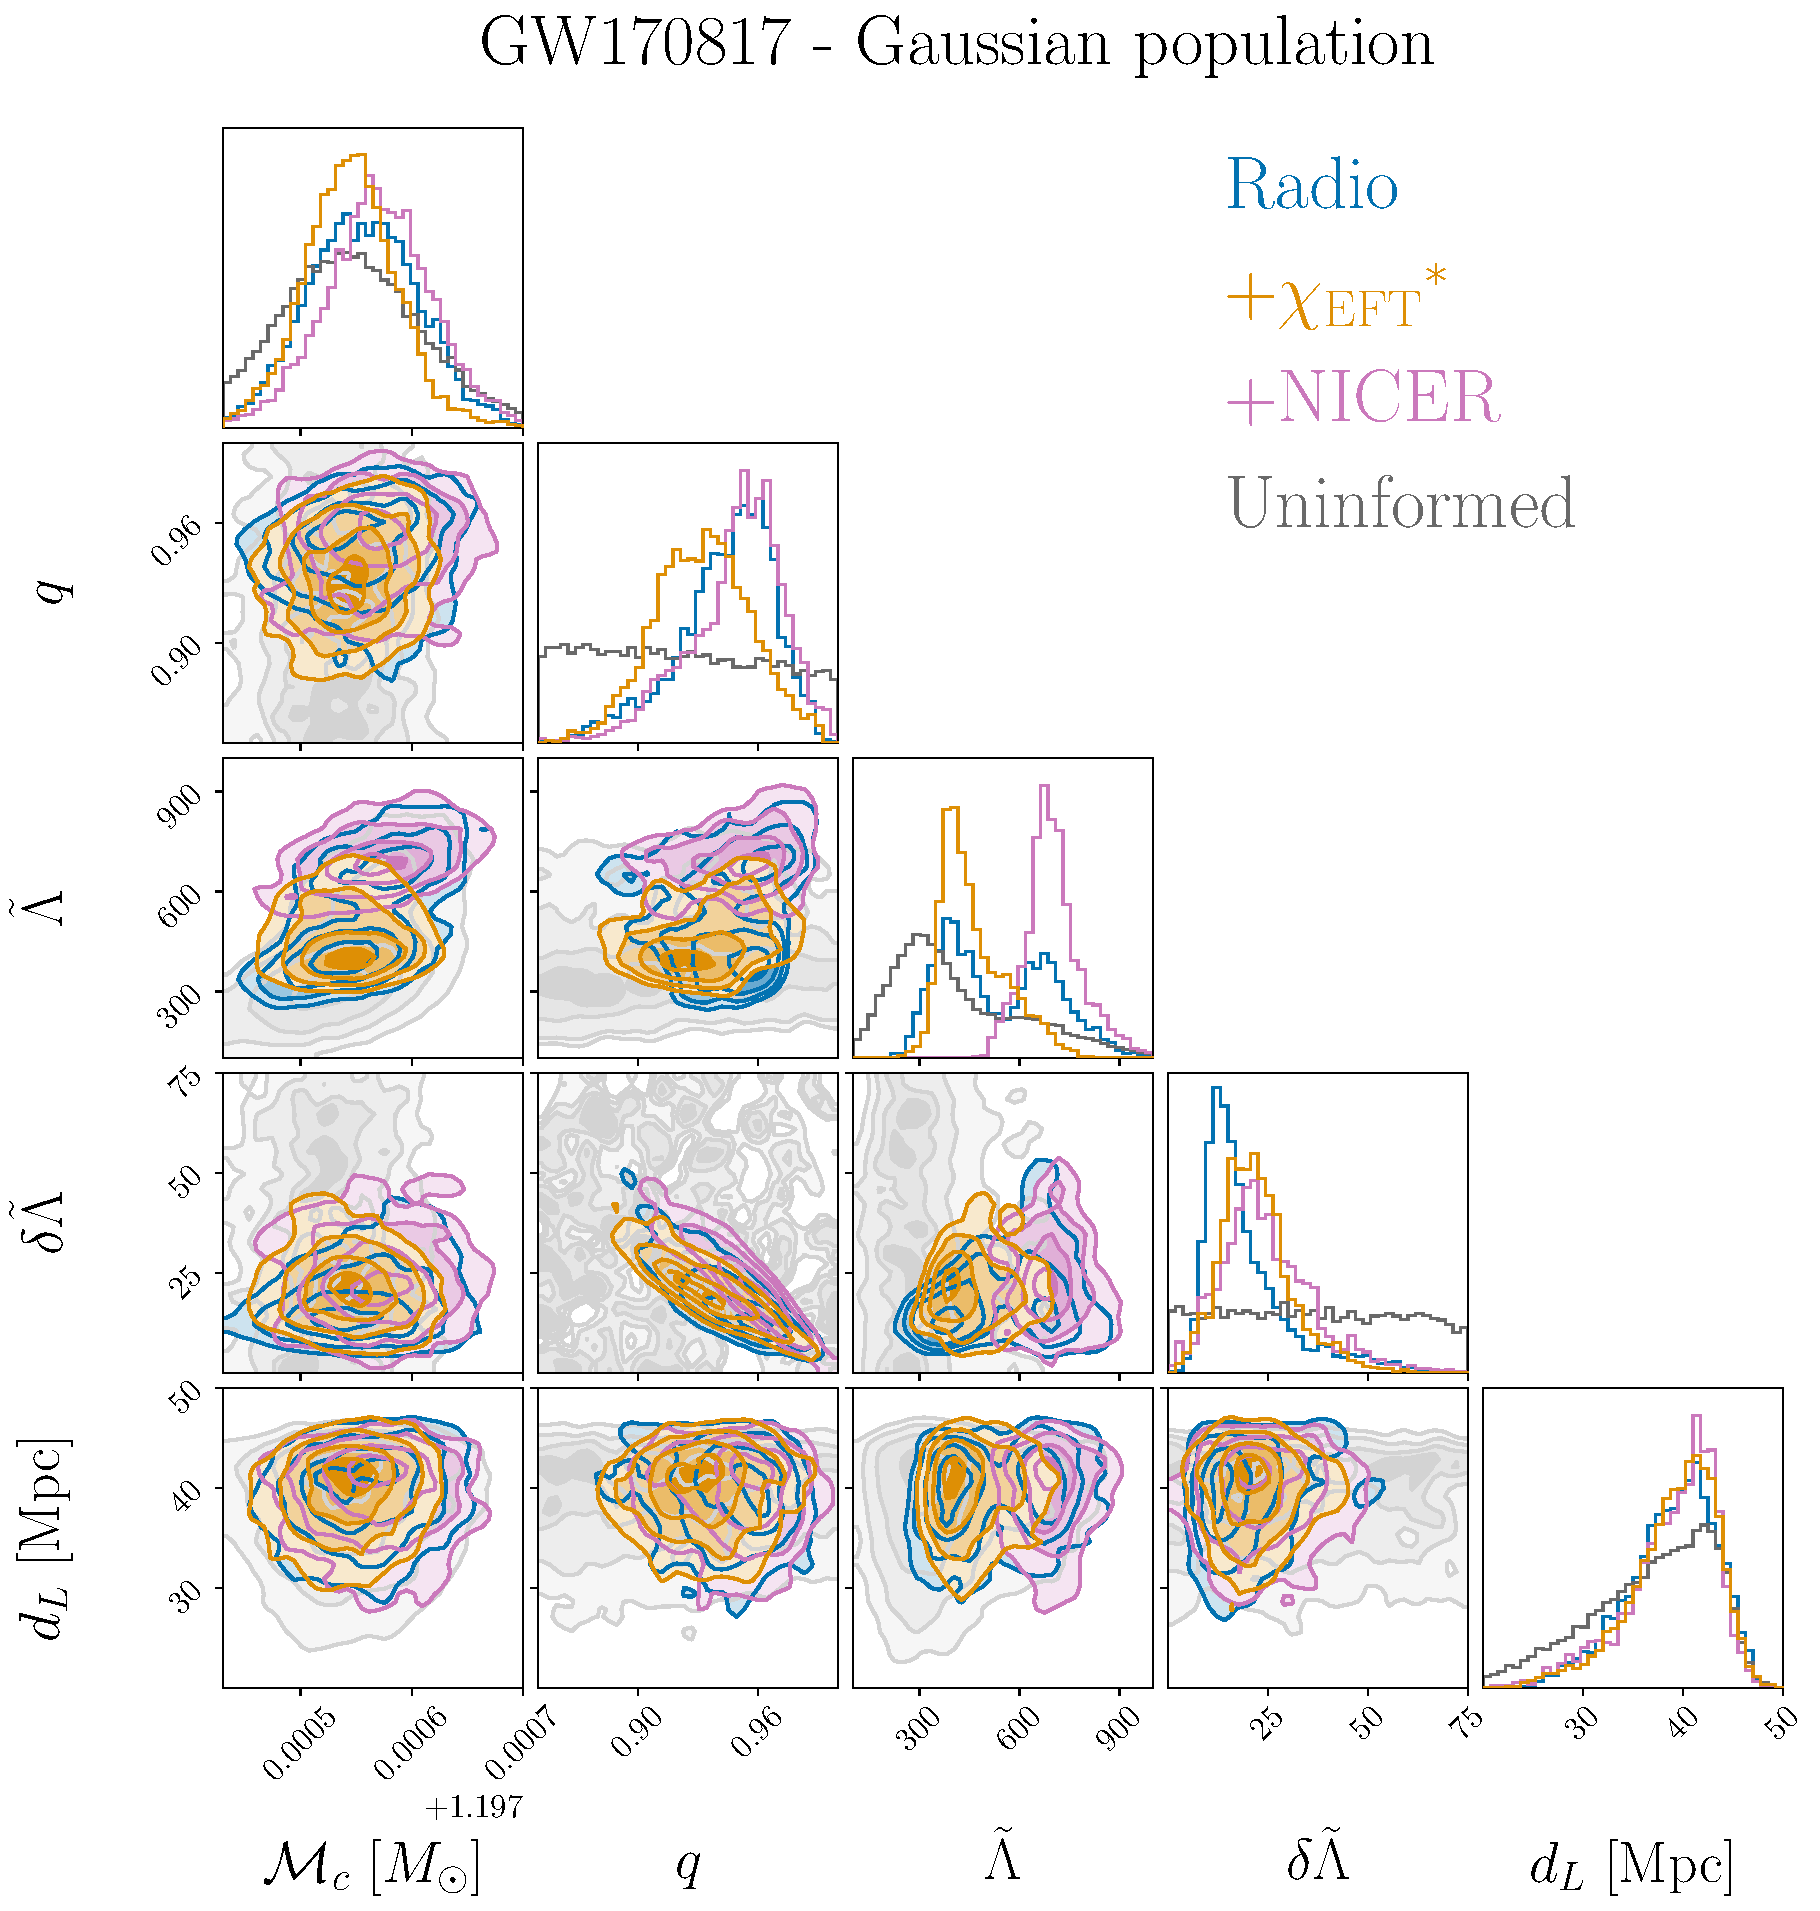
\includegraphics[width=0.525\linewidth]{Figures/GW170817_corner_gaussian_bns_PRESENTATION.pdf}
  \end{figure}
\end{frame}


\begin{frame}{GW190425 -- classification}

  Showing $\log_{10}$ Bayes factors: negative = less preferred
  \begin{itemize}
    \item Prefer BNS over NSBH, but less conclusive
    \item Most consistent with uniform population
  \end{itemize}

  \begin{figure}
    \centering
    \includegraphics[width=0.50\linewidth]{Figures/GW190425_EOS_source_classification.jpg}
  \end{figure}
\end{frame}

\begin{frame}{GW190425 -- parameter constraints}

  \begin{itemize}
    \item Less equal masses ($q\leq 0.9$)
    \item Higher distances
  \end{itemize}

  \begin{figure}
    \centering
    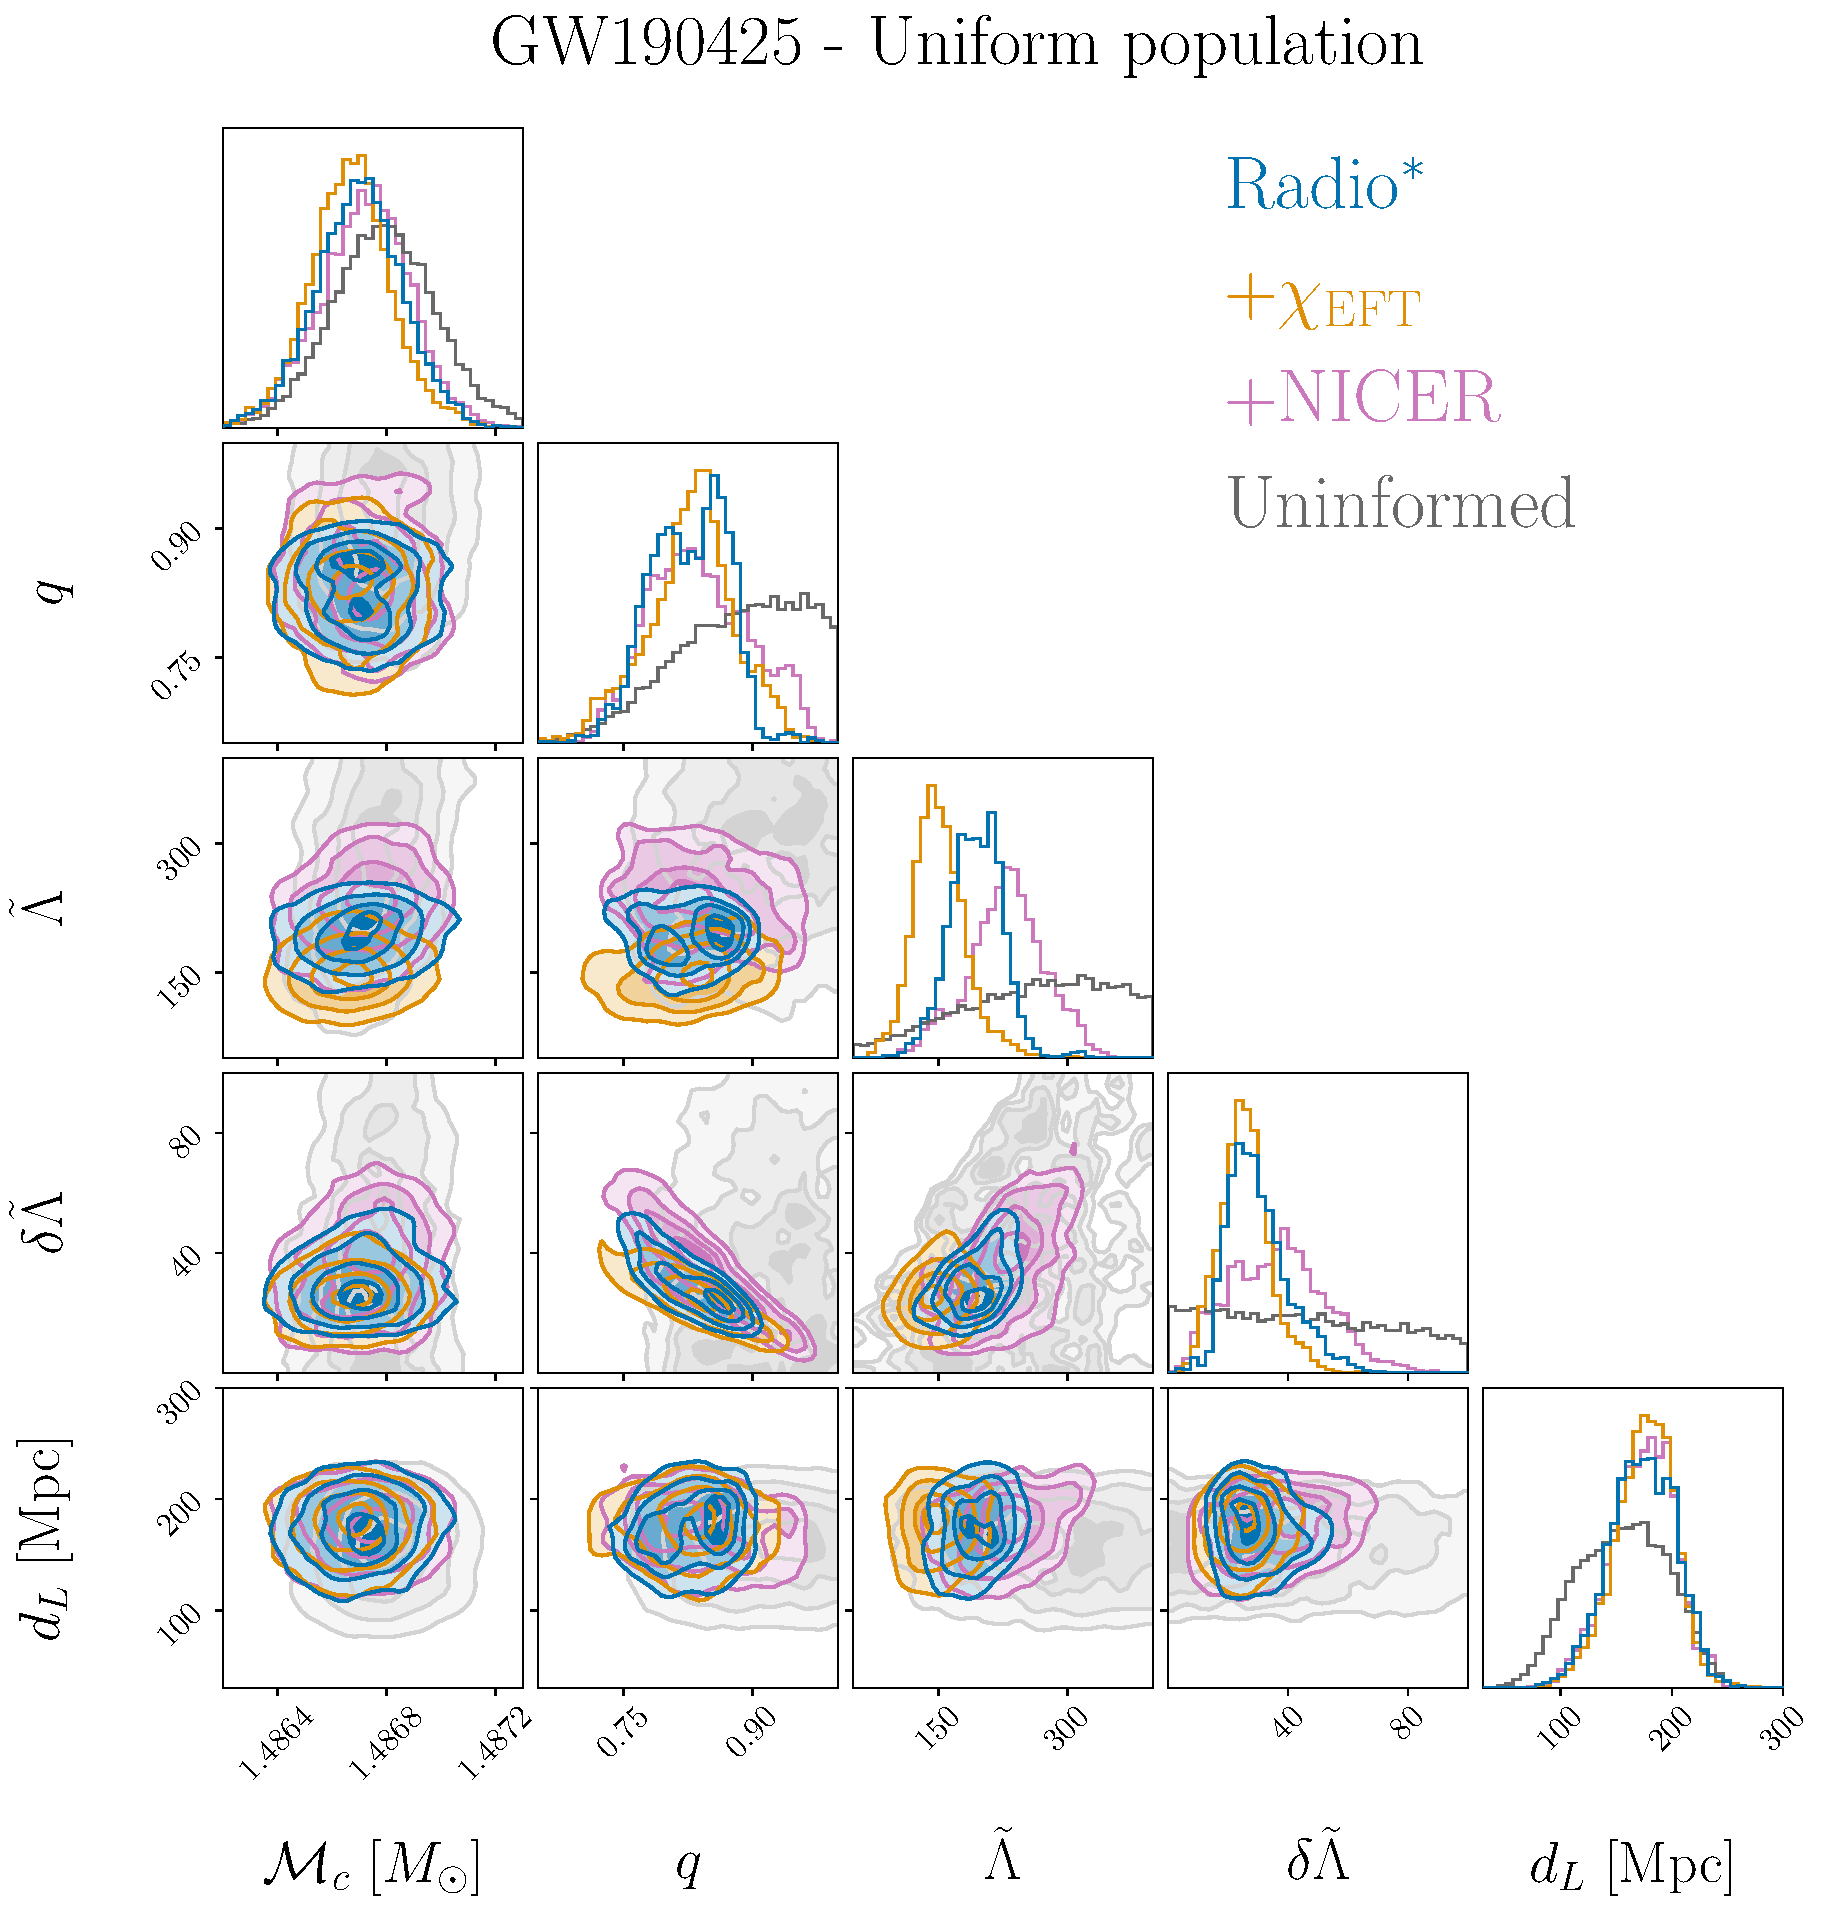
\includegraphics[width=0.525\linewidth]{Figures/GW190425_corner_uniform_bns_PRESENTATION.pdf}
  \end{figure}
\end{frame}

\begin{frame}{GW230529 -- classification}

  Showing $\log_{10}$ Bayes factors: negative = less preferred
  \begin{itemize}
    \item Decisive evidence for NSBH over BNS
    \item Weak evidence for population or EOS (low SNR)
  \end{itemize}

  \begin{figure}
    \centering
    \includegraphics[width=0.50\linewidth]{Figures/GW230529_EOS_source_classification.jpg}
  \end{figure}
\end{frame}


\begin{frame}{GW230529 -- parameter constraints}

  \begin{itemize}
    \item Mass ratio more constrained $\rightarrow$ $\chi_{1z}$ more constrained
    \item Higher distances
  \end{itemize}

  \begin{figure}
    \centering
    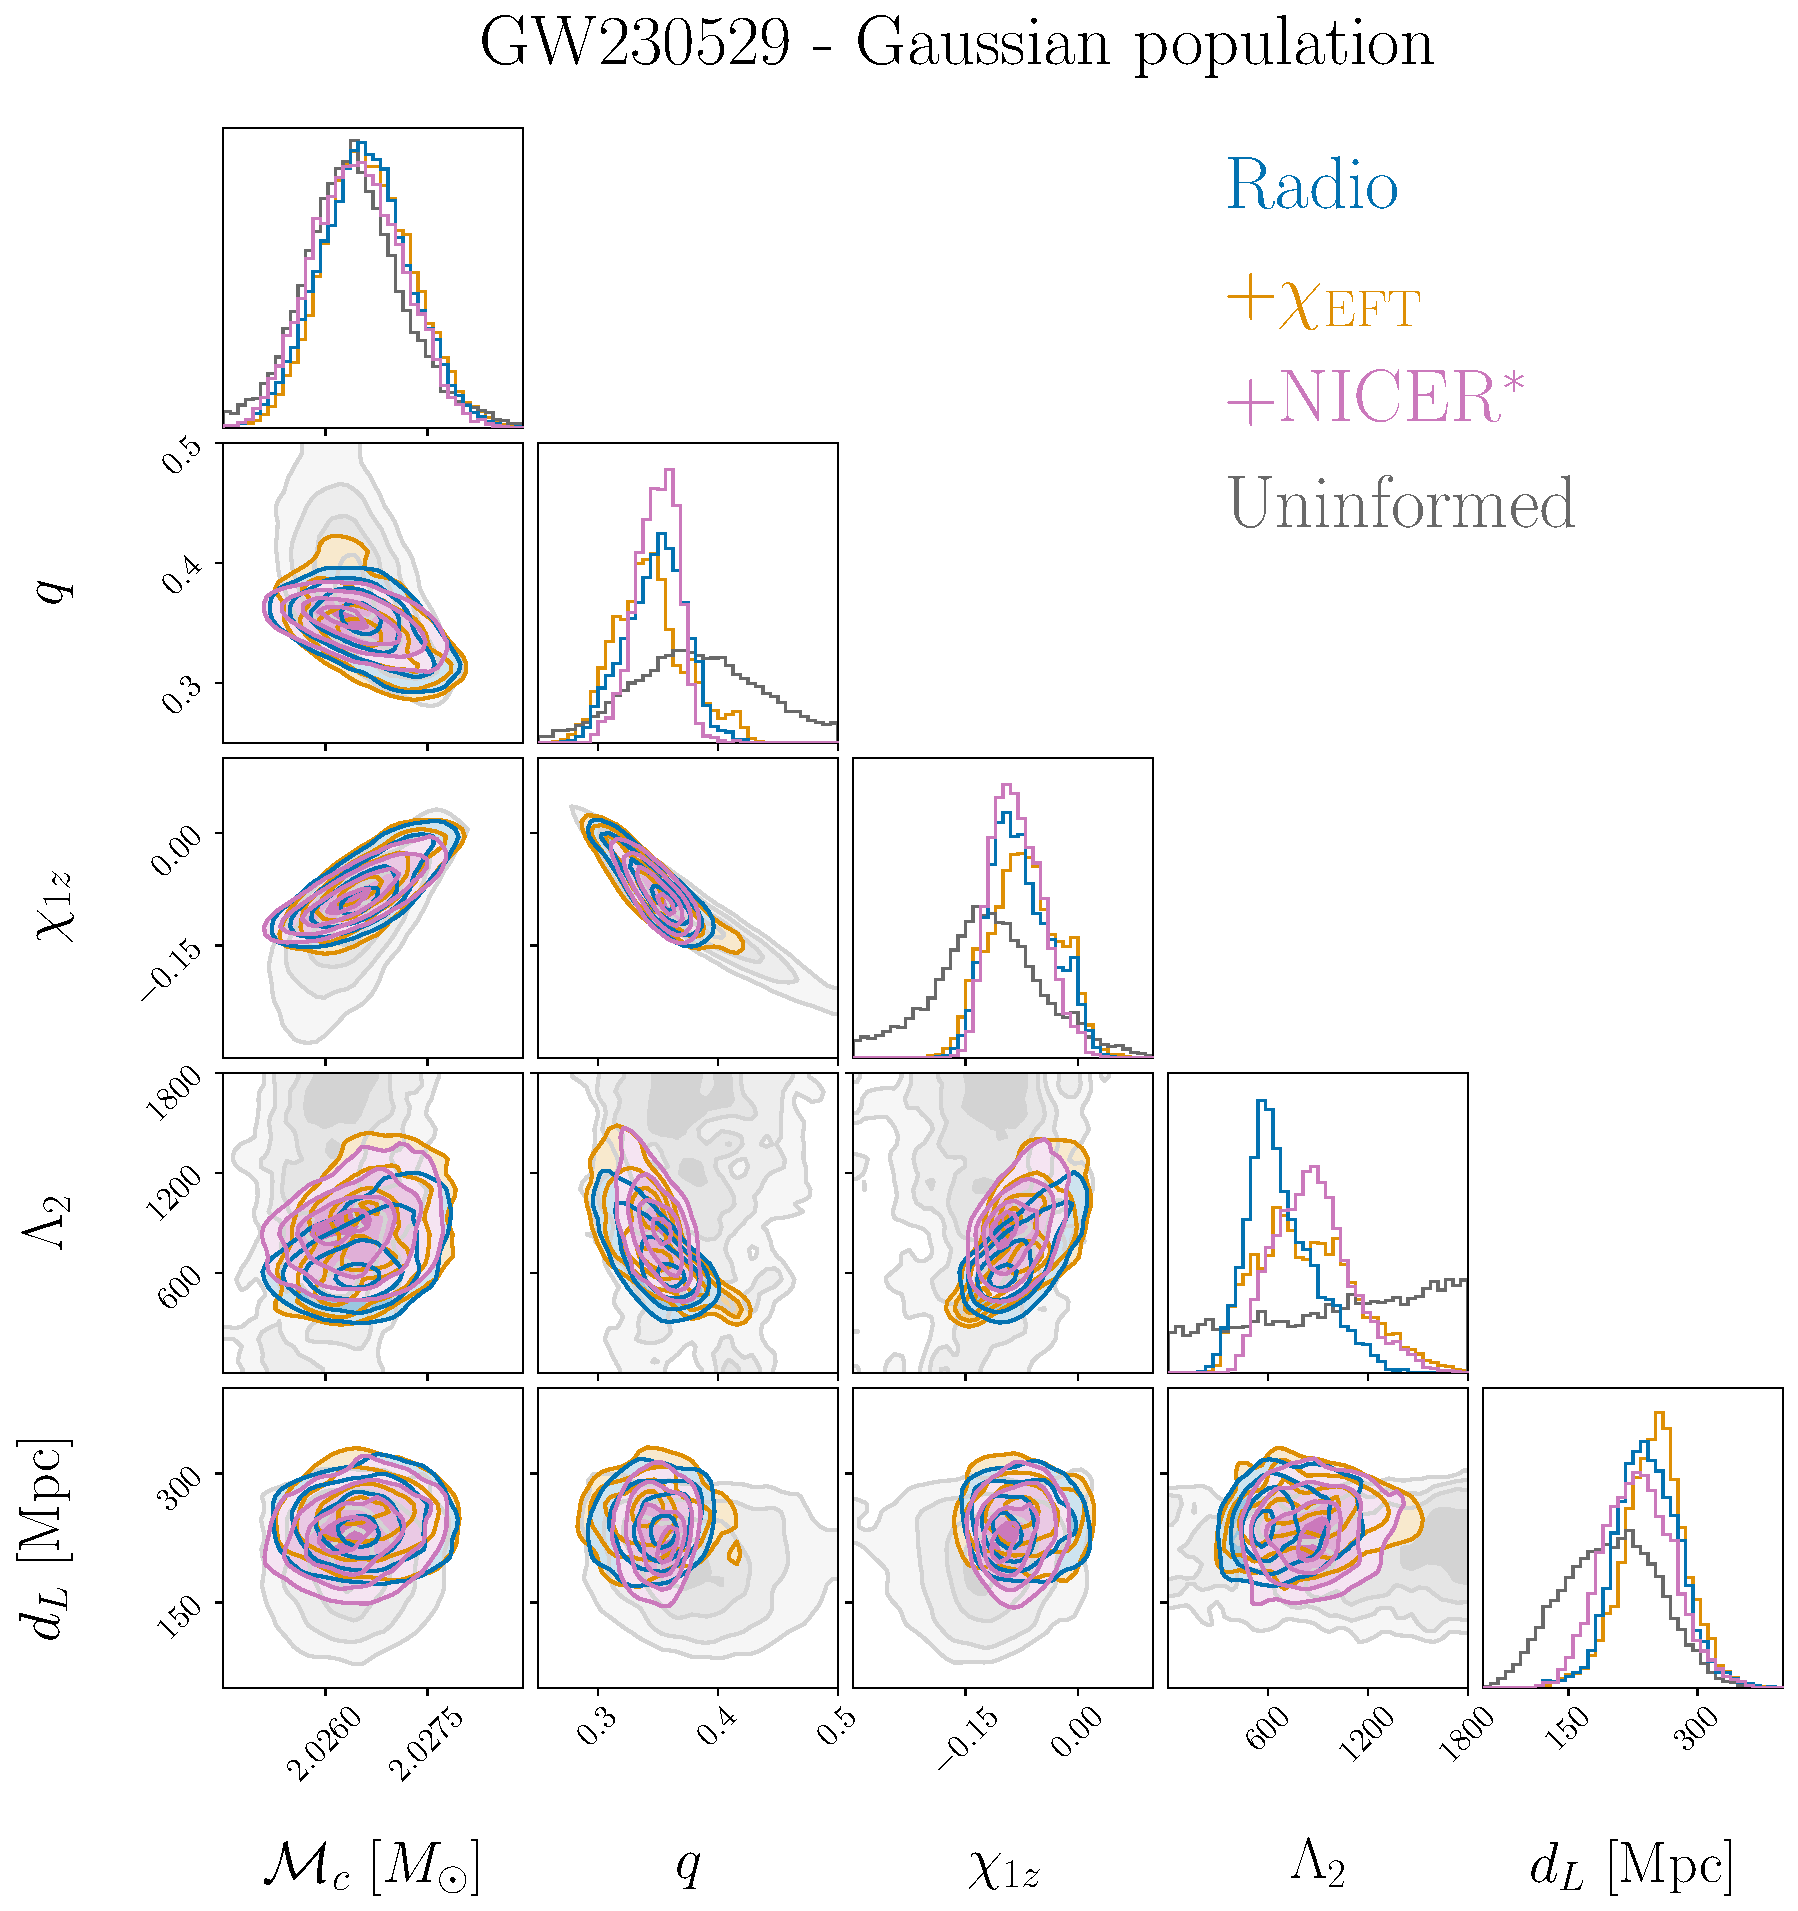
\includegraphics[width=0.525\linewidth]{Figures/GW230529_corner_gaussian_nsbh_PRESENTATION.pdf}
  \end{figure}
\end{frame}



\section{Conclusion}

\begin{frame}{Conclusion}
  \def\x{4mm}
  \def\y{1mm}

  \begin{itemize}
    \item Progress on scalable Bayesian inference, with minimal comrpomises
 
    \vspace{\x}

    \item Accelerate likelihood-based inference with
    \begin{itemize}
      \vspace{\y}
      \item \textsc{JAX}: GPU for faster likelihoods

      \vspace{\y}

      \item Normalizing flows to aid in inference (sampling, priors)
    \end{itemize}

    \vspace{\x}

    \item GWs: checked for LVK, work in progress for ET: waveform experts needed!

    \vspace{\x}

    \item Kilonova/GRB: emulators for fast inference

    \vspace{\x}

    \item EOS: scalable inference, open up systematics studies
  \end{itemize}
  
  \vspace{8mm}

  \textbf{Let's talk!}
\end{frame}

{
\usebackgroundtemplate{\transparent{0.5}{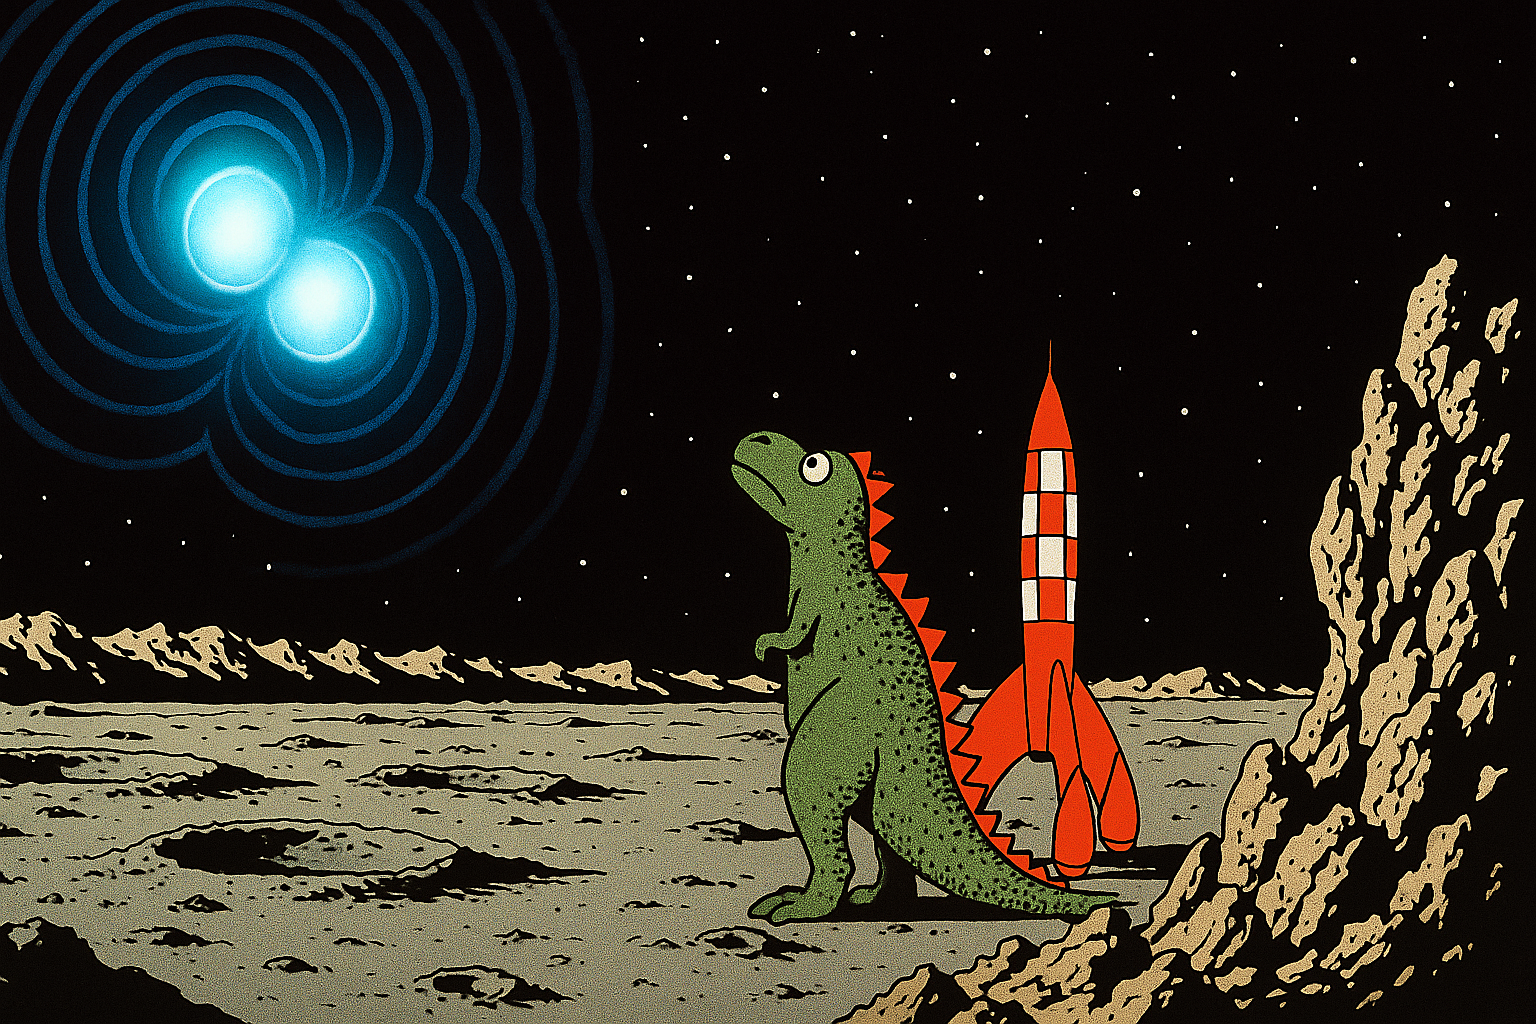
\includegraphics[width=\paperwidth,height=\paperheight]{Figures/tintin_dinosaur.png}}}

\begin{frame}[plain, noframenumbering]

  \begin{tikzpicture}[remember picture,overlay]
    \node[fill=customblue, fill opacity=0.75, text opacity=1, rounded corners=10pt, inner sep=15pt] at ([yshift=2cm]current page.center) {
      \begin{minipage}{0.8\textwidth}
        \centering
        \textbf{Thanks for listening!}
      \end{minipage}
    };
  \end{tikzpicture}

  \end{frame}
}

% \begin{frame}[plain, noframenumbering]{Thank you for your attention!}

%   \def\x{0.5mm}
  
%   Software written in \textsc{jax}~\ghlink{jax-ml/jax}:
%   \begin{itemize}
%     \vspace{\x}
%     \item \textsc{flowMC} \ghlink{kazewong/flowMC}~\cite{Gabrie:2021tlu, Wong:2022xvh}

%     \vspace{\x}

%     \item \textsc{Jim} \ghlink{kazewong/jim}~\cite{Wong:2023lgb,Wouters:2024oxj} \enumicon{1} \enumicon{2} \enumicon{4}

%     \vspace{\x}

%     \item \textsc{fiesta} \ghlink{ThibeauWouters/fiestaEM} \enumicon{2} %(work in progress...)

%     \vspace{\x}

%     \item \textsc{Jester} \ghlink{nuclear-multimessenger-astronomy/jester}~\cite{Wouters:2025zju} (built with \textsc{diffrax}~\ghlink{patrick-kidger/diffrax}) \enumicon{3}

%     \vspace{\x}

%     \item \textsc{harmonic} \ghlink{astro-informatics/harmonic}~\cite{mcewen2023machinelearningassistedbayesian, polanska2024learnedharmonicmeanestimation, Polanska:2024zpn}
%   \end{itemize}

%   \centering
%   \incfig[0.975\textwidth]{talk_overview}
% \end{frame}

\begin{frame}[allowframebreaks]{References}
  \nocite{my_misc_entry}
  \nocite{Kuifje}
  \printbibliography
\end{frame}

\appendix 


\begin{frame}[allowframebreaks]{Evidence calculation: \textsc{harmonic}}

  Evidence $Z$ can be computed from posterior samples with \textsc{harmonic}~\cite{mcewen2023machinelearningassistedbayesian} with the \red{harmonic mean estimator}

  \begin{align*}
    \rho &\equiv \mathbb{E}_{P(\theta|d)}\left[\frac{1}{L(\theta)}\right] \\ 
    &= \int \diff \theta \frac{1}{\mathcal{L}(\theta)} P(\theta | d) \\
    &= \int \diff \theta \frac{1}{\mathcal{L}(\theta)} \frac{\mathcal{L}(\theta) \pi(\theta)}{Z} = \frac{1}{Z}
  \end{align*}

  Therefore, estimate $\rho$ with posterior samples:
  \begin{equation*}
    \hat{\rho} = \frac1N \sum_{i=1}^N \frac{1}{\mathcal{L}(\theta)}, \quad \theta_i \sim P(\theta|d)
  \end{equation*}

  Can be interpreted as importance sampling
  \begin{equation*}
    \rho = \int \diff \theta \frac1Z \frac{\pi(\theta)}{P(\theta | d)} P(\theta | d) \, ,
  \end{equation*}
  \textbf{but} with target = prior and sampling density = posterior. Therefore, importance sampling is inefficient -- how to solve?

  New proposal:
  \begin{align*}
    \rho &= \mathbb{E}_{P(\theta| d)}\left[ \frac{\varphi(\theta)}{\mathcal{L}(\theta)\pi(\theta)} \right] \\
    &= \int \mathrm{d}\theta \, \frac{\varphi(\theta)}{\mathcal{L}(\theta)\pi(\theta)} \, P(\theta| d) \\
    &= \int \mathrm{d}\theta \, \frac{\varphi(\theta)}{\mathcal{L}(\theta)\pi(\theta)} \, \frac{\mathcal{L}(\theta)\pi(\theta)}{Z} = \frac{1}{Z}
  \end{align*}

  Use the following estimator:
  \begin{equation*}
    \hat{\rho} = \frac{1}{N} \sum_{i=1}^N \frac{\varphi(\theta_i)}{\mathcal{L}(\theta_i)\pi(\theta_i)}, \quad \theta_i \sim P(\theta|d)
  \end{equation*}

  \vspace{5mm}
  Replace the target distribution $\pi$ with $\varphi$: only requirement is that it is normalized 
  
  \vspace{5mm}
  In practice, this can be achieved with a normalizing flow~\cite{polanska2024learnedharmonicmeanestimation}. \\
  
  \vspace{5mm}
  This has been verified to give accurate evidences (similar values as nested sampling) when GW posteriors are used~\cite{Polanska:2024zpn}. 
\end{frame}

\begin{frame}{\textsc{harmonic} with \textsc{jim}~\cite{Polanska:2024zpn}}
  \begin{figure}
    \centering
    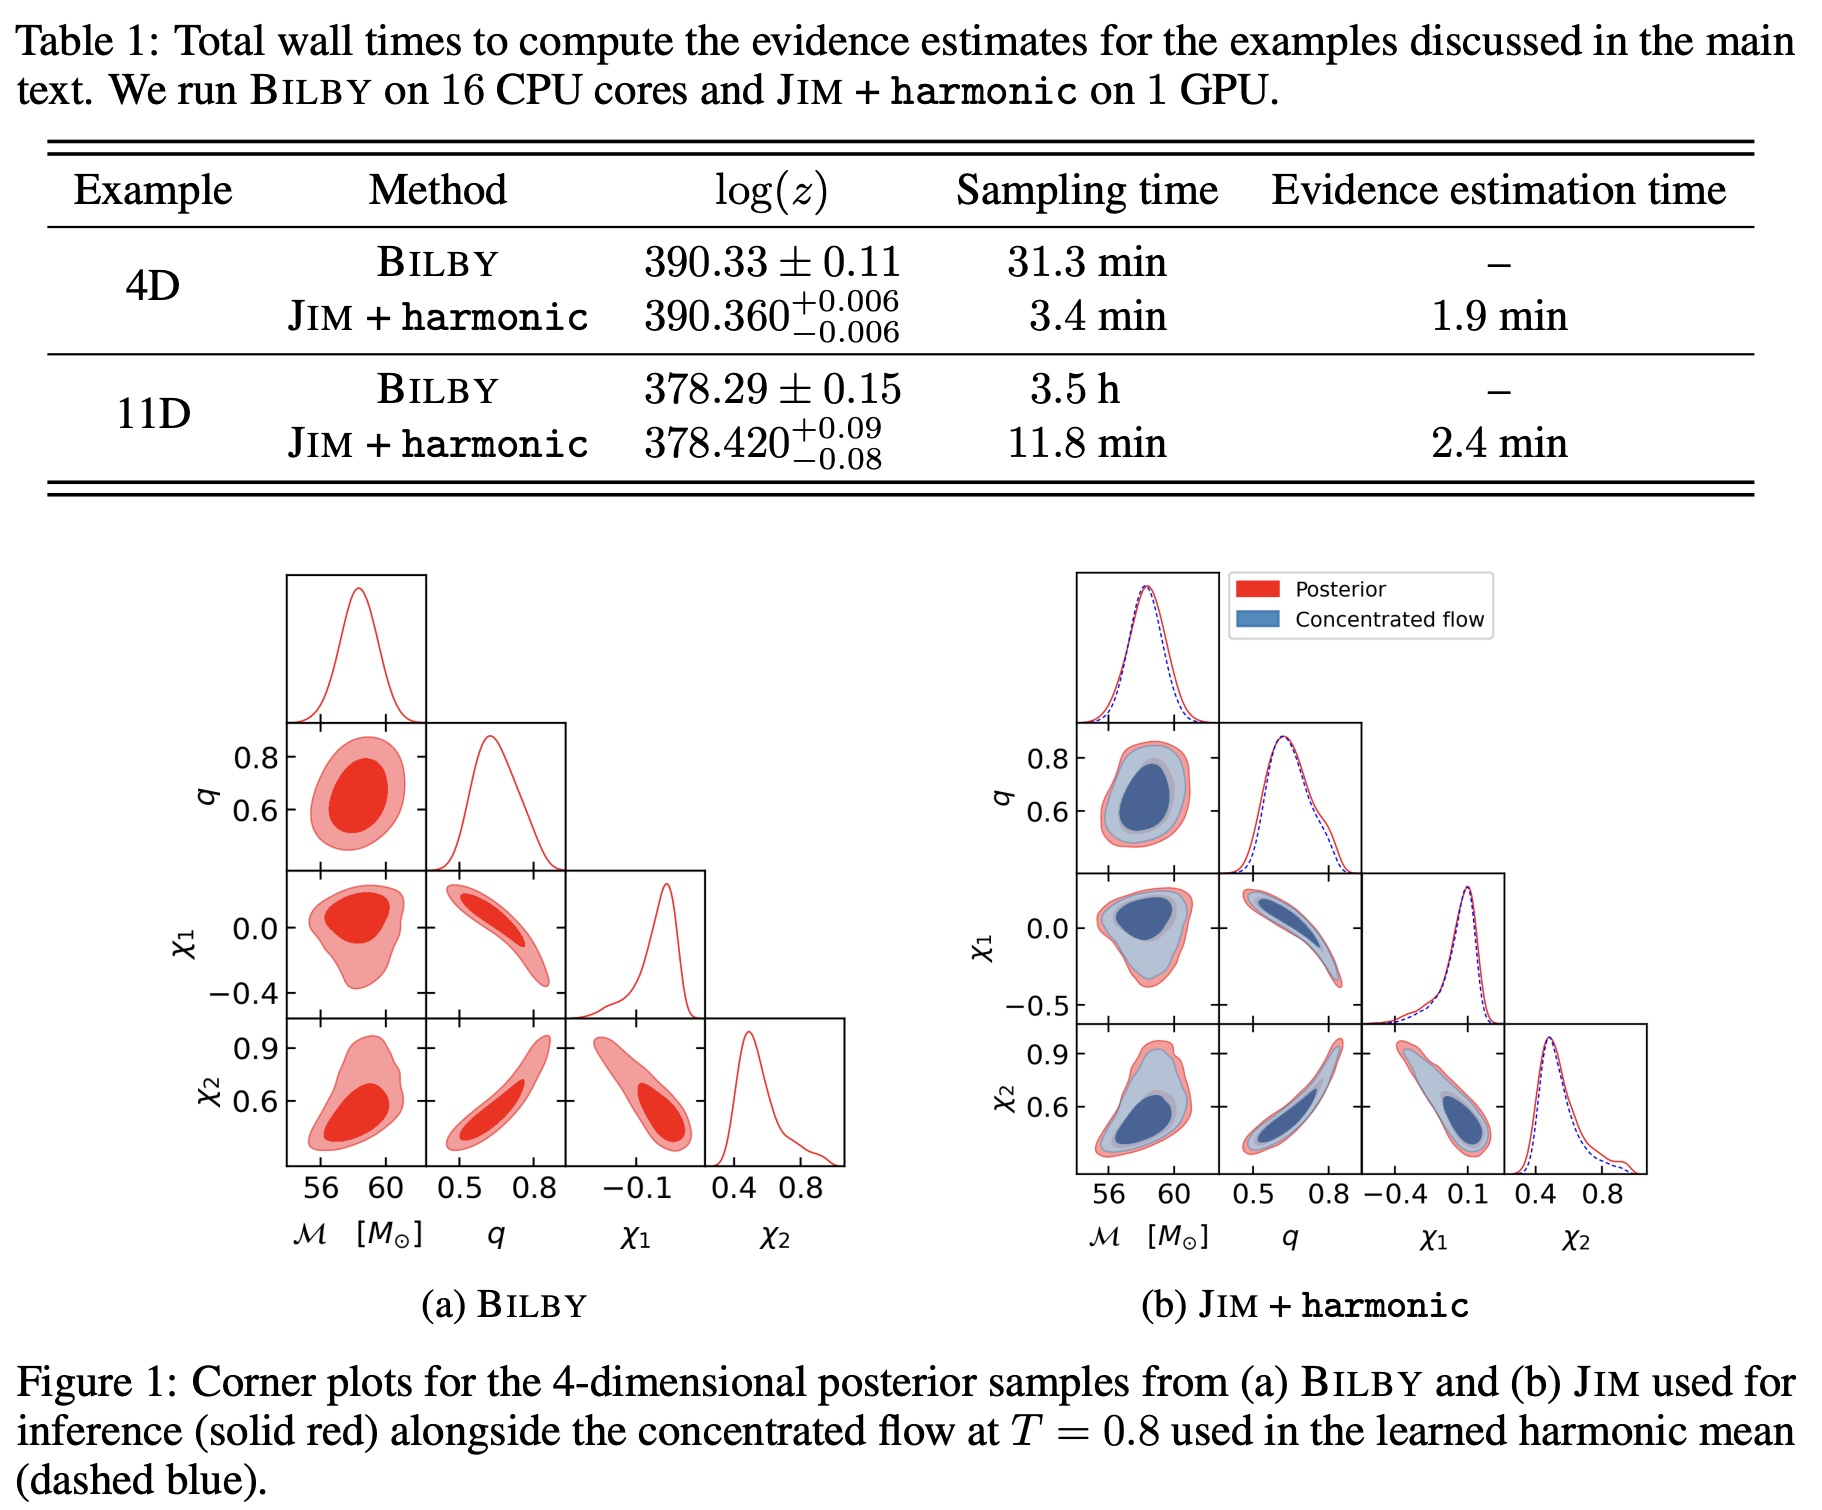
\includegraphics[scale=0.275]{Figures/polanska.jpg}
  \end{figure}
  
\end{frame}

\begin{frame}{BNS in ET-$\Delta$ example: all parameters}
  \vspace{-3mm}
  \begin{figure}
    \centering
    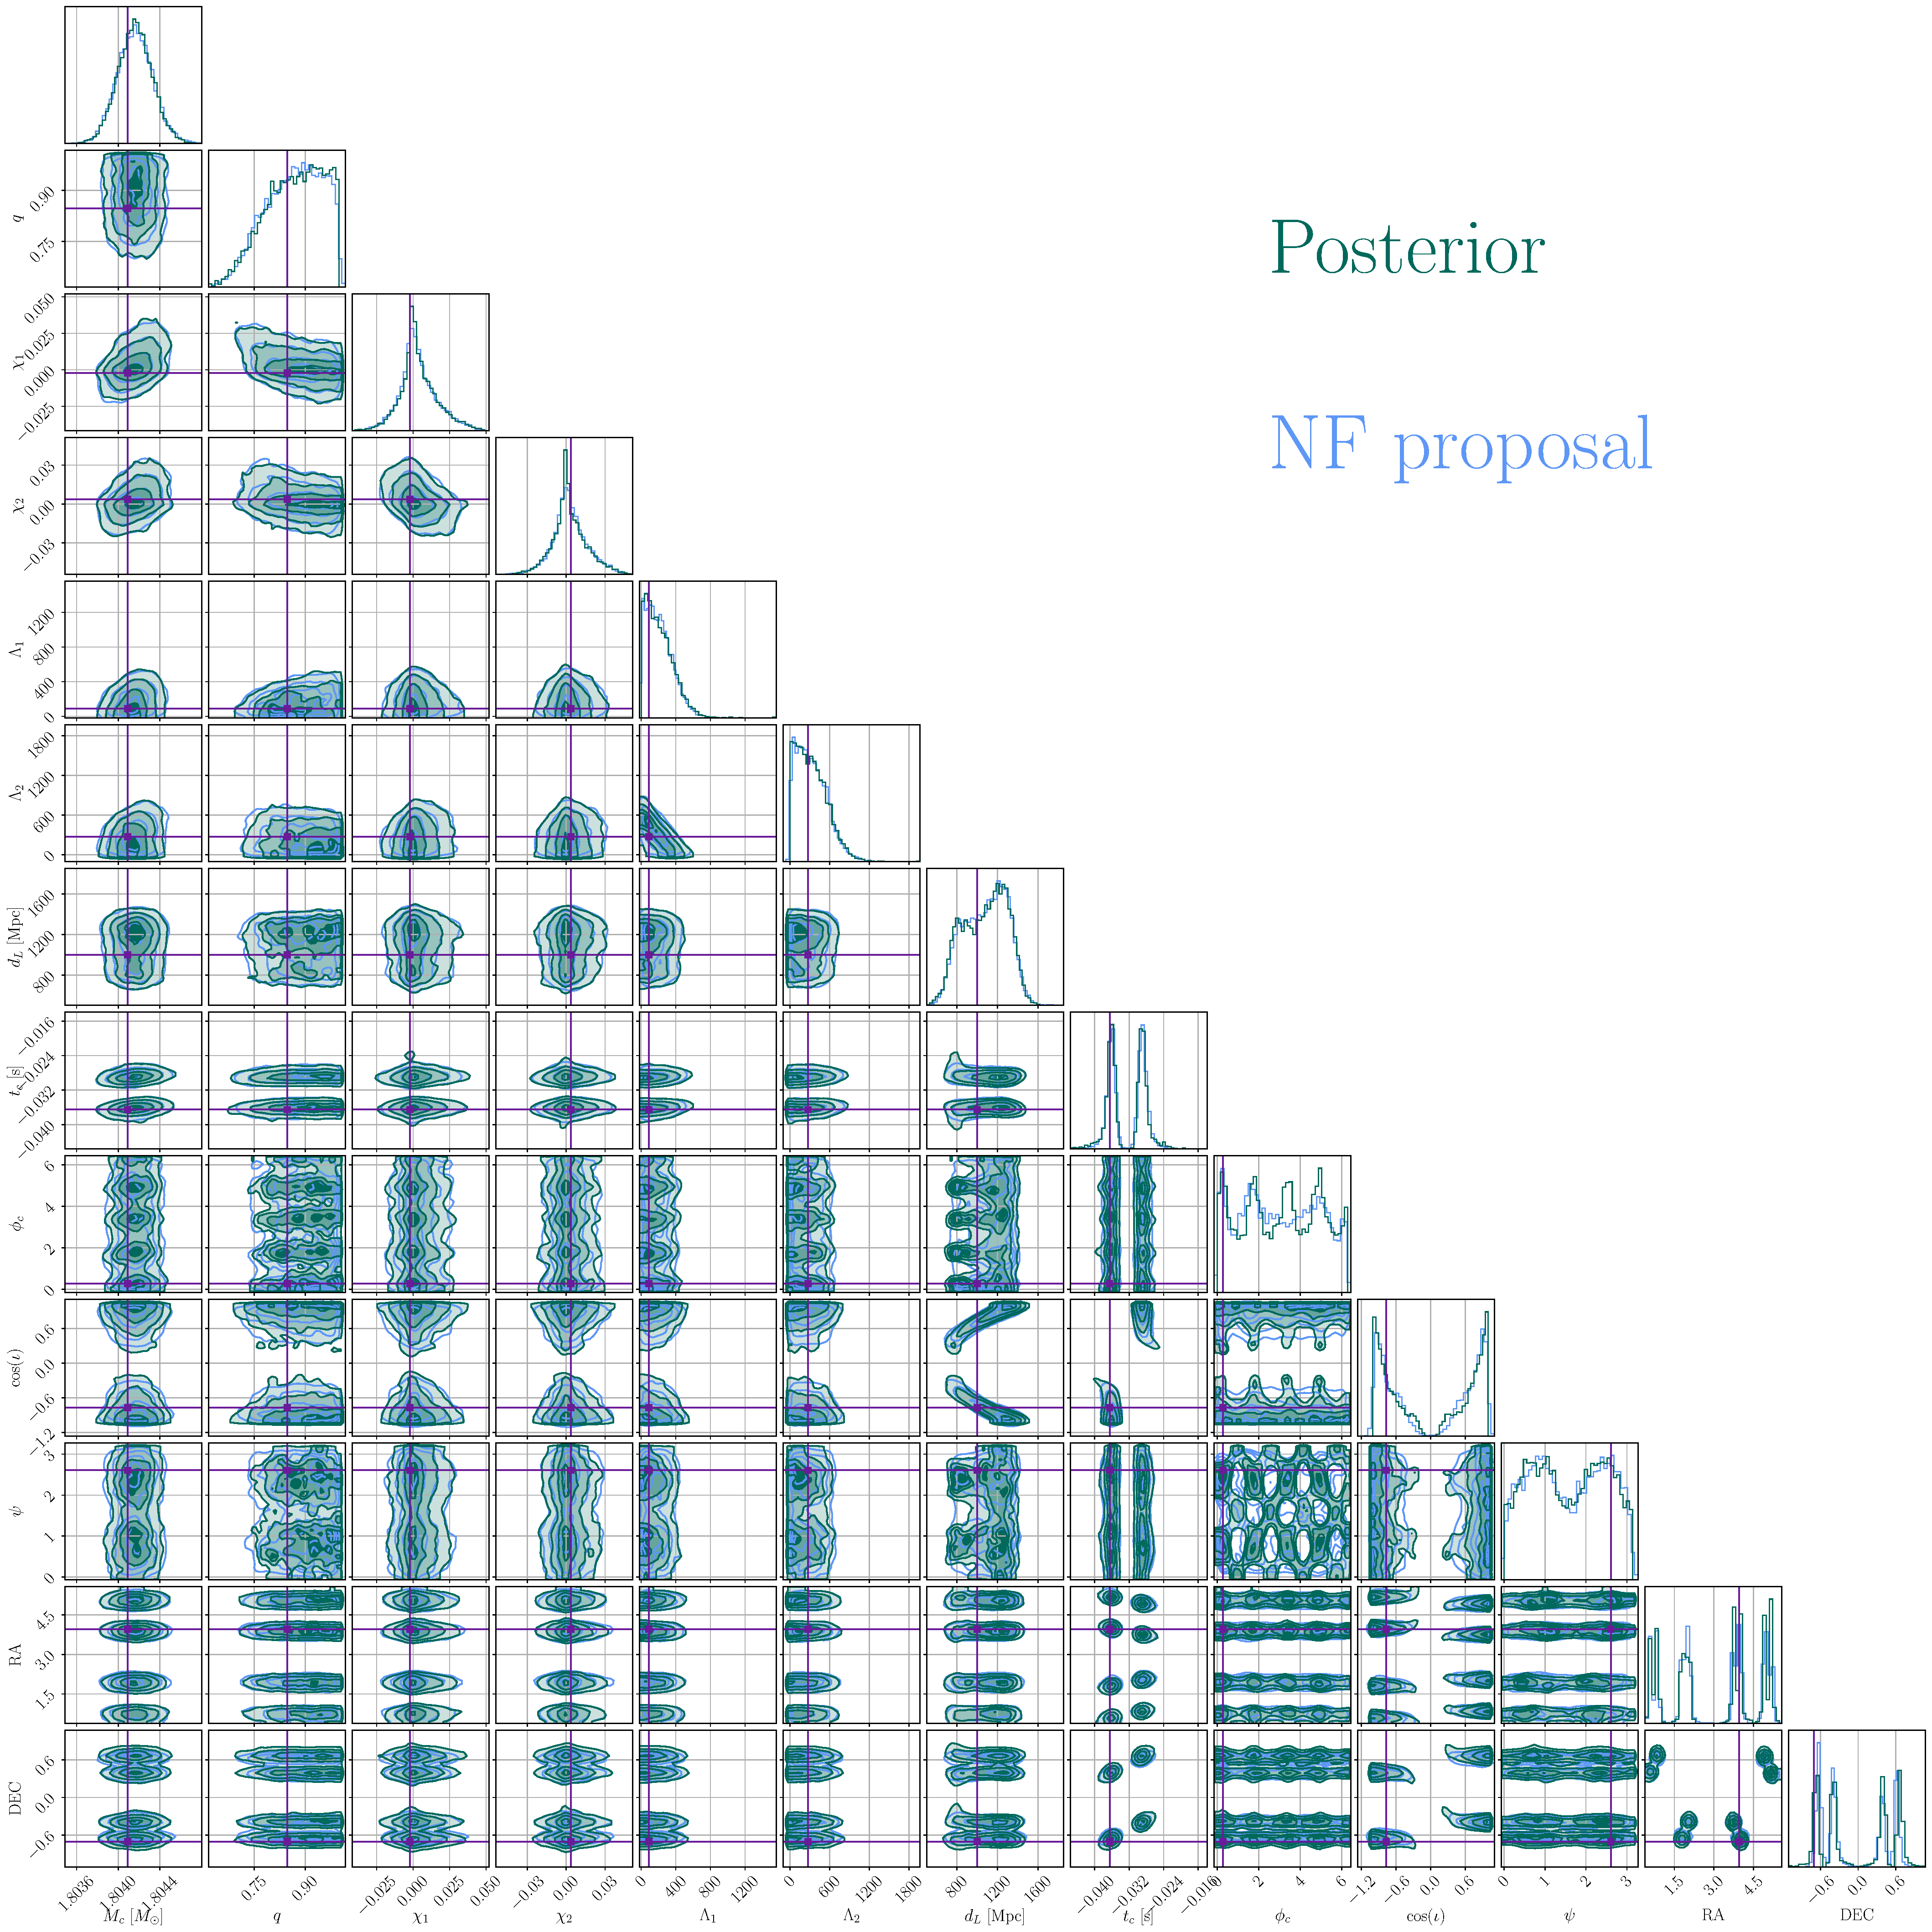
\includegraphics[scale=0.1125]{Figures/corner_plot_big.pdf}
  \end{figure}
\end{frame}

\begin{frame}{Overlapping signals: all parameters signal A}
  \vspace{-3mm}
  \begin{figure}
    \centering
    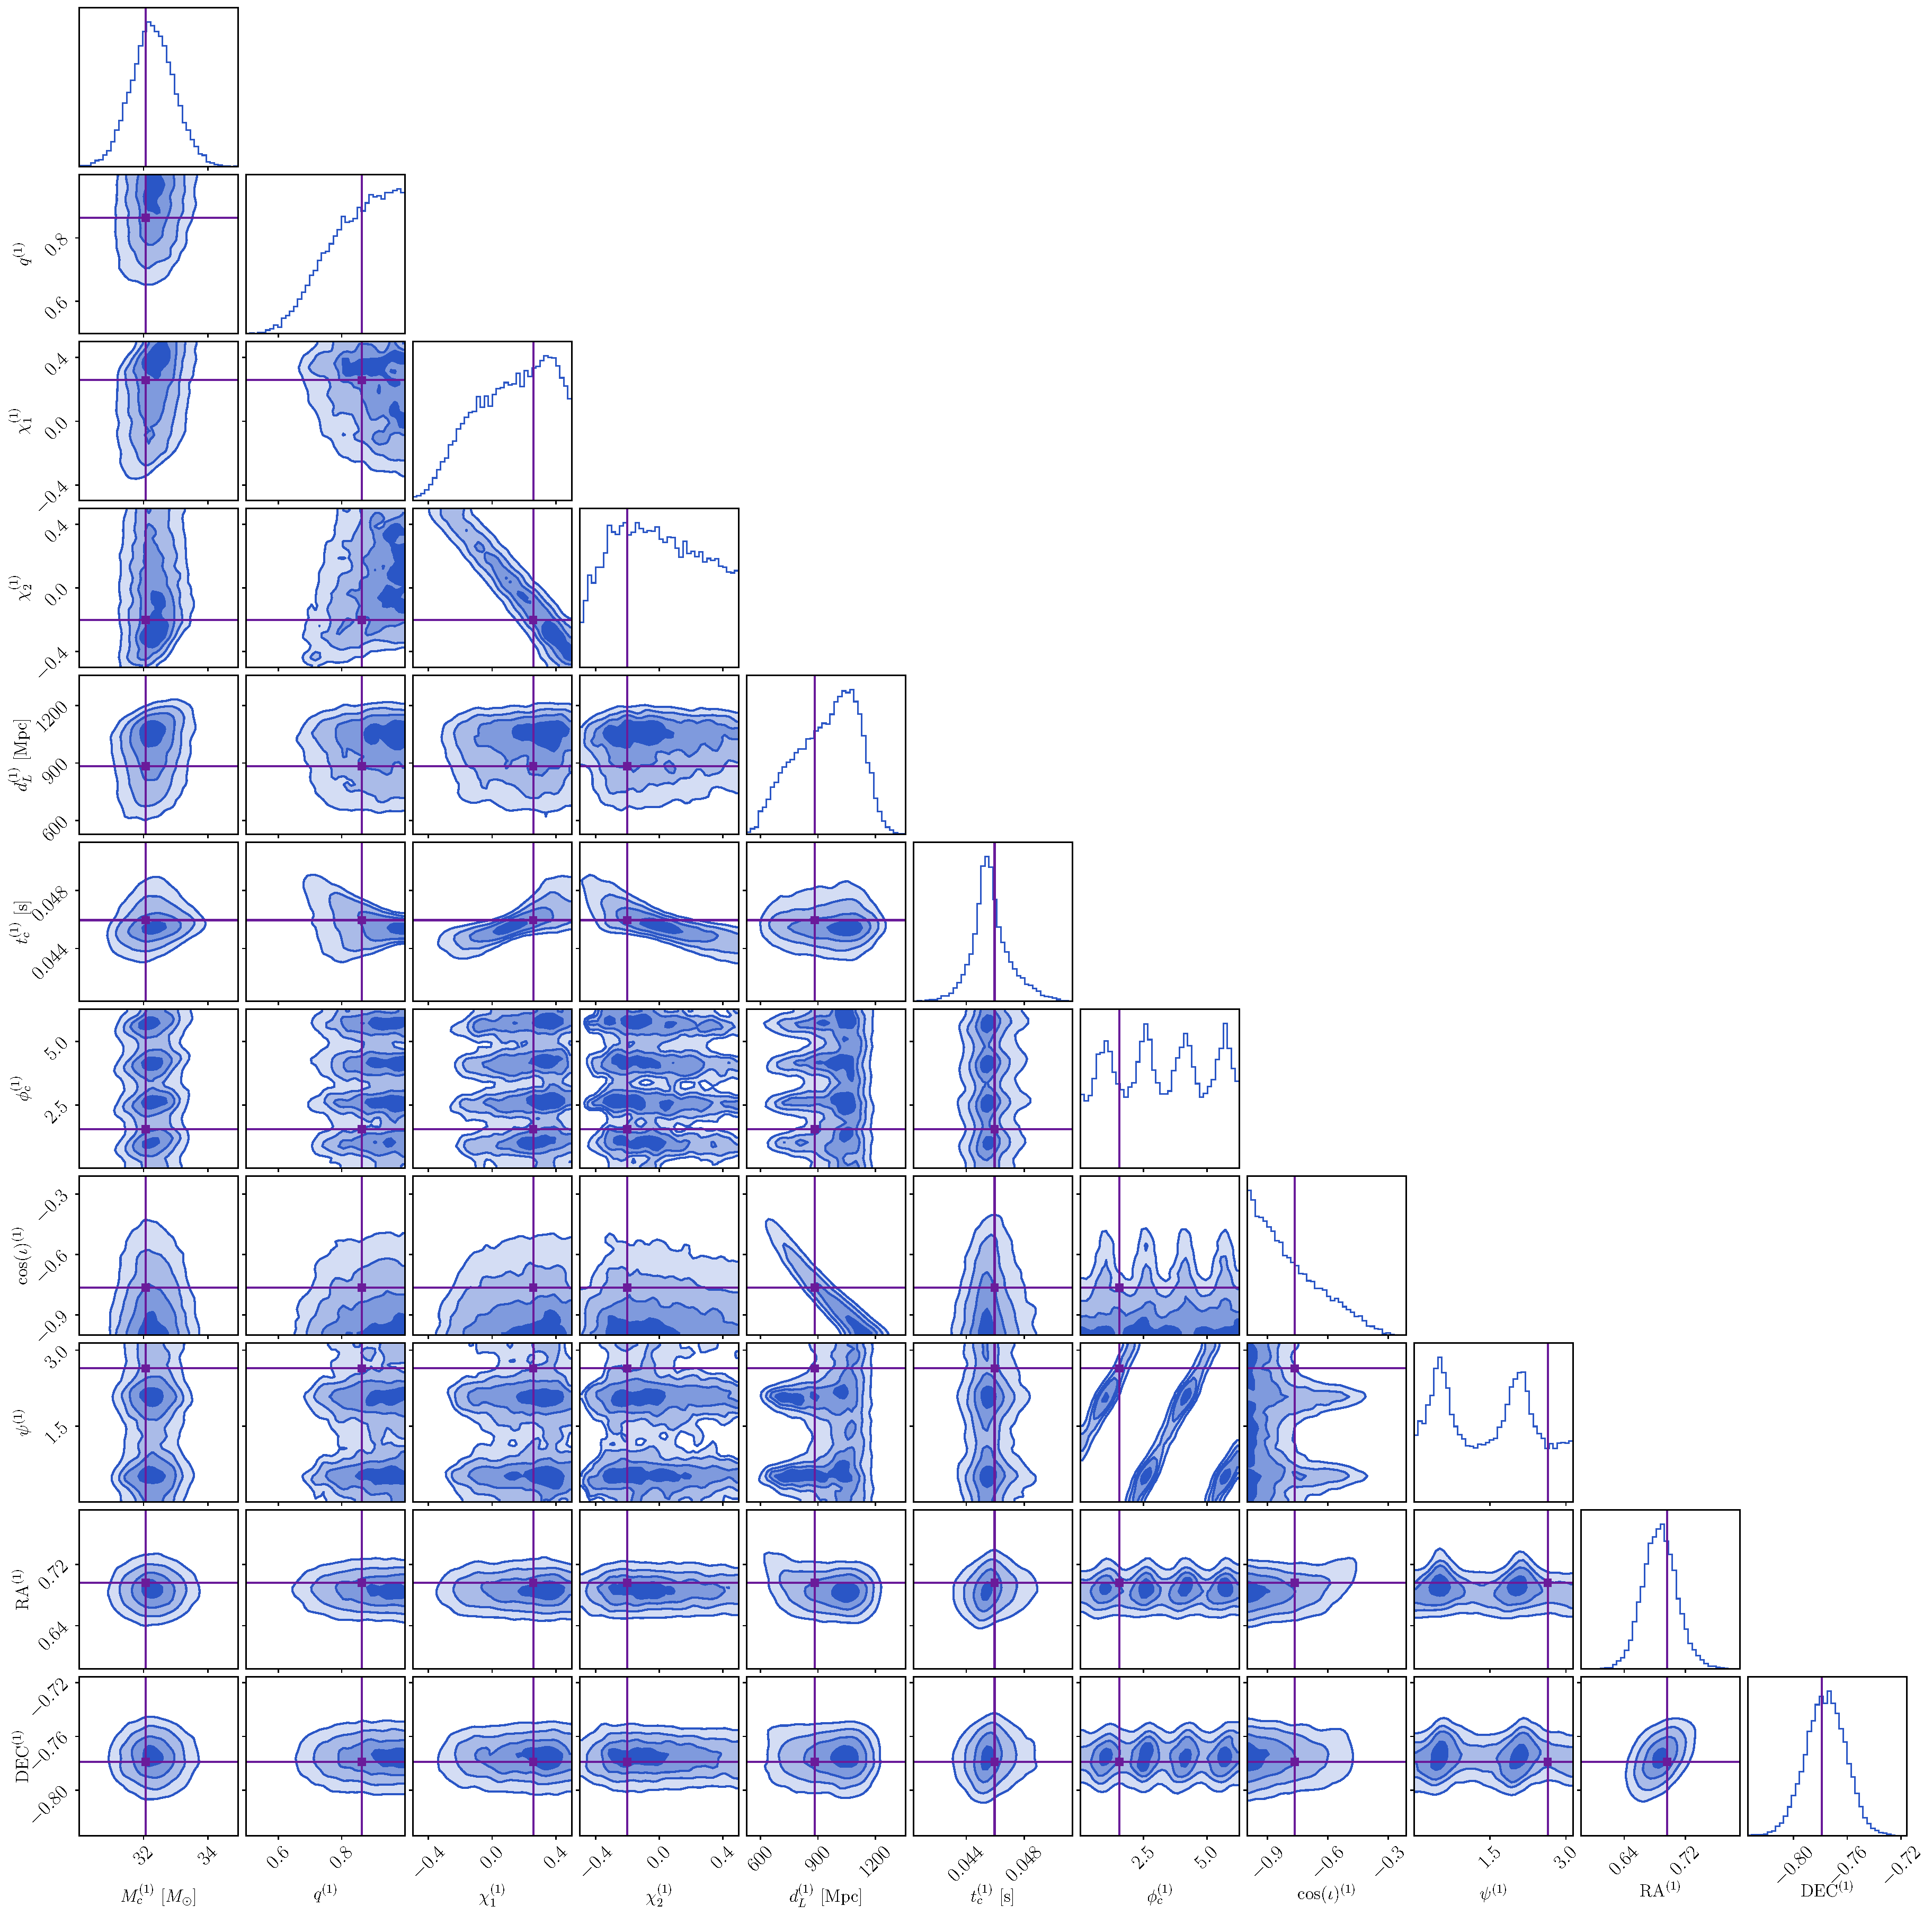
\includegraphics[scale=0.1325]{Figures/OS_injection_139_v2_1_cornerplot_all.pdf}
  \end{figure}
\end{frame}

\begin{frame}{Overlapping signals: all parameters signal B}
  \vspace{-3mm}
  \begin{figure}
    \centering
    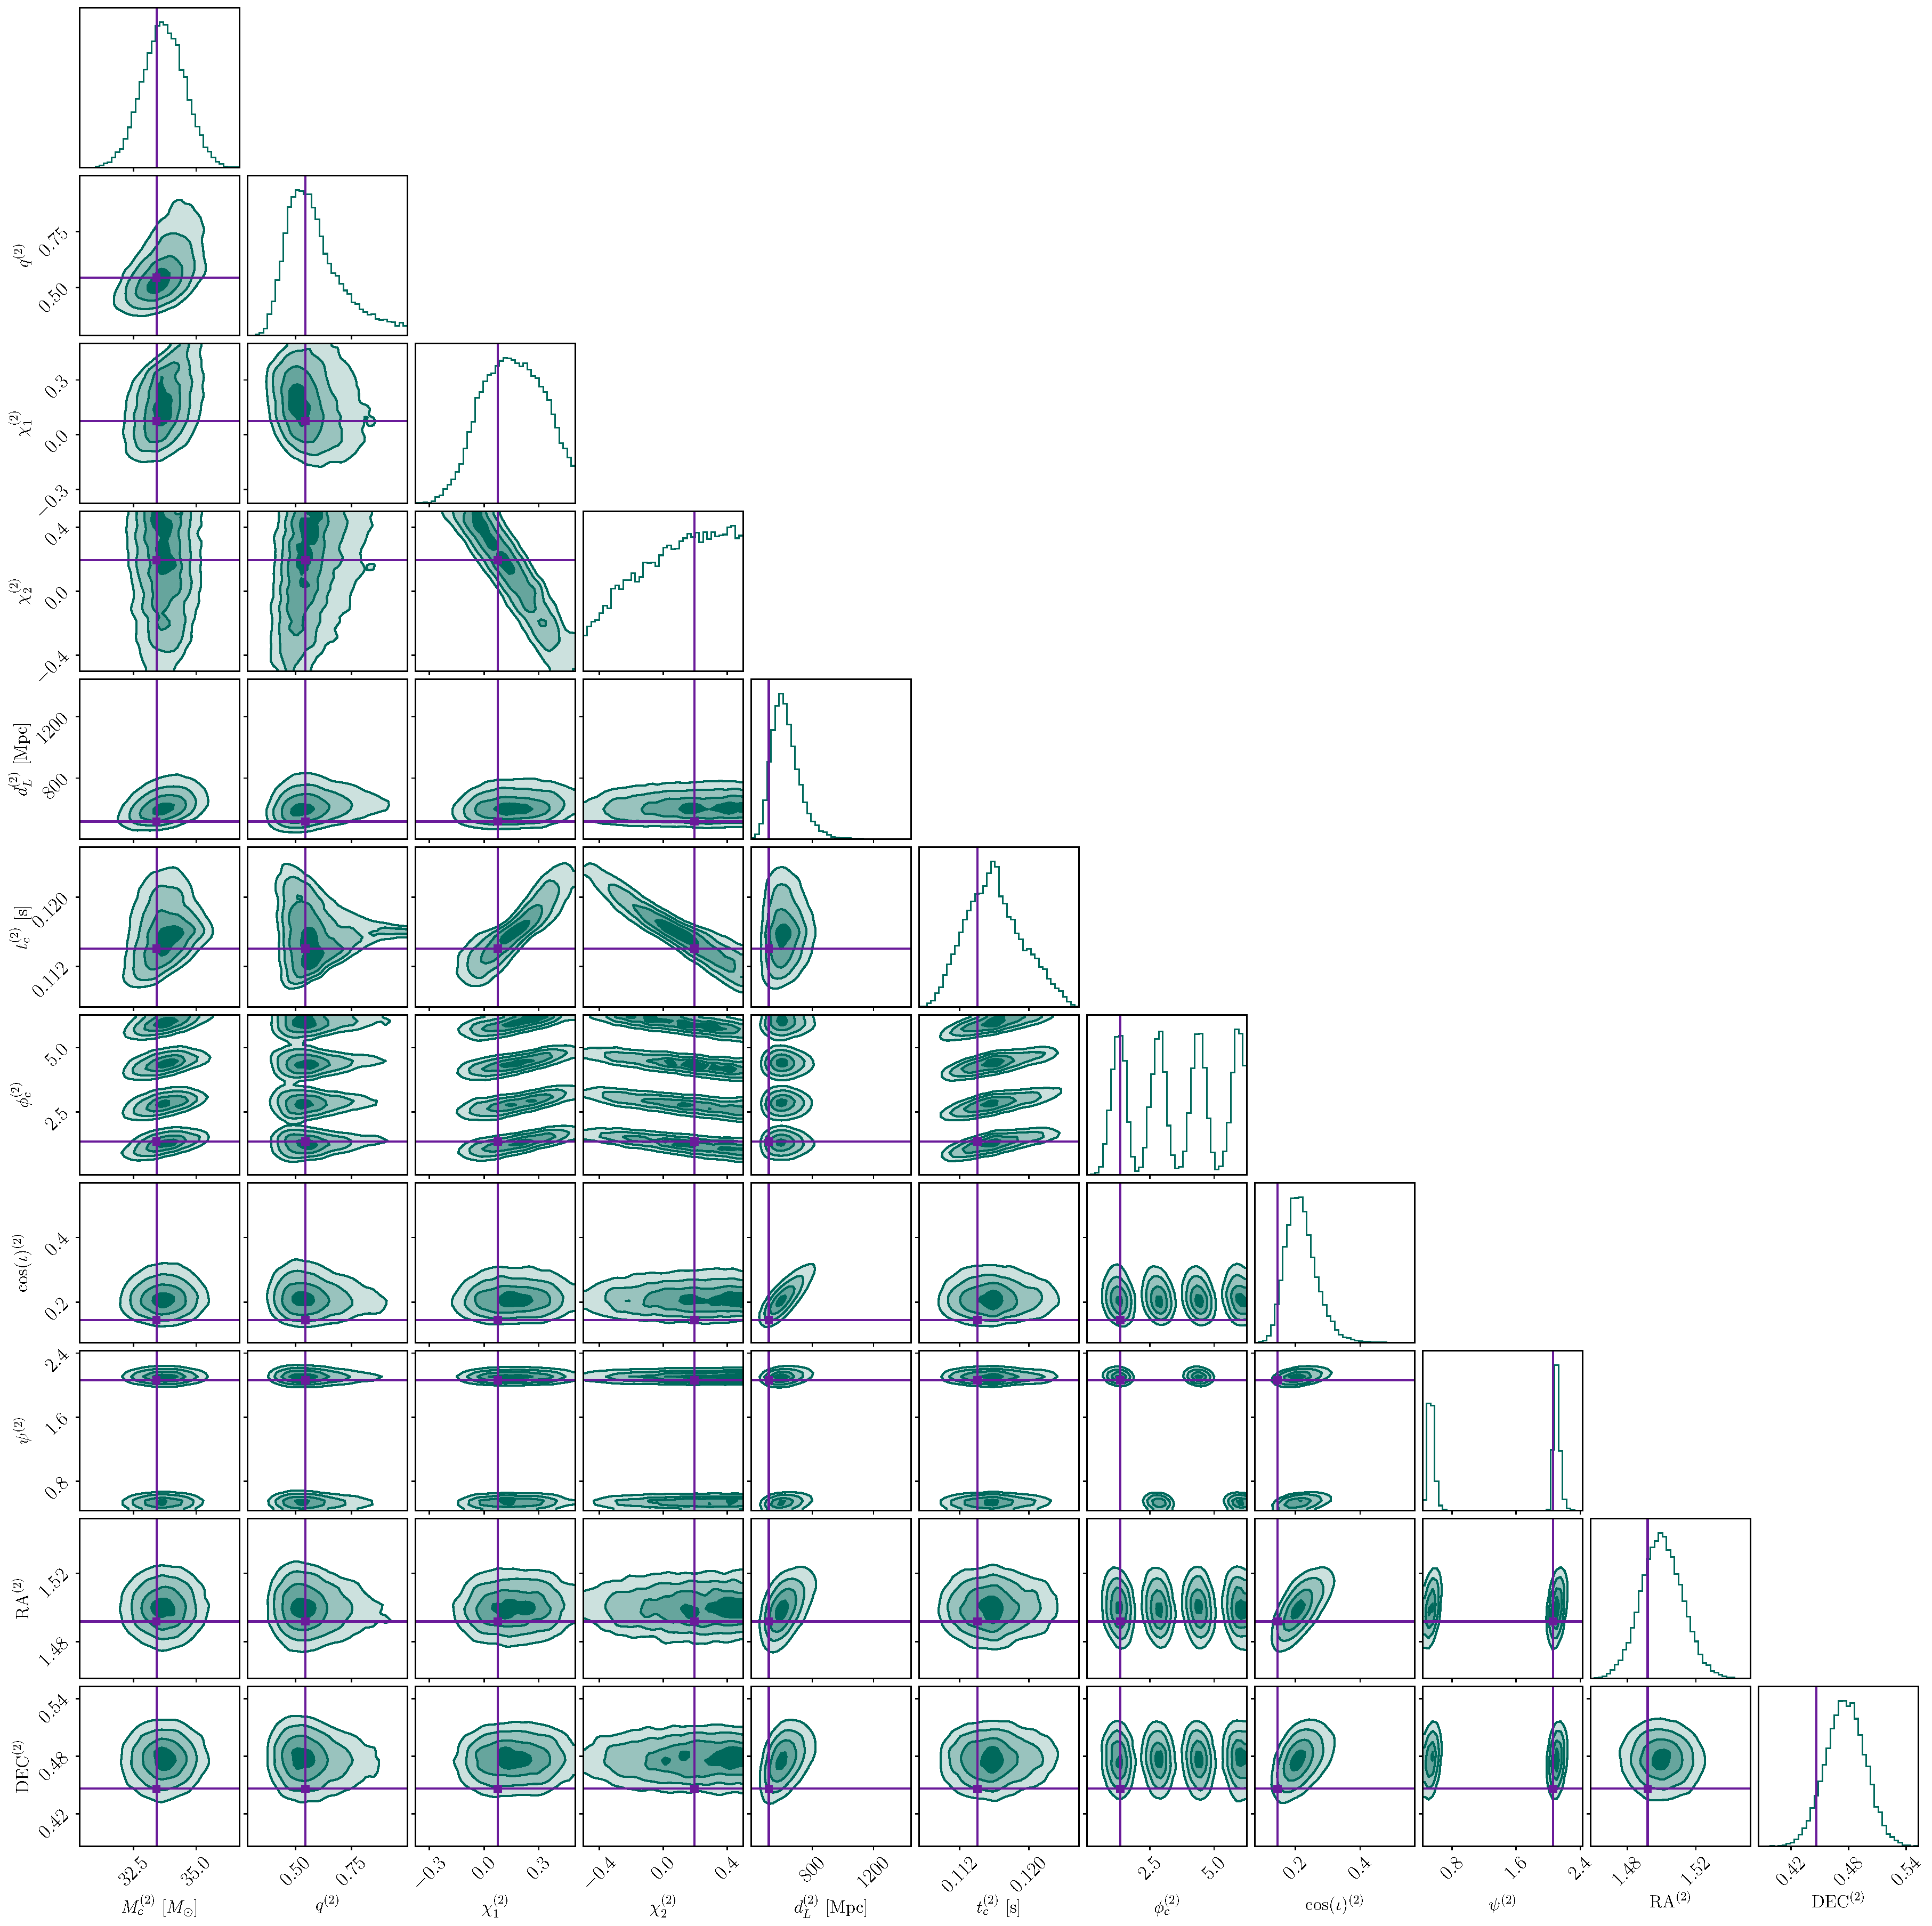
\includegraphics[scale=0.1325]{Figures/OS_injection_139_v2_2_cornerplot_all.pdf}
  \end{figure}
\end{frame}

\begin{frame}{Equation of state O5 projection with 20 BNS: EOS}

  \vspace{-2mm}
  \begin{itemize}
    \item \textbf{\jaxthree{Purple}}: target
    \item \textbf{\red{Red}}: posterior EOS samples (\textbf{black}: maximum log posterior)
  \end{itemize}

  \begin{figure}
    \centering
    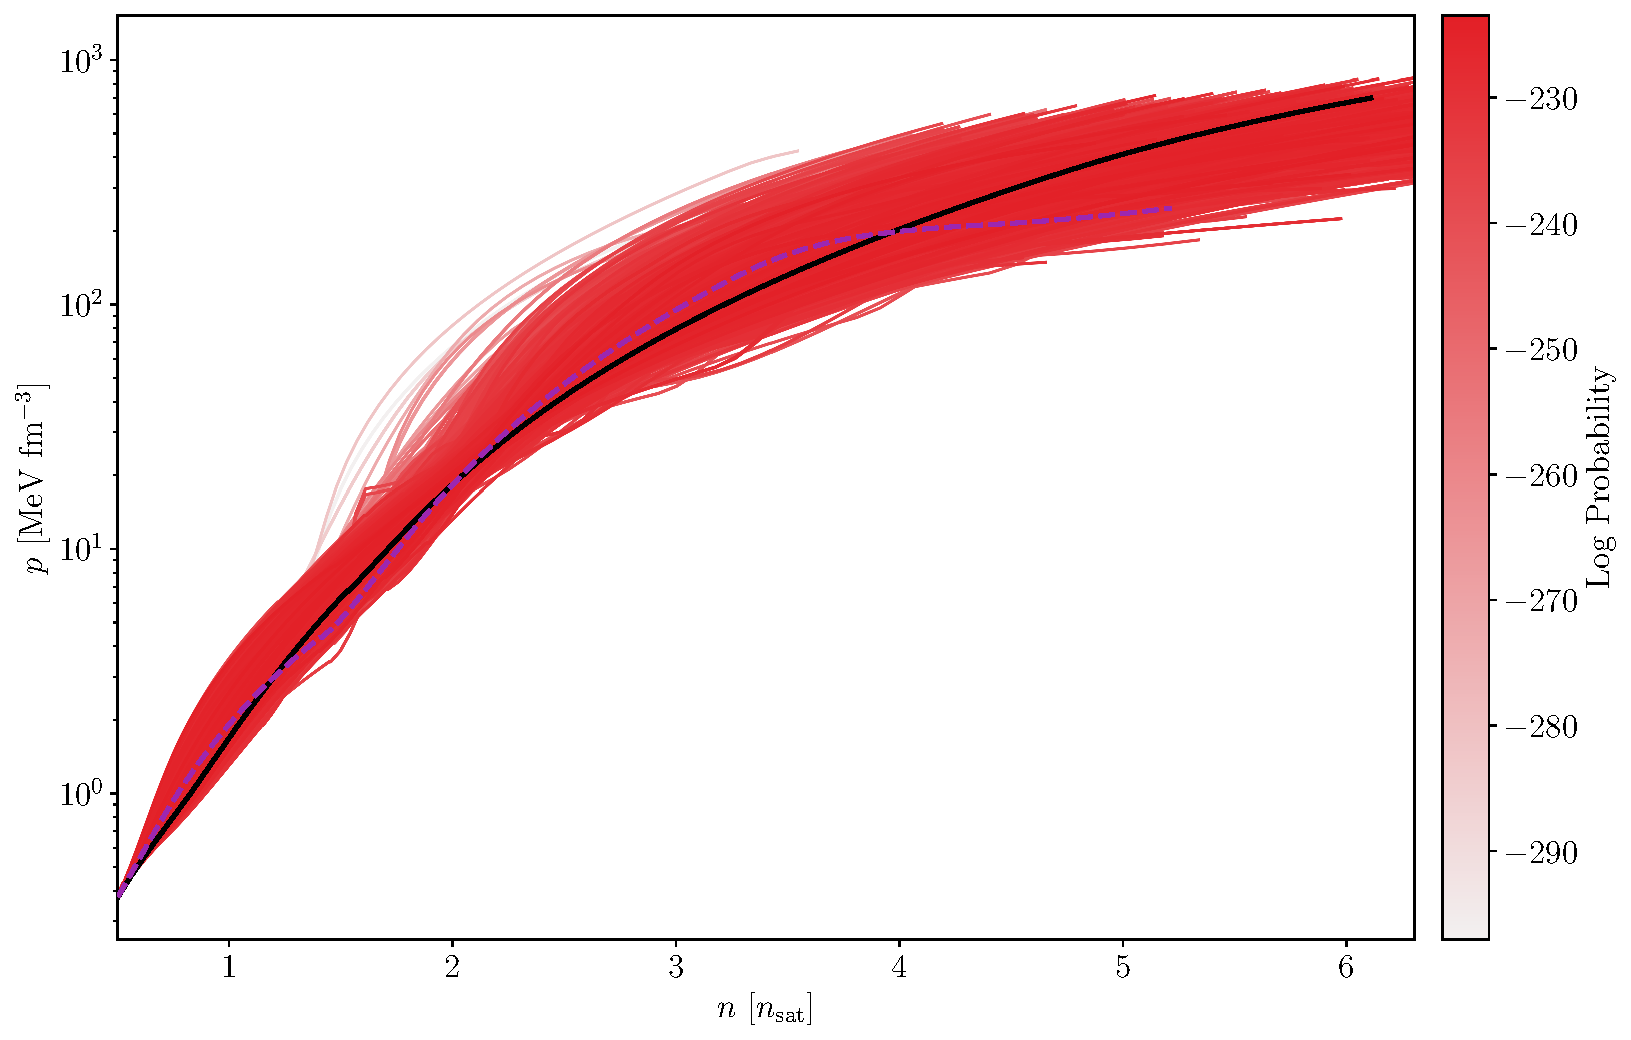
\includegraphics[scale=0.40]{Figures/postprocessing_EOS.pdf}
  \end{figure}
\end{frame}

\begin{frame}{Equation of state O5 projection with 20 BNS: NS}
  \begin{figure}
    \centering
    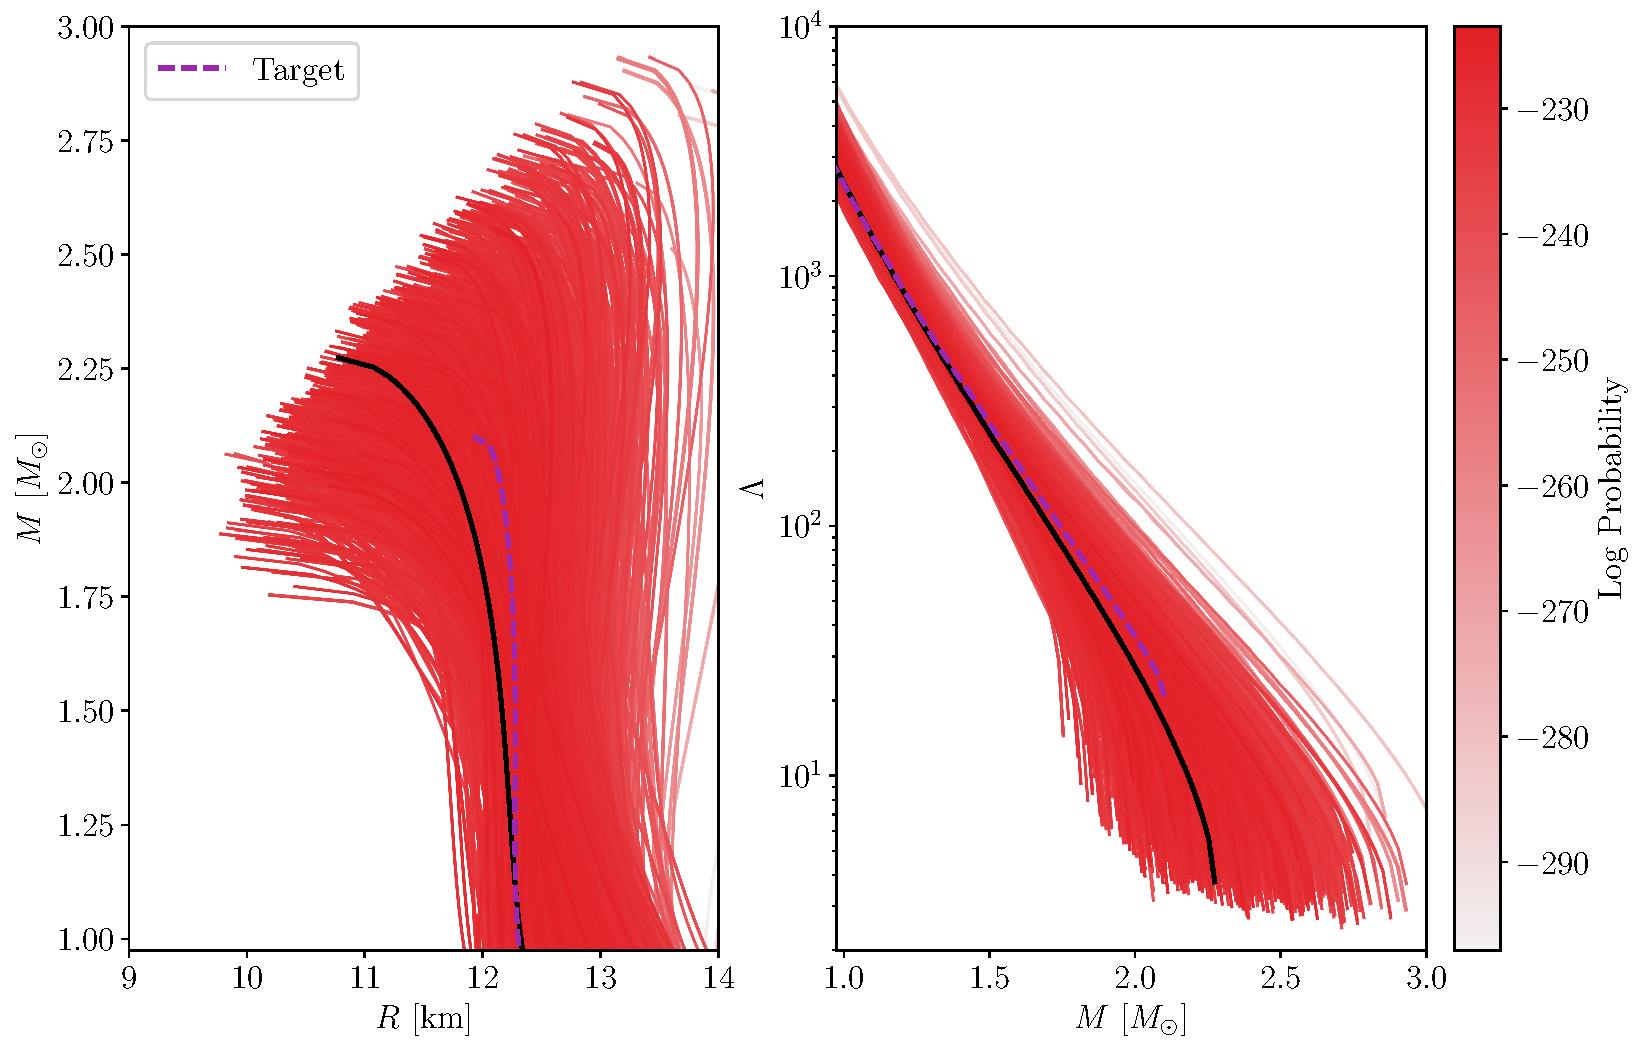
\includegraphics[scale=0.40]{Figures/postprocessing_NS.pdf}
  \end{figure}
\end{frame}


\end{document}